\documentclass[UTF8]{ctexbook}
\usepackage{graphicx}
\usepackage{amsmath}

\title{桥梁大作业报告}
\author{组长:贺琪 \\ 组员:陈煜 \ 刘畅武 \ 杨昊光 \ 朱子霖}

\begin{document}
\maketitle

\tableofcontents

%-------------------------这里是这个项目的整体描述---------------------------------
%----------------------------------------------------------------------------------
\newpage
\section{总述}
\subsection{项目描述}
桥模型由桥墩(pier),桥面(floor),支撑梁(support beam),河堤(river bank)和钢缆(cables)五部分组成,其中桥墩和河堤用实体单元建模,桥面用板单元建模,支撑梁用梁单元建模,钢缆用杆单元建模,如图1 所示。\\
\begin{center}
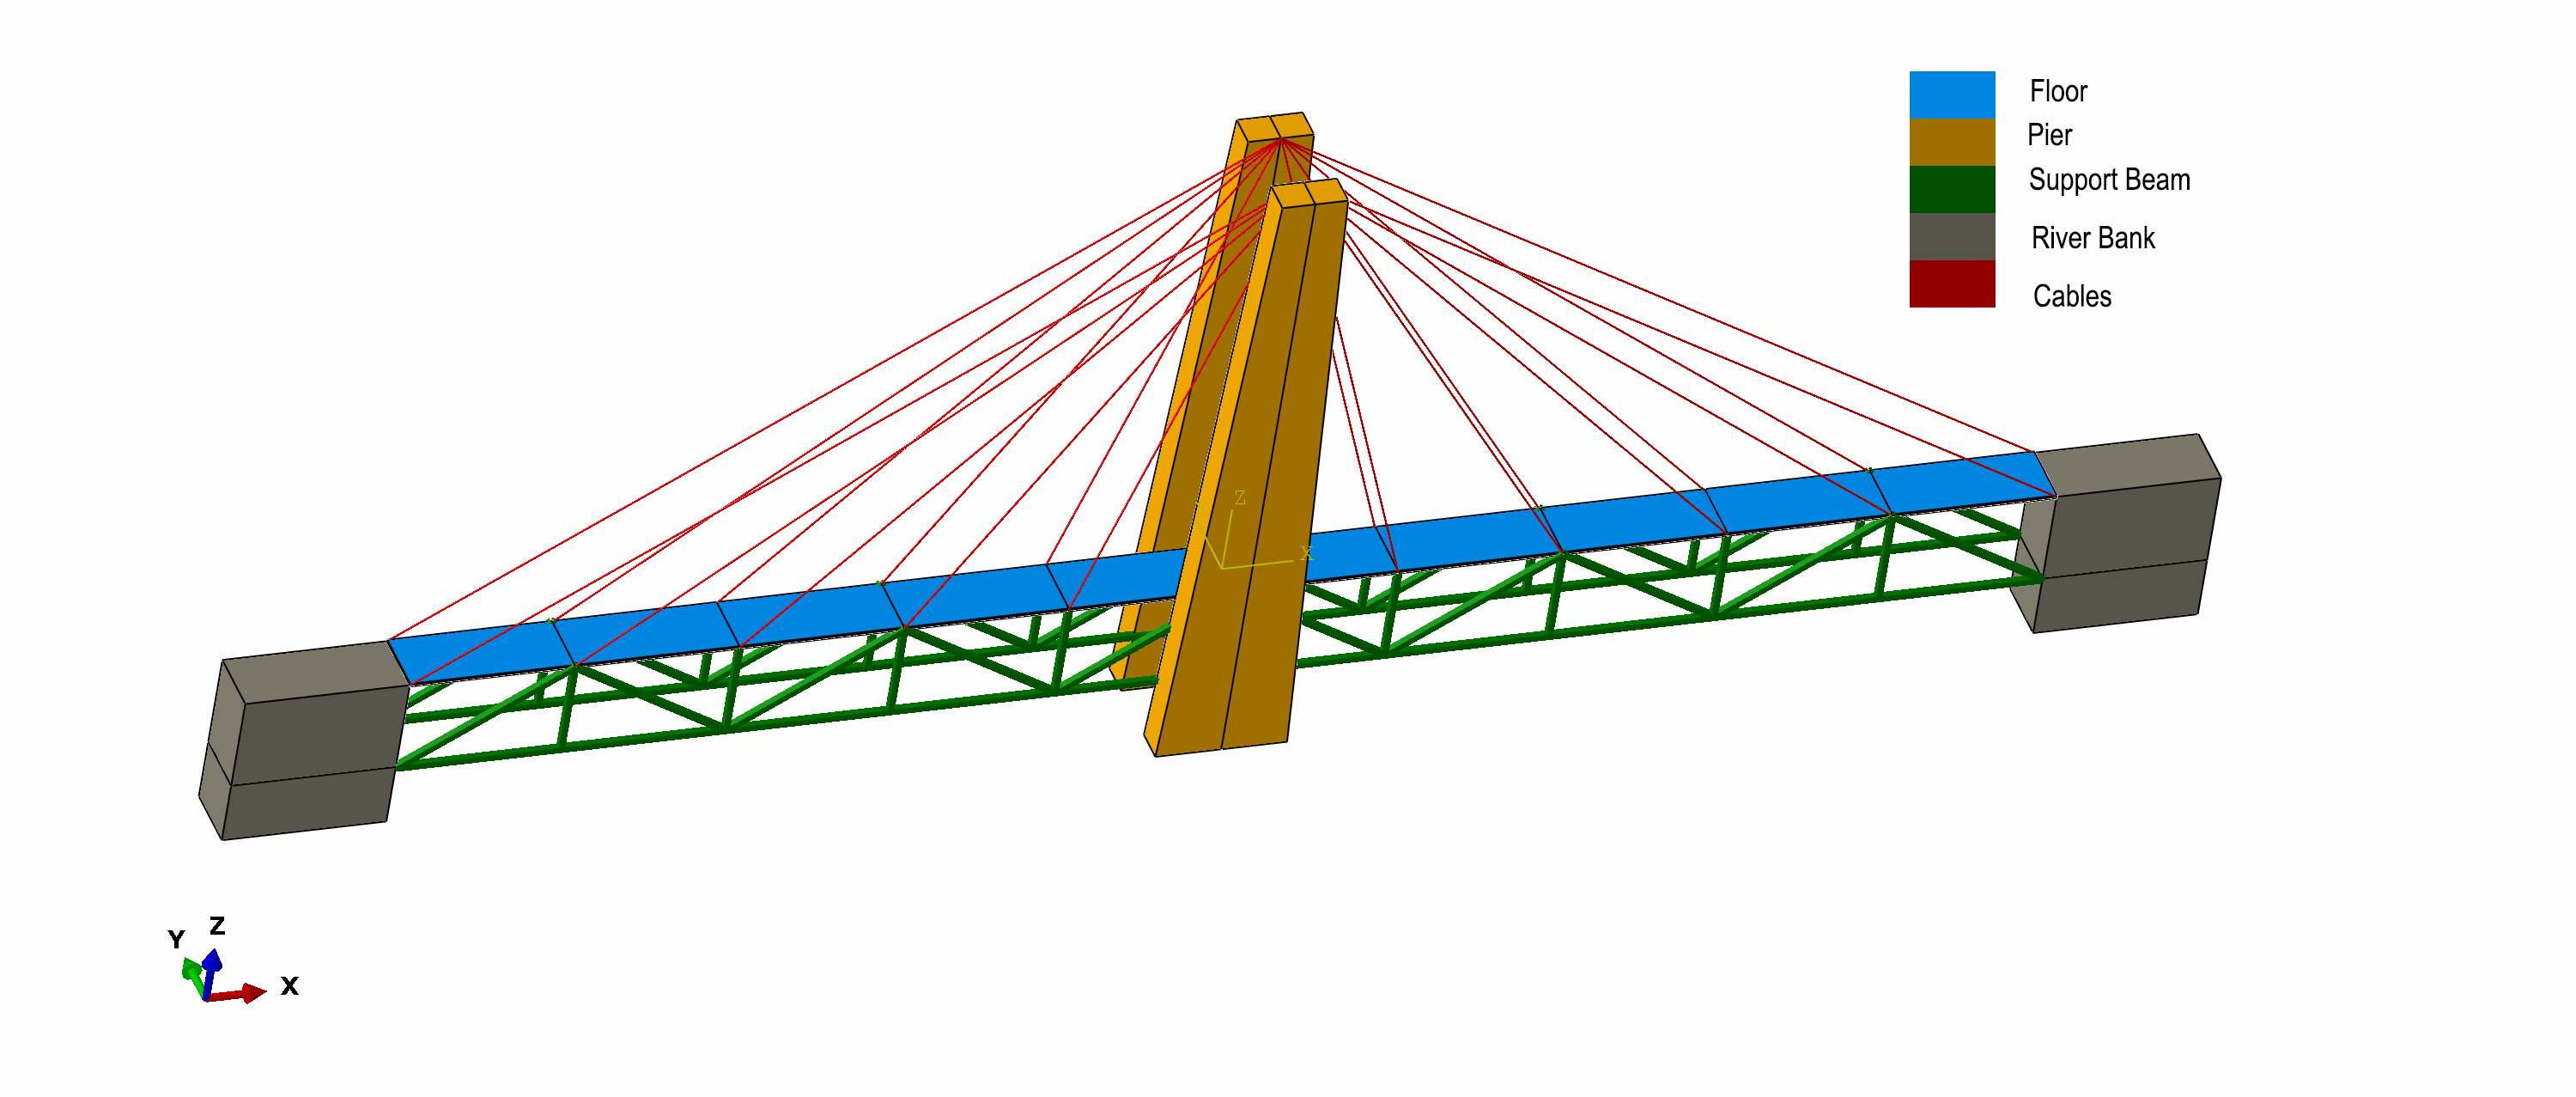
\includegraphics[width=0.6\textwidth]{01.png} % Include the image placeholder.png
\end{center}

\textbf{桥墩}:

桥墩在XZ方向为左右对称梯形,如图2所示,梯形高200,上底为20,下底40,在y方向上厚度为10。桥面位于距桥墩底50处。两个桥墩顶面内侧中点为所有钢缆的与桥墩的连接点。(参照图1)

采用实体单元建模

\begin{center}
\begin{tabular}{ll}
材料&:Concrete\\
弹性模量&:25e9\\
泊松比&:0.3\\
密度&:2320\\
\end{tabular}
\end{center}

\begin{center}
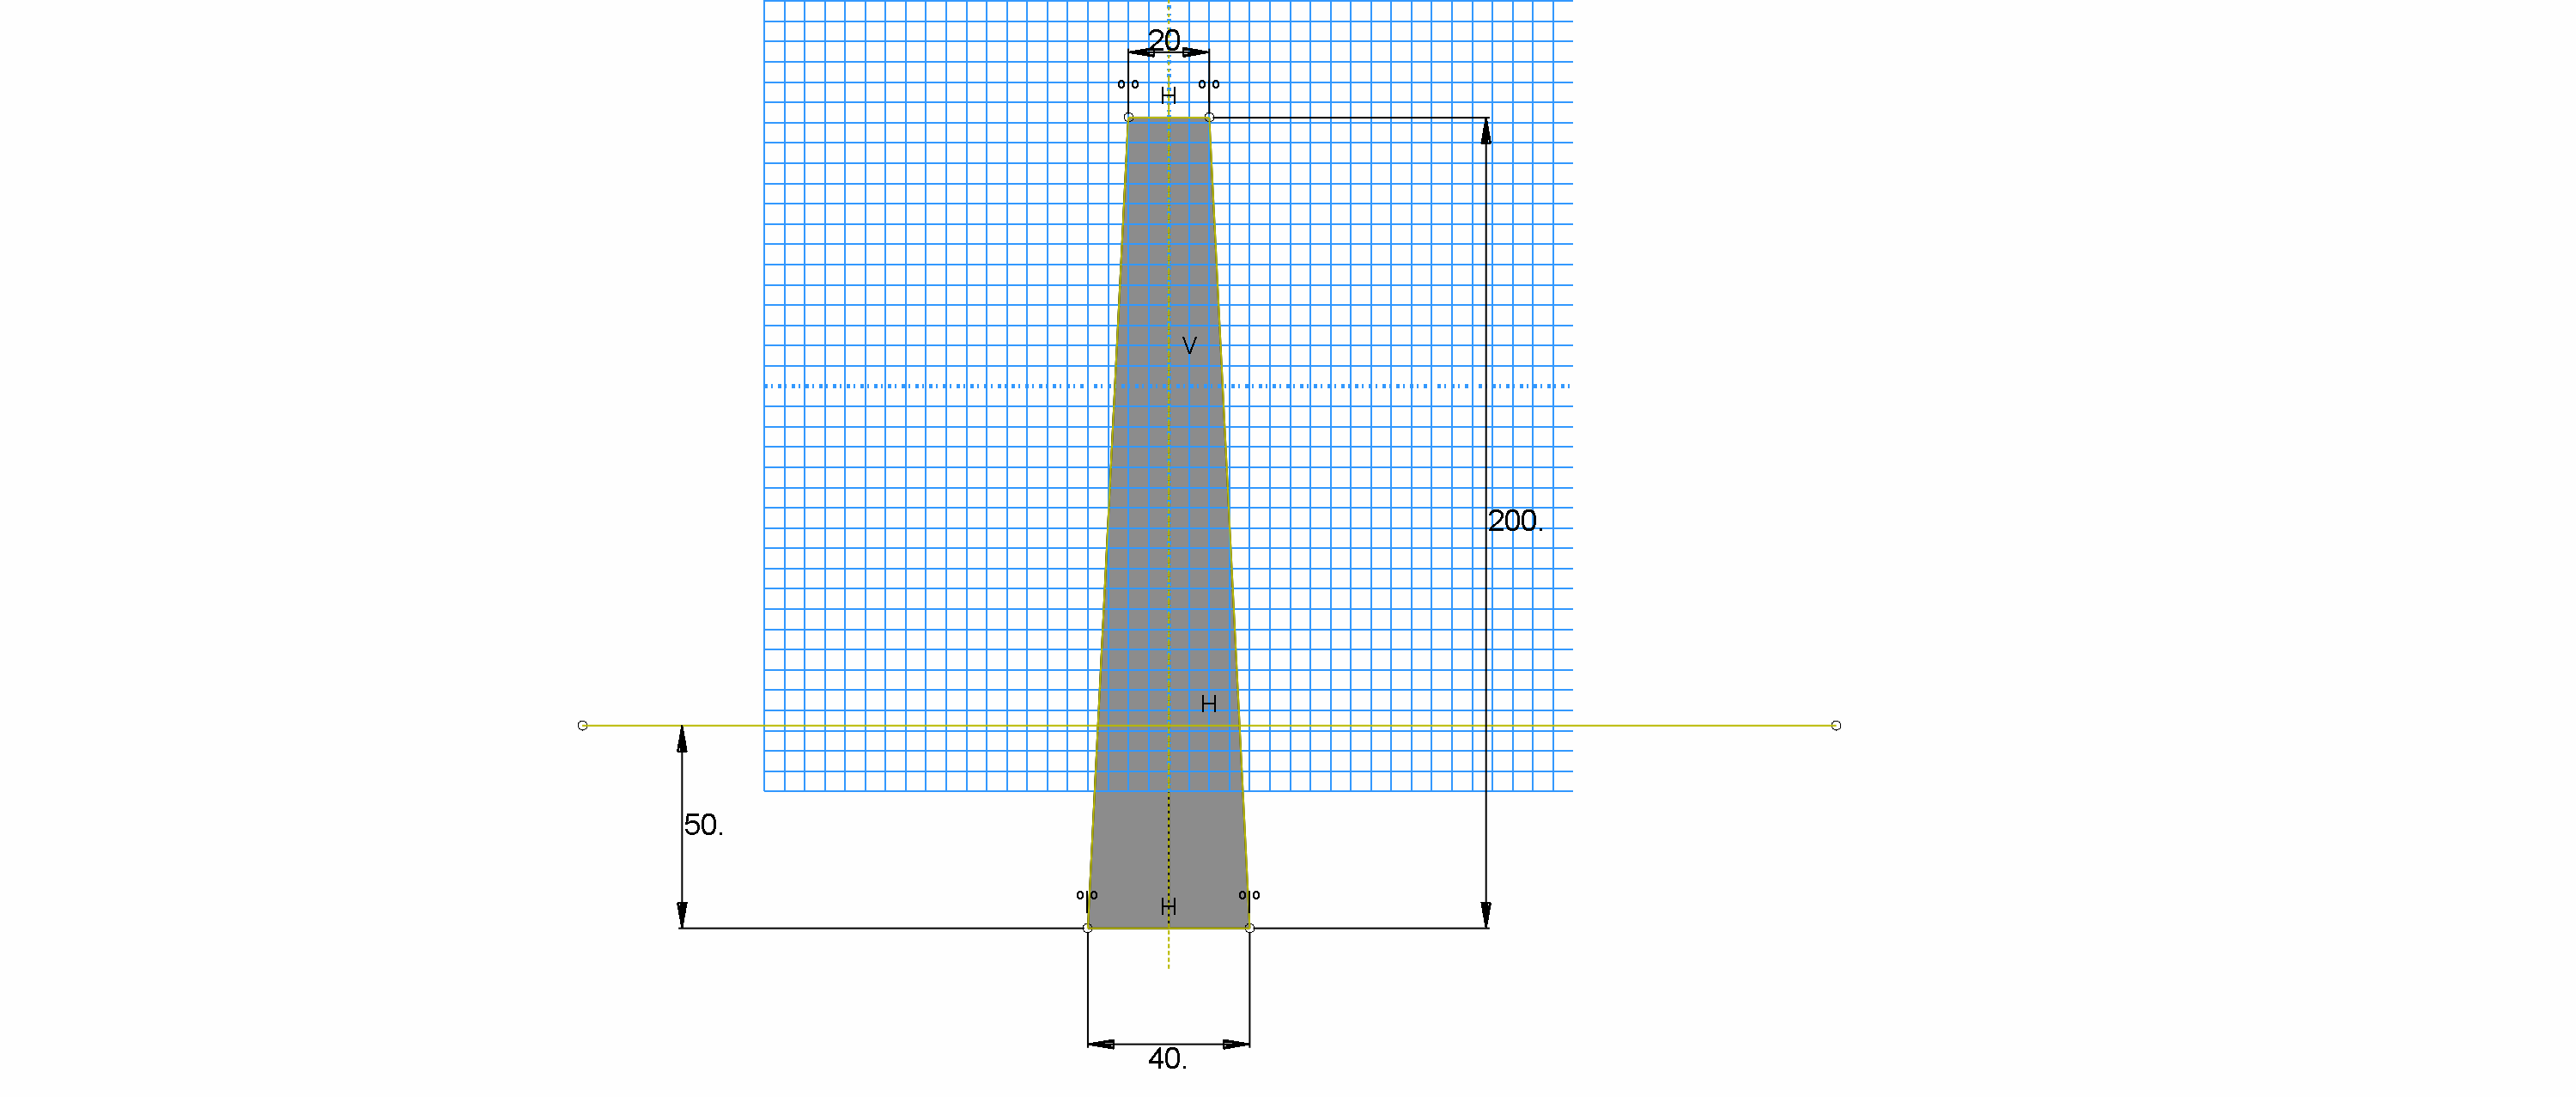
\includegraphics[width=0.6\textwidth]{02.png}
\end{center}

\textbf{桥面}:

桥面位于z=0的平面内,如图3所示,为长方形,长为500,宽为20,厚度为1。在桥面上下边对称地布置钢缆连接点,每个钢缆连接点相距50,共计2×2×5=20个钢缆连接点。每根钢缆另一端连接桥墩顶面内侧中点。(参照图1)

采用板单元建模

\begin{center}
\begin{tabular}{ll}
材料&:Concrete\\
弹性模量&:25e9\\
泊松比&:0.3\\
密度&:2320\\
\end{tabular}
\end{center}
\begin{center}
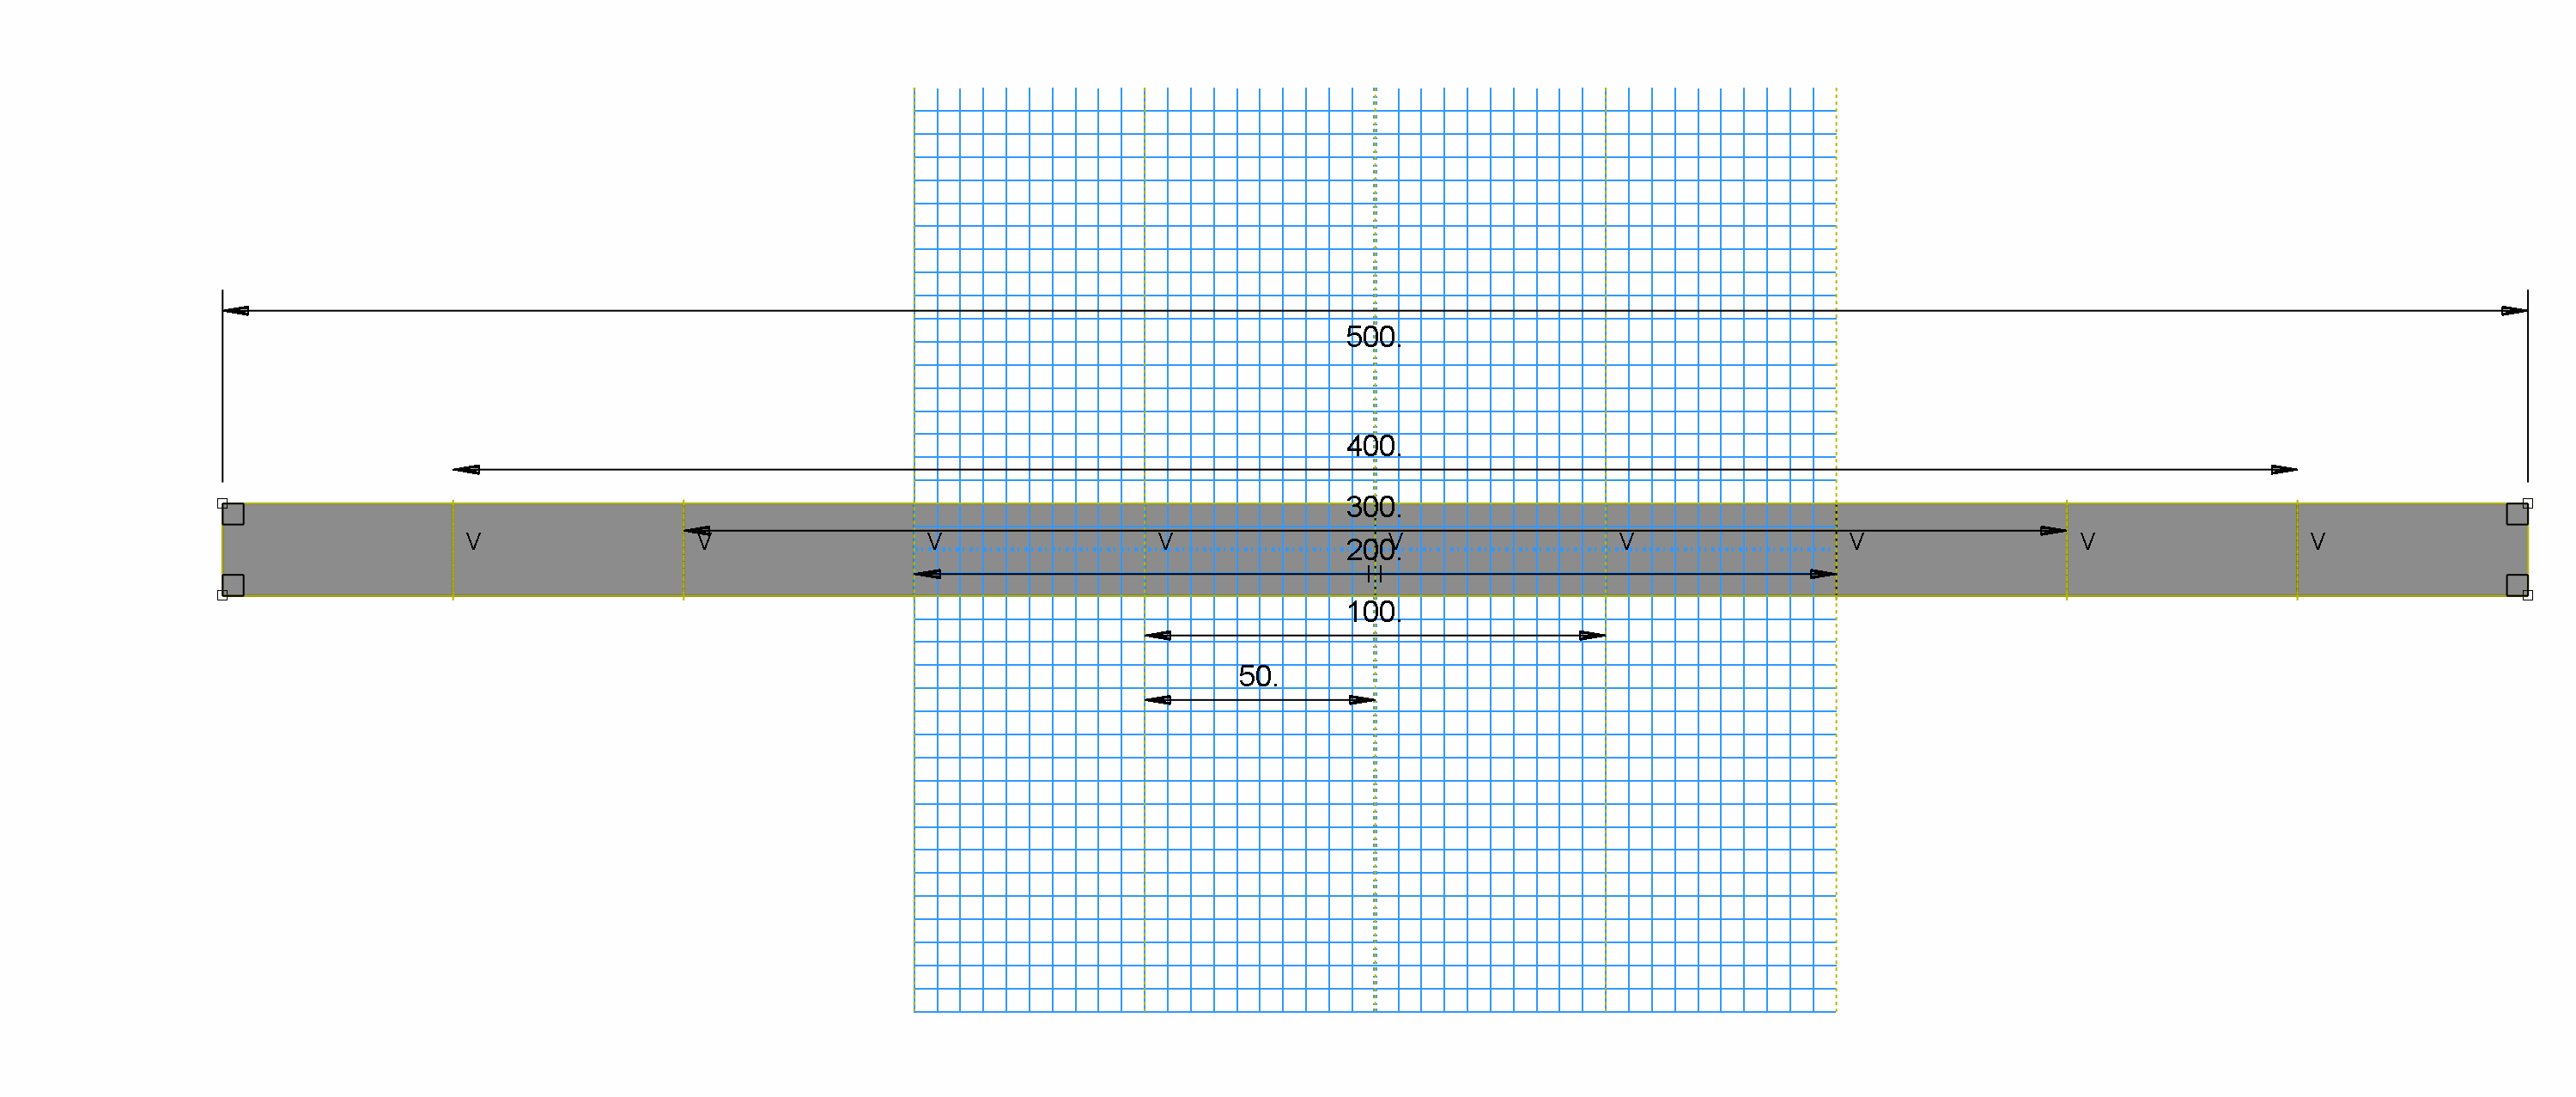
\includegraphics[width=0.6\textwidth]{03.png}
\end{center}

\textbf{河堤}:

河堤为50×50×20的立方体,如图1所示,变长为20的一边与桥面相铰接,另外在距离底面20处与支撑梁相铰接。(铰接指对应结点平动自由度相同,转动自由度自由)

采用实体单元建模。

\begin{center}
\begin{tabular}{ll}
材料&:Granite\\
弹性模量&:60e9\\
泊松比&:0.27\\
密度&:2770\\
\end{tabular}
\end{center}

\textbf{支撑梁}:

支撑梁共有两组,分别位于桥面两侧下方,其结构左右对称,如图4所示。支撑梁上部每个结点与桥面相铰接,两组共计2×9=18个结点。两端结点与河堤相铰接,共计2×2=4个结点。

采用梁单元建模,梁截面为正方形筒,边长为2,厚度为0.1。

\begin{center}
\begin{tabular}{ll}
材料&:Aluminum\\
弹性模量&:70e9\\
泊松比&:0.346\\
密度&:2710\\
\end{tabular}
\end{center}
\begin{center}
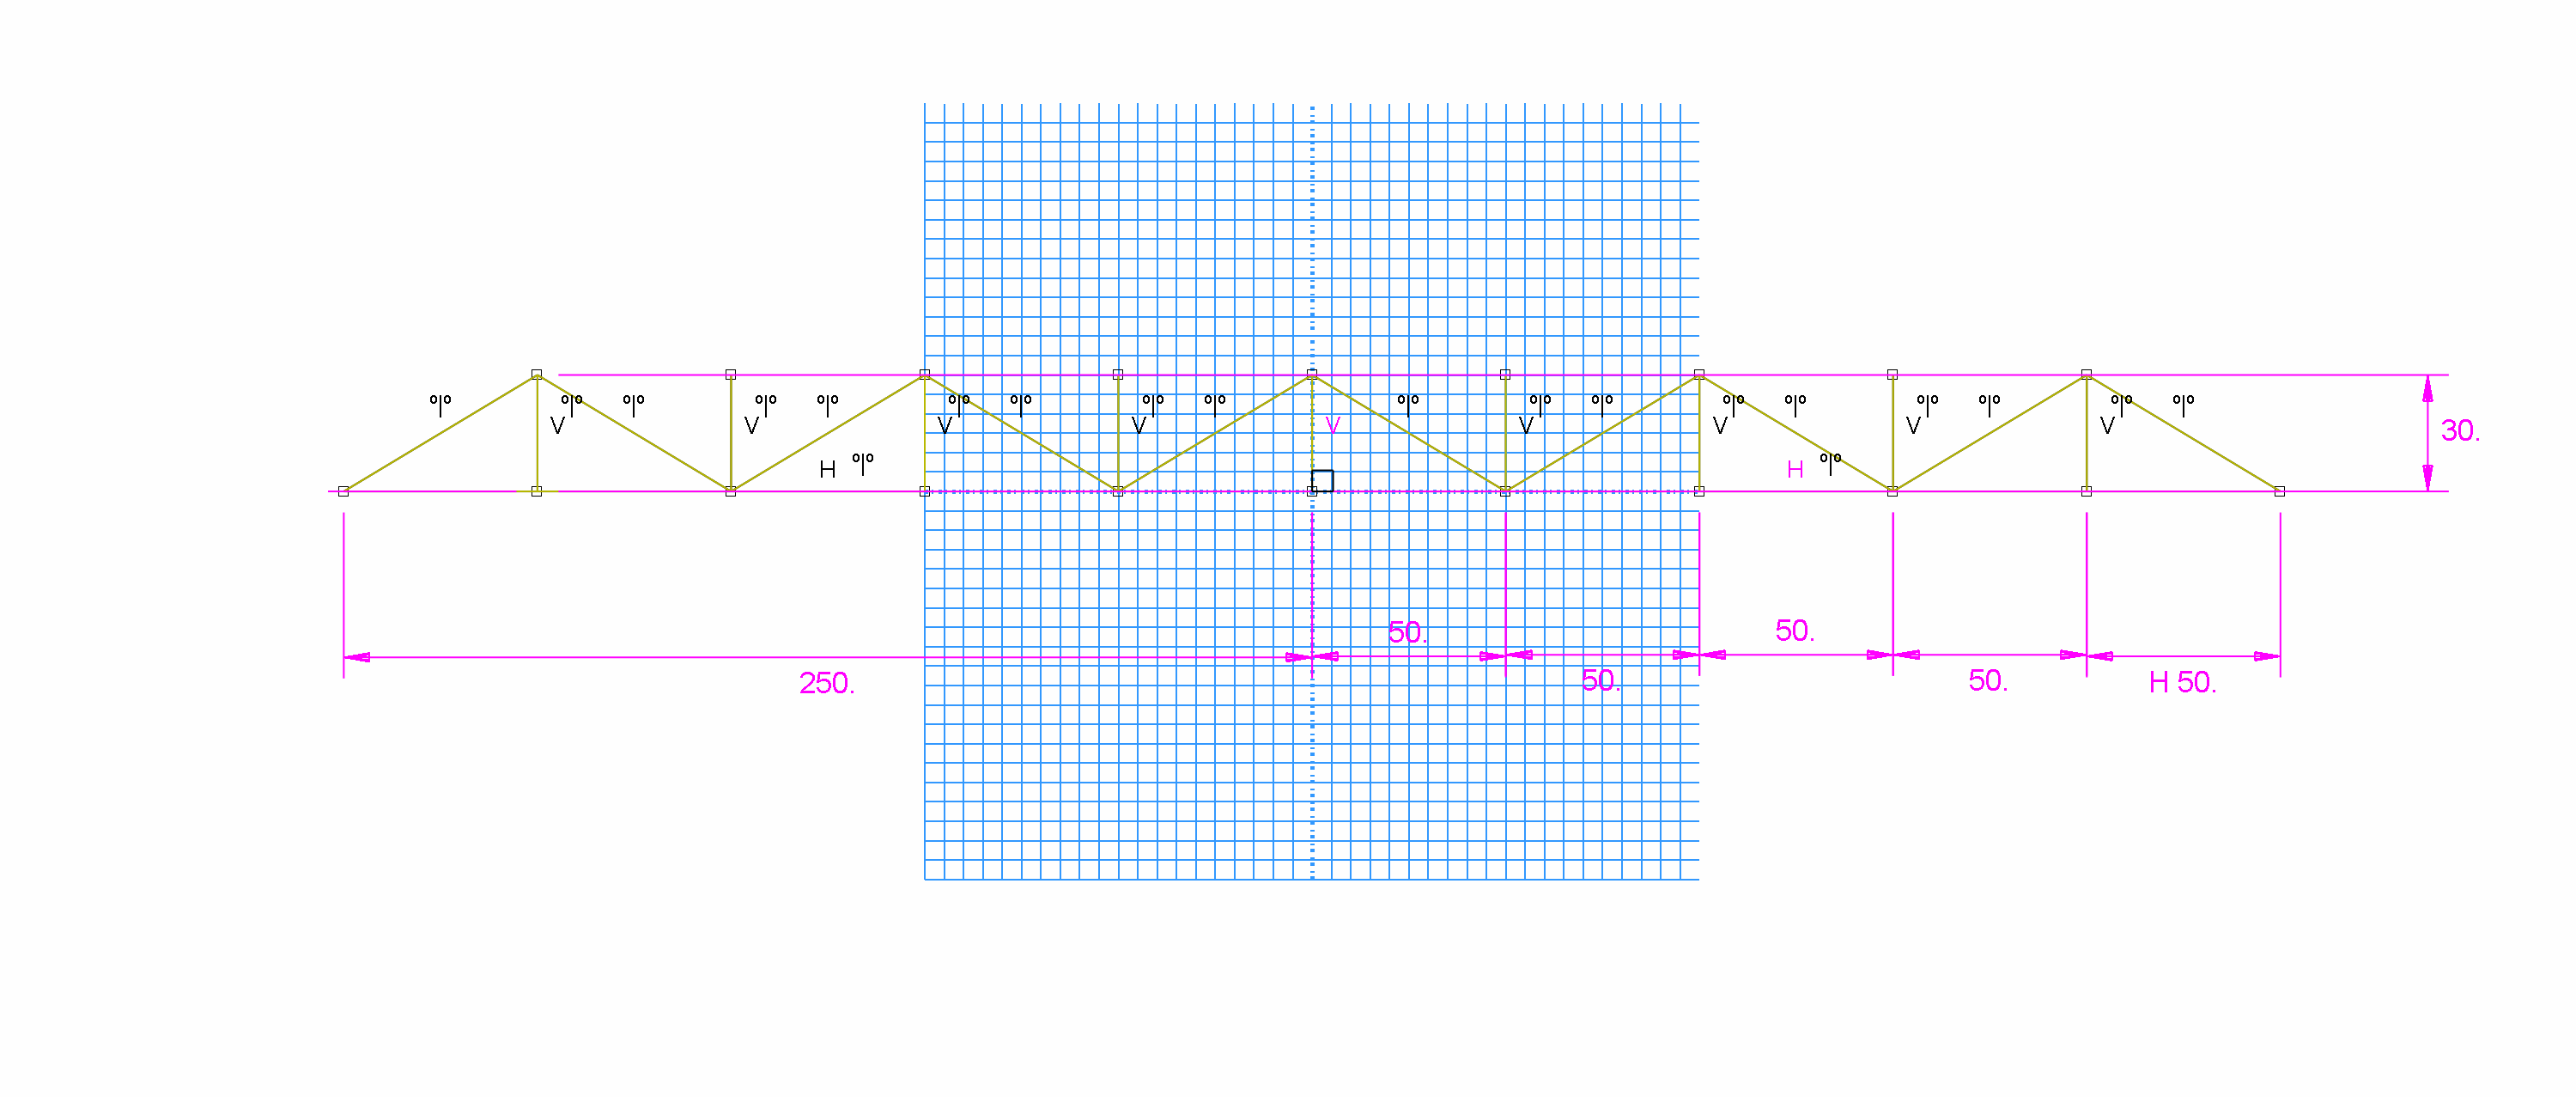
\includegraphics[width=0.6\textwidth]{04.png}
\end{center}

\textbf{钢缆}:

连接桥面与桥墩,共计2×2×5=20根。每根截面积为0.25。

采用杆单元建模

\begin{center}
\begin{tabular}{ll}
材料&:Steel\\
弹性模量&:117e9\\
泊松比&:0.266\\
密度&:7860\\
\end{tabular}
\end{center}

\subsection{Abaqus结果}

\begin{center}
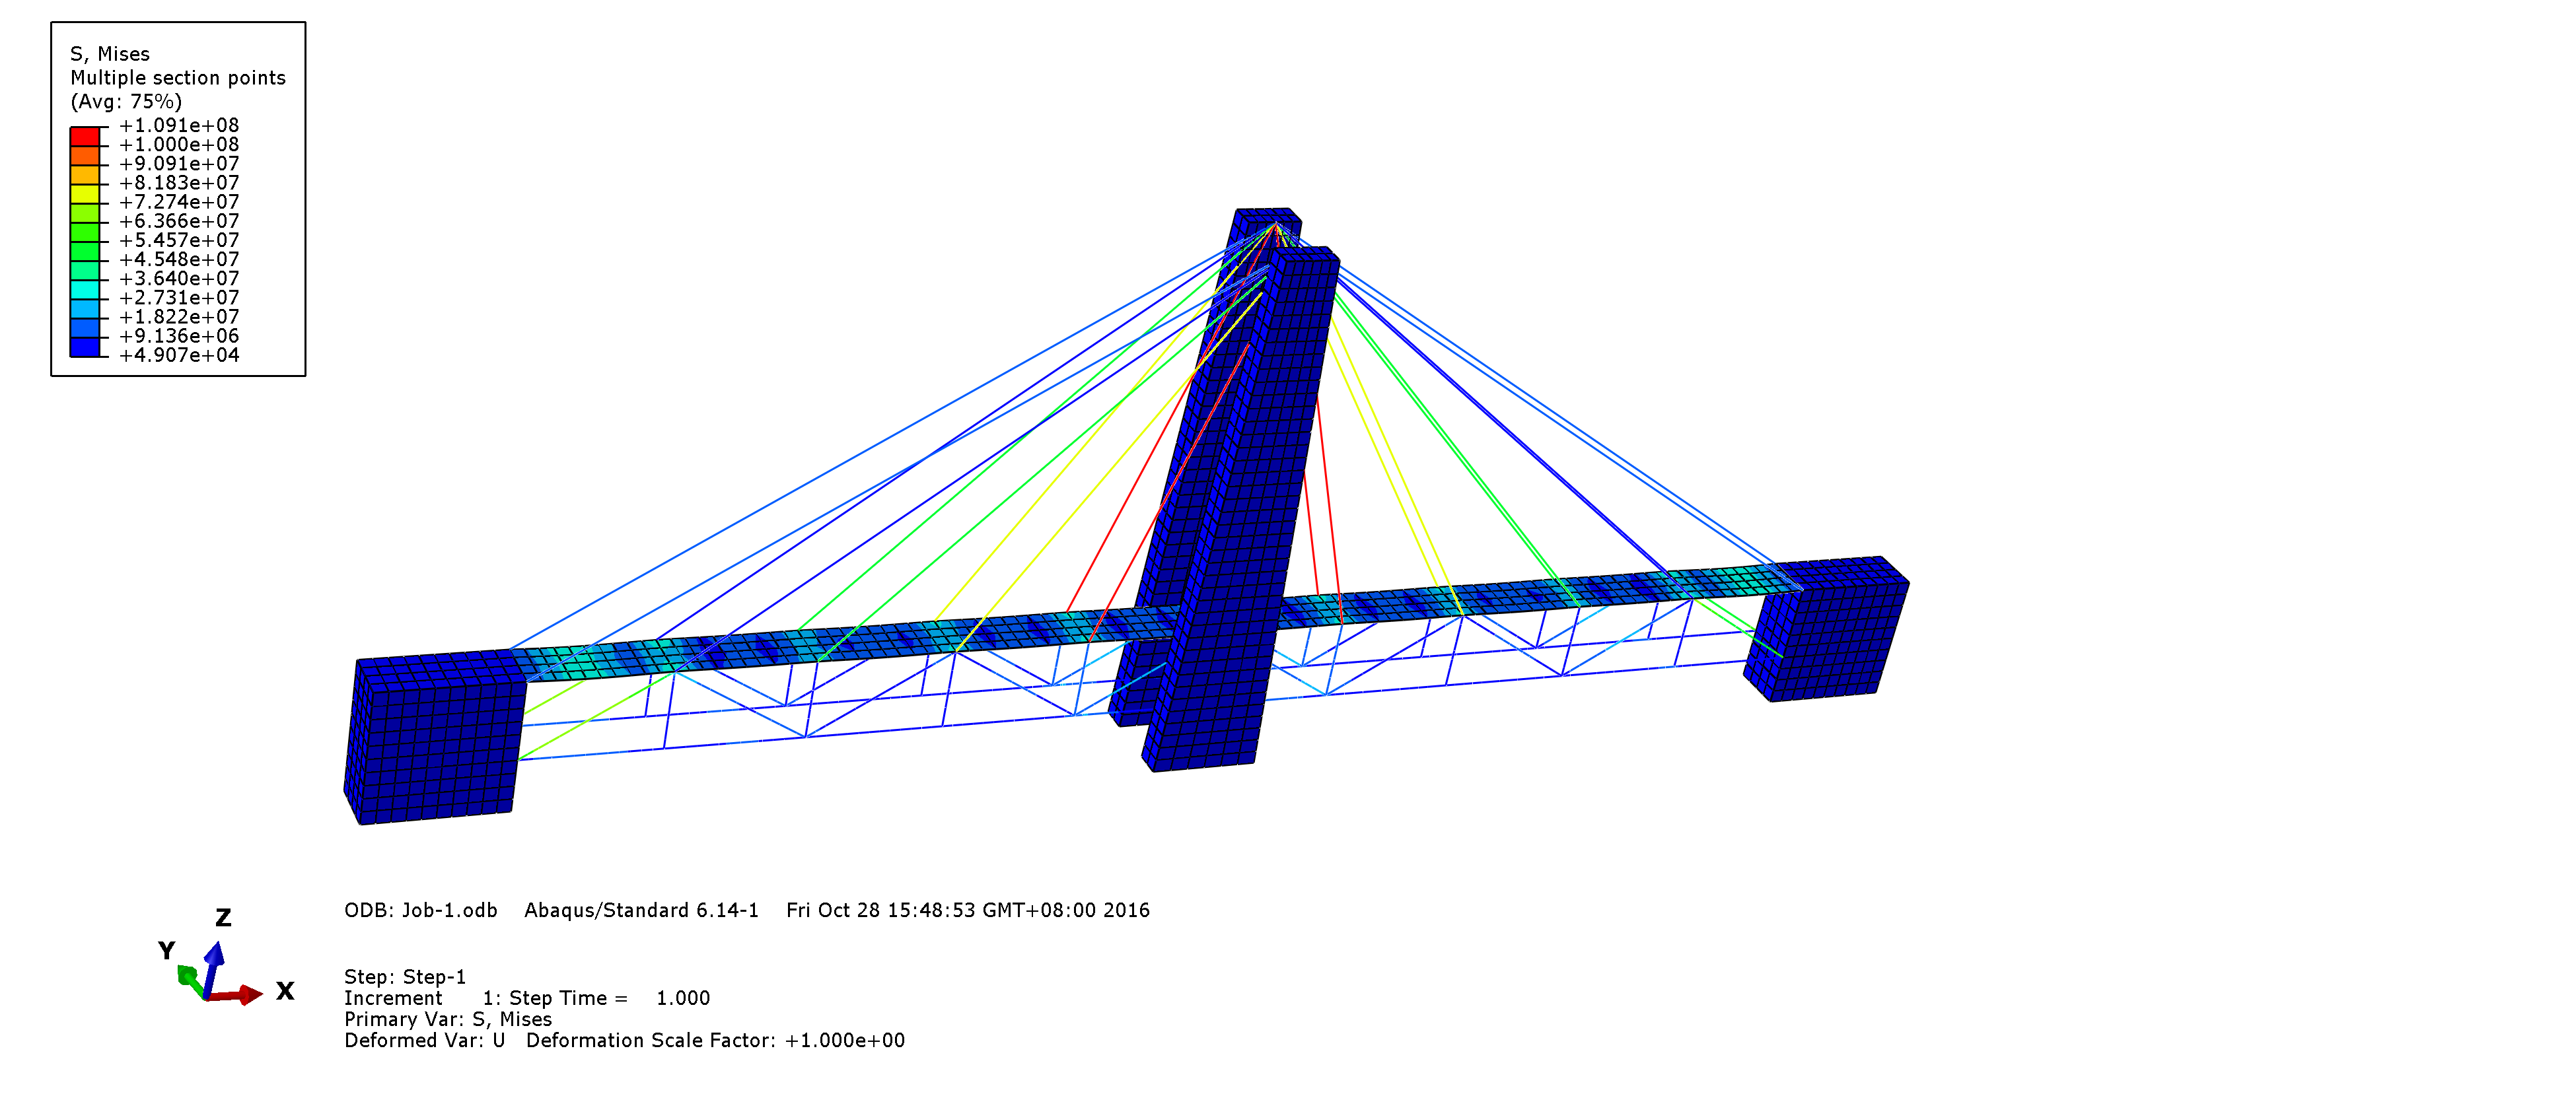
\includegraphics[width=0.6\textwidth]{05.png}
\end{center}


%-------------------------这里是各个部分的描述-------------------------------------
%----------------------------------------------------------------------------------
\section{桥梁功能实现方案}
\subsection{前处理}

前处理使用python与abaqus二次开发进行对INP文件的预处理,将其变成stap90能读入的标准文件。

\subsubsection{读入文件格式}
\textbf{功能开关}: 本小组采用的标准文件读入格式在规定的stap90固定格式基础上添加:
\begin{center}
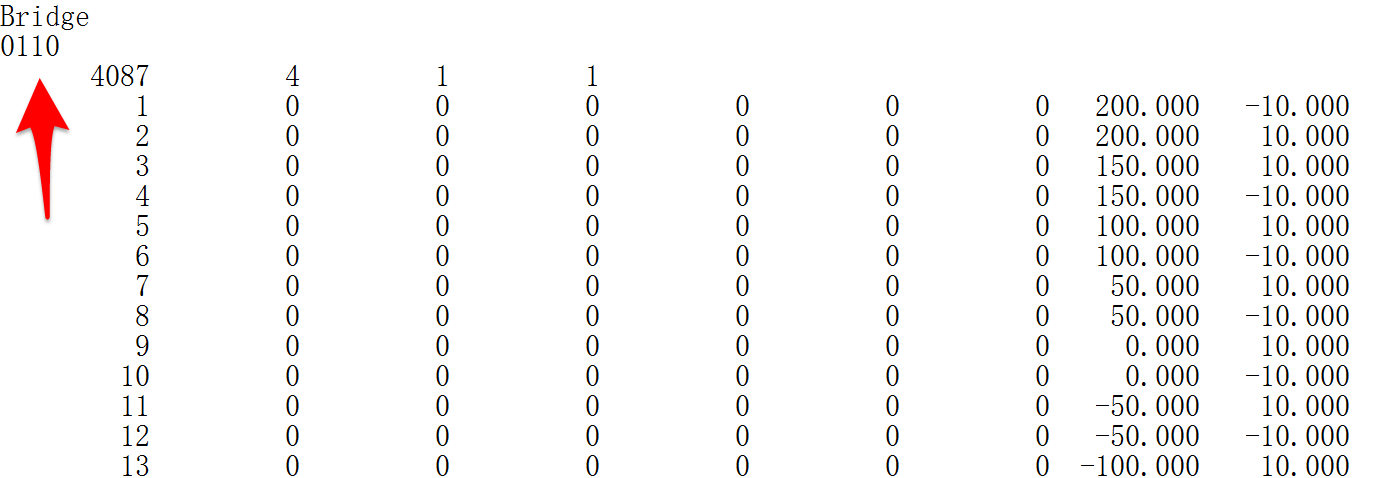
\includegraphics[width=\textwidth]{pre01.png}
\end{center}

对应的数字分别是以下功能开关:

BANDWIDTHOPT,PARDISODOOR,LOADANALYSIS,DYNANALYSIS,

\textbf{Pardiso}: 同时,我们需要在后面添加Pardiso所需的单元节点号(重复一遍)
\begin{center}
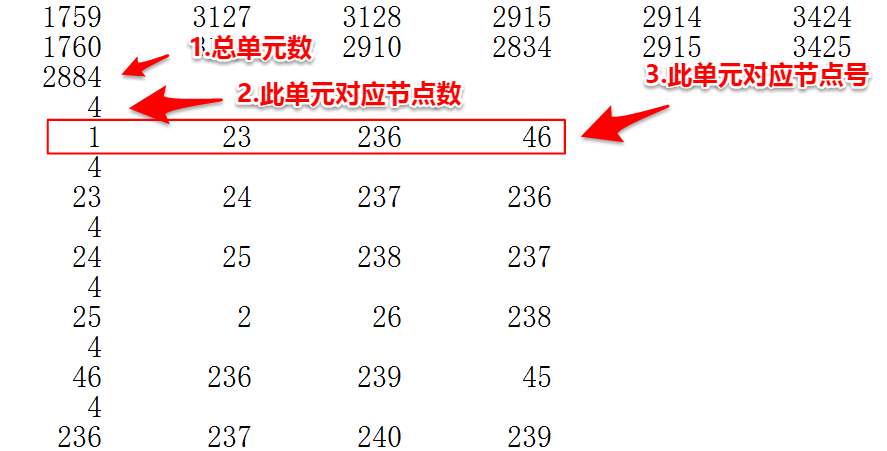
\includegraphics[width=\textwidth]{pre02.png}
\end{center}

\textbf{I10}: 为了求解大规模问题,我们将所有I5输入改为I10输入

\subsubsection{Python与abaqus二次开发}
以下三个步骤:
\begin{center}
\begin{tabular}{ll}
Mesh on part -- Mesh on instance\\
Merge Nodes\\
Renumber Nodes\\
\end{tabular}
\end{center}

前两者通过python完成,后一步直接可在abaqus操作:

1. mdb.models['Model-1'].setValues(noPartsInputFile=ON)

2. mdb.models['Model-1'].rootAssembly.InstanceFromBooleanMerge\\(name='PartMerge',instances=('Part-1-1','Part-2-1','Part-3-2','Part-3-2-lin-1-2'domain=MESH,mergeNodes=ALL)\\
(注:具体的models和name需要改成自己相对应的名字)

在abaqus也可操作merge命令

\begin{center}
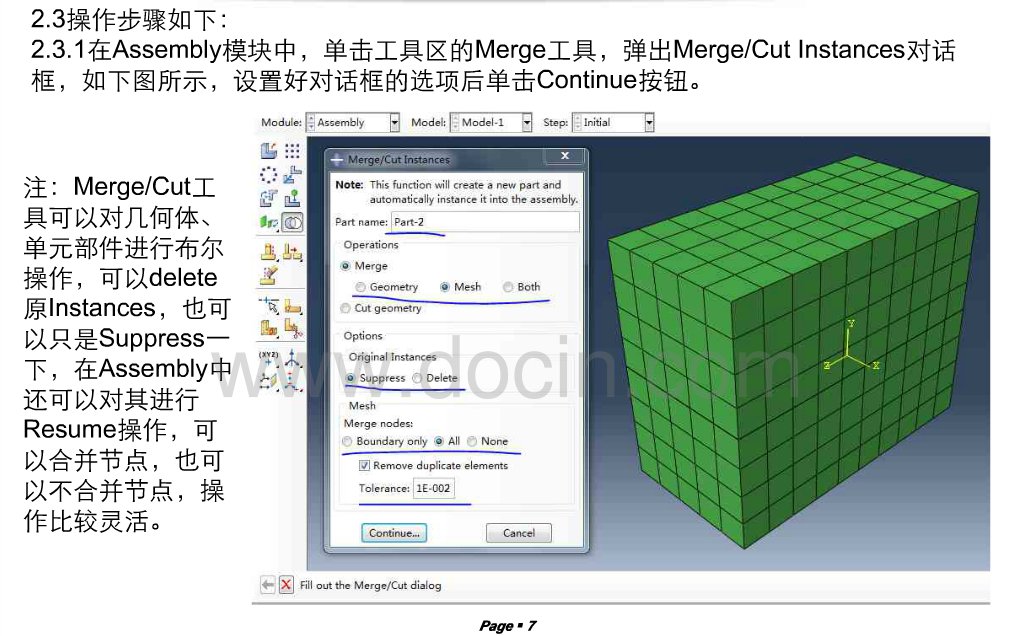
\includegraphics[width=\textwidth]{pre03.png}
\end{center}

3. 在abaqus中选择mesh,左栏功能最下面一个有对mesh操作的选项,选择renumber(注意需在mesh on part形式下,这就需要先按前两步生成所有instance变成一个part的操作)
\begin{center}
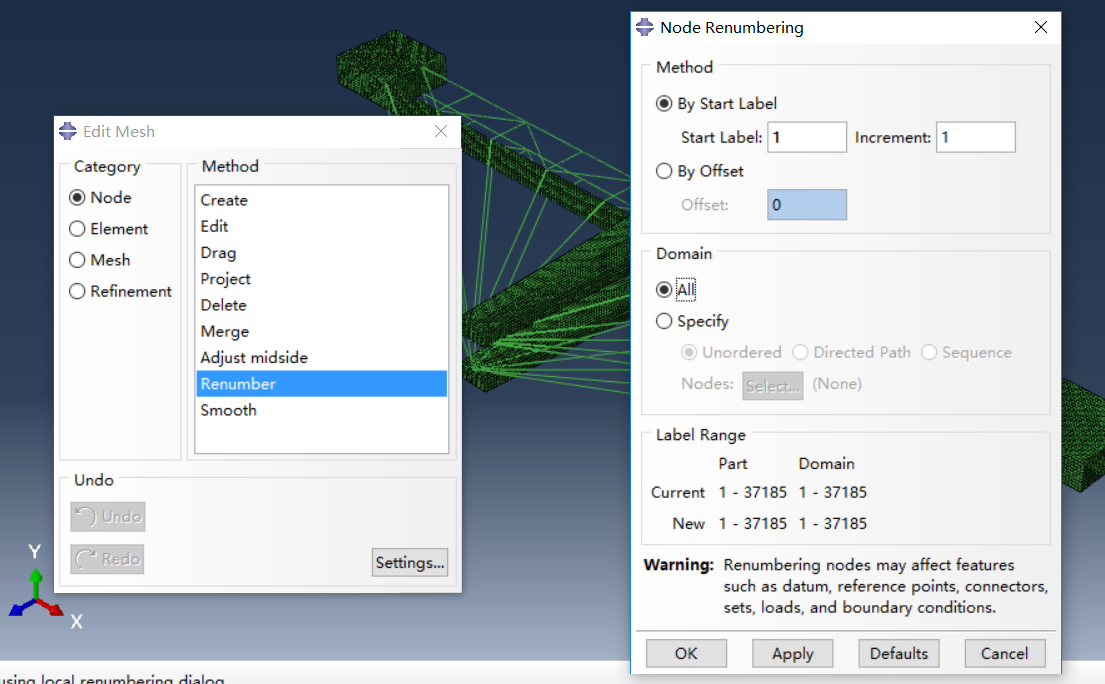
\includegraphics[width=\textwidth]{pre04.png}
\end{center}

前面三步分别生成merge-1文件,与merge-3文件,PreINP.py需要在相同的路径下找到这两个文件。

\subsubsection{PreINP.py实现}
基本原理就是,通过查找关键字来定位,其中具体的操作见PreINP.py源代码

\begin{center}
\includegraphics[width=\textwidth]{pre05.png}
\end{center}

%-----------------------------------------------------SPR----------------------------------------------%
\subsection{SPR}

采用SPR方法进行节点应力恢复。对于一个内部节点,若与8个8H单元相连,则有$n=8\times8=64$个高斯点用于应力恢复;对于一个边界面上的节点,则与4个单元相连,有32个高斯点用于应力恢复;同理,对于边界棱上的节点有16个,边界顶点上的节点有8个高斯点。为防止过拟合,对于边界面上的节点和内部节点采用二阶多项式进行最小二乘逼近,对于边界棱和边界顶点上的节点采用完备一阶多项式进行最小二乘逼近。以三维单元为例:
\begin{itemize}
\item 对二阶逼近:


\[
\boldsymbol{A}=\begin{bmatrix}1 & x_{1} & y_{1} & z_{1} & x_{1}y_{1} & y_{1}z_{1} & z_{1}x_{1}\\
1 & x_{2} & y_{2} & z_{2} & x_{2}y_{2} & y_{2}z_{2} & z_{2}x_{2}\\
\vdots & \vdots & \vdots & \vdots & \vdots & \vdots & \vdots\\
1 & x_{n} & y_{n} & z_{n} & x_{n}y_{n} & y_{n}z_{n} & z_{n}x_{n}
\end{bmatrix},\ \boldsymbol{X}=\begin{bmatrix}1 & x & y & z & xy & yz & zx\end{bmatrix}
\]



\[
\boldsymbol{C}_{ij}=\begin{bmatrix}c_{0} & c_{1} & c_{2} & c_{3} & c_{4} & c_{5} & c_{6}\end{bmatrix}^{T},\ \boldsymbol{S}_{ij}=\begin{bmatrix}\sigma_{ij}^{(1)} & \sigma_{ij}^{(2)} & \cdots & \sigma_{ij}^{(n)}\end{bmatrix}^{T}
\]



最小二乘逼近为解系数矩阵$\boldsymbol{C}_{ij}$,使得:$\boldsymbol{AC}_{ij}=\boldsymbol{S}_{ij},\ \text{即}\boldsymbol{A}^{T}\boldsymbol{AC}_{ij}=\boldsymbol{A}^{T}\boldsymbol{S}_{ij}$。最后解$\boldsymbol{X}^{(k)}\boldsymbol{C}_{ij}=S_{ij}^{(k)}$为第$k$个节点上的应力。

\item 对一阶逼近:


同理,但只取$1,\ x,\ y,\ z$的项使用。

\item 当连接到一个节点的所有单元具有的高斯点都不足以满足系数要求,或单元采用的为直接刚度法时,转而采用节点平均法恢复应力。这种情况常见于梁、杆、3T单元等。
\item 之前尝试过采用完备二阶多项式进行逼近,然而基本上都会出现过拟合现象。于是从逼近函数里删去平方项,得到的结果相对理想。
\item 算法分析

为得到每个节点对应的Patch,构建节点关系矩阵NodeRelationFlag,为NUMNP行矩阵,列数由单元类型以一般情况下够用来决定。对组内所有单元的连接矩阵作循环,除最后两列外,之前列按顺序存储循环得到的该节点连接的单元编号。倒数第二列指示该节点共连接的单元数,最后一列指示哪个单元的1号节点对应本节点,用于提取节点坐标。之后为按节点循环,得到所连接的单元的高斯点坐标及应力情况,对其按之前所述的方法进行最小二乘逼近,得到系数矩阵。最后根据系数矩阵和本节点的坐标得到本节点的应力情况。

\item 本程序对每一个单元组都采用这种思路进行节点应力恢复,并且按单元组顺序将包含节点的各应力分量输出至.OUT文件中
\end{itemize}

%---------------------------------------------------后处理--------------------------------------------------%
\subsection{后处理}
本程序后处理采用ParaView完成,在程序内包含输出为VTK文件的子程序VTKgenerate

在IND=0阶段,对VTK文件进行初始化,按VTK要求的格式写入文件头和各节点坐标。

在程序执行过程中,会将需要后处理而且要从内存中清除的数据写入3个临时文件中。分别为:

\begin{itemize}
\item $VTK.tmp$:存储位移和应力恢复信息,在WRITED(位移)和PostProcessor(应力)子程序处写入;
\item $VTKNode.tmp$:存储连接矩阵信息,在PostProcessor子程序处写入;
\item $VTKElTyp.tmp$:存储单元类型信息,在ElCal子程序处写入。
\end{itemize}

最后在IND=3阶段读取临时文件中的信息,按顺序整合为单一vtk格式的输出文件。网格形式为UNSTRUCTURED GRID,格式为ASCII,所记录的数据类型为double,包含三个场量:位移场、应力场和Von Mises应力场。以下为通过ParaView渲染生成的桥梁变形及应力分布及局部细节(变形放大倍率100,着色为Von Mises应力):
\begin{center}
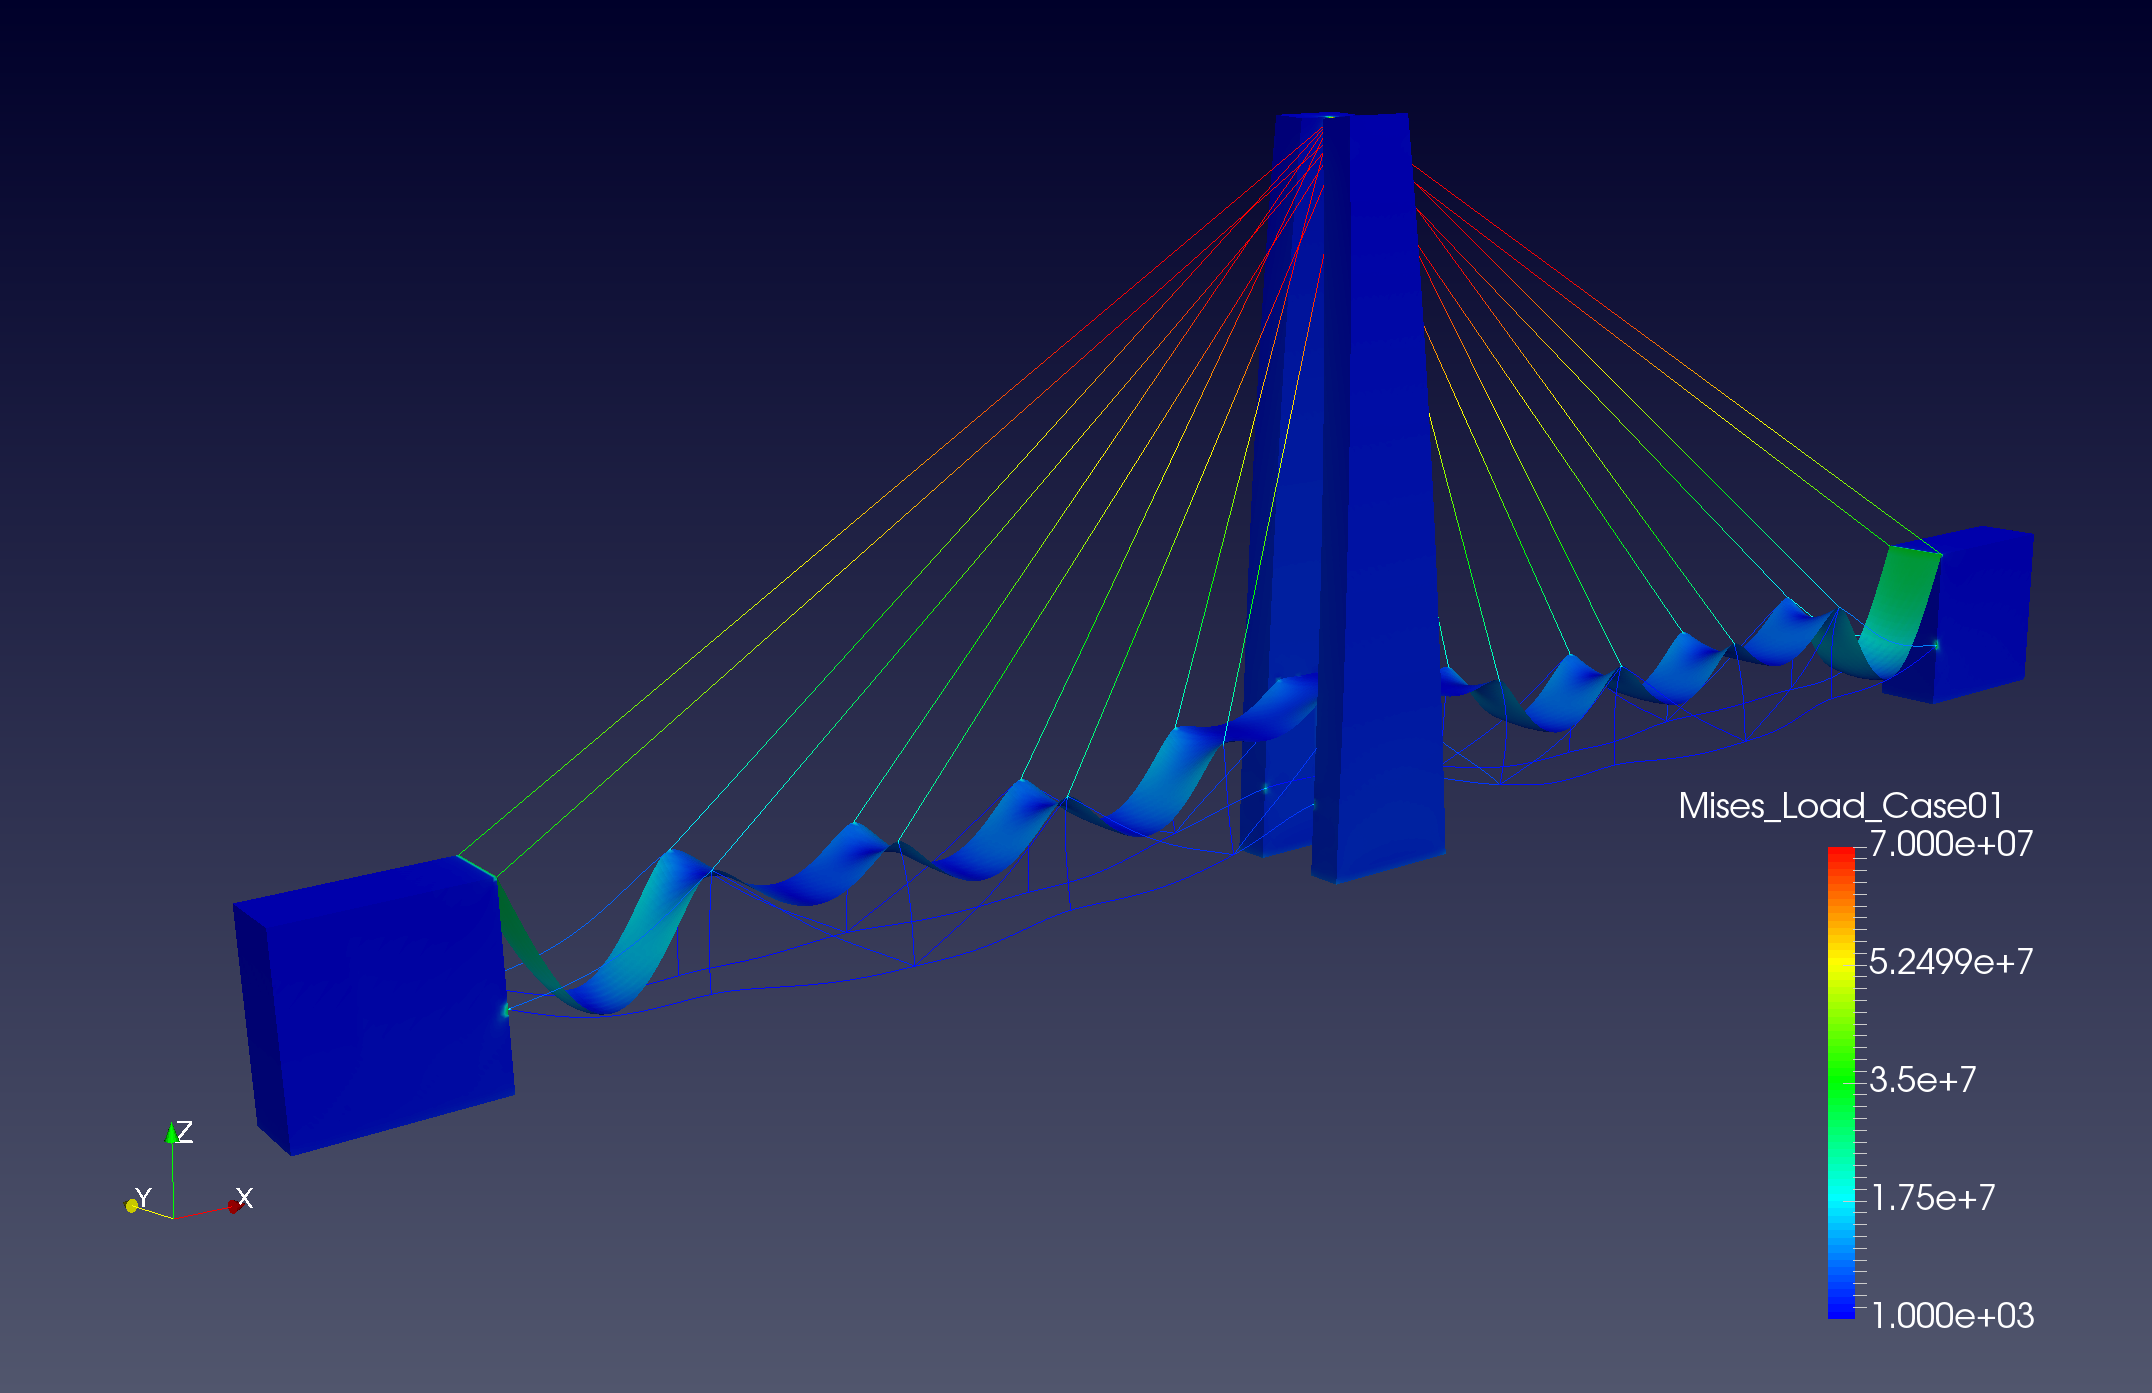
\includegraphics[width=0.8\textwidth]{Bridge-3.png}

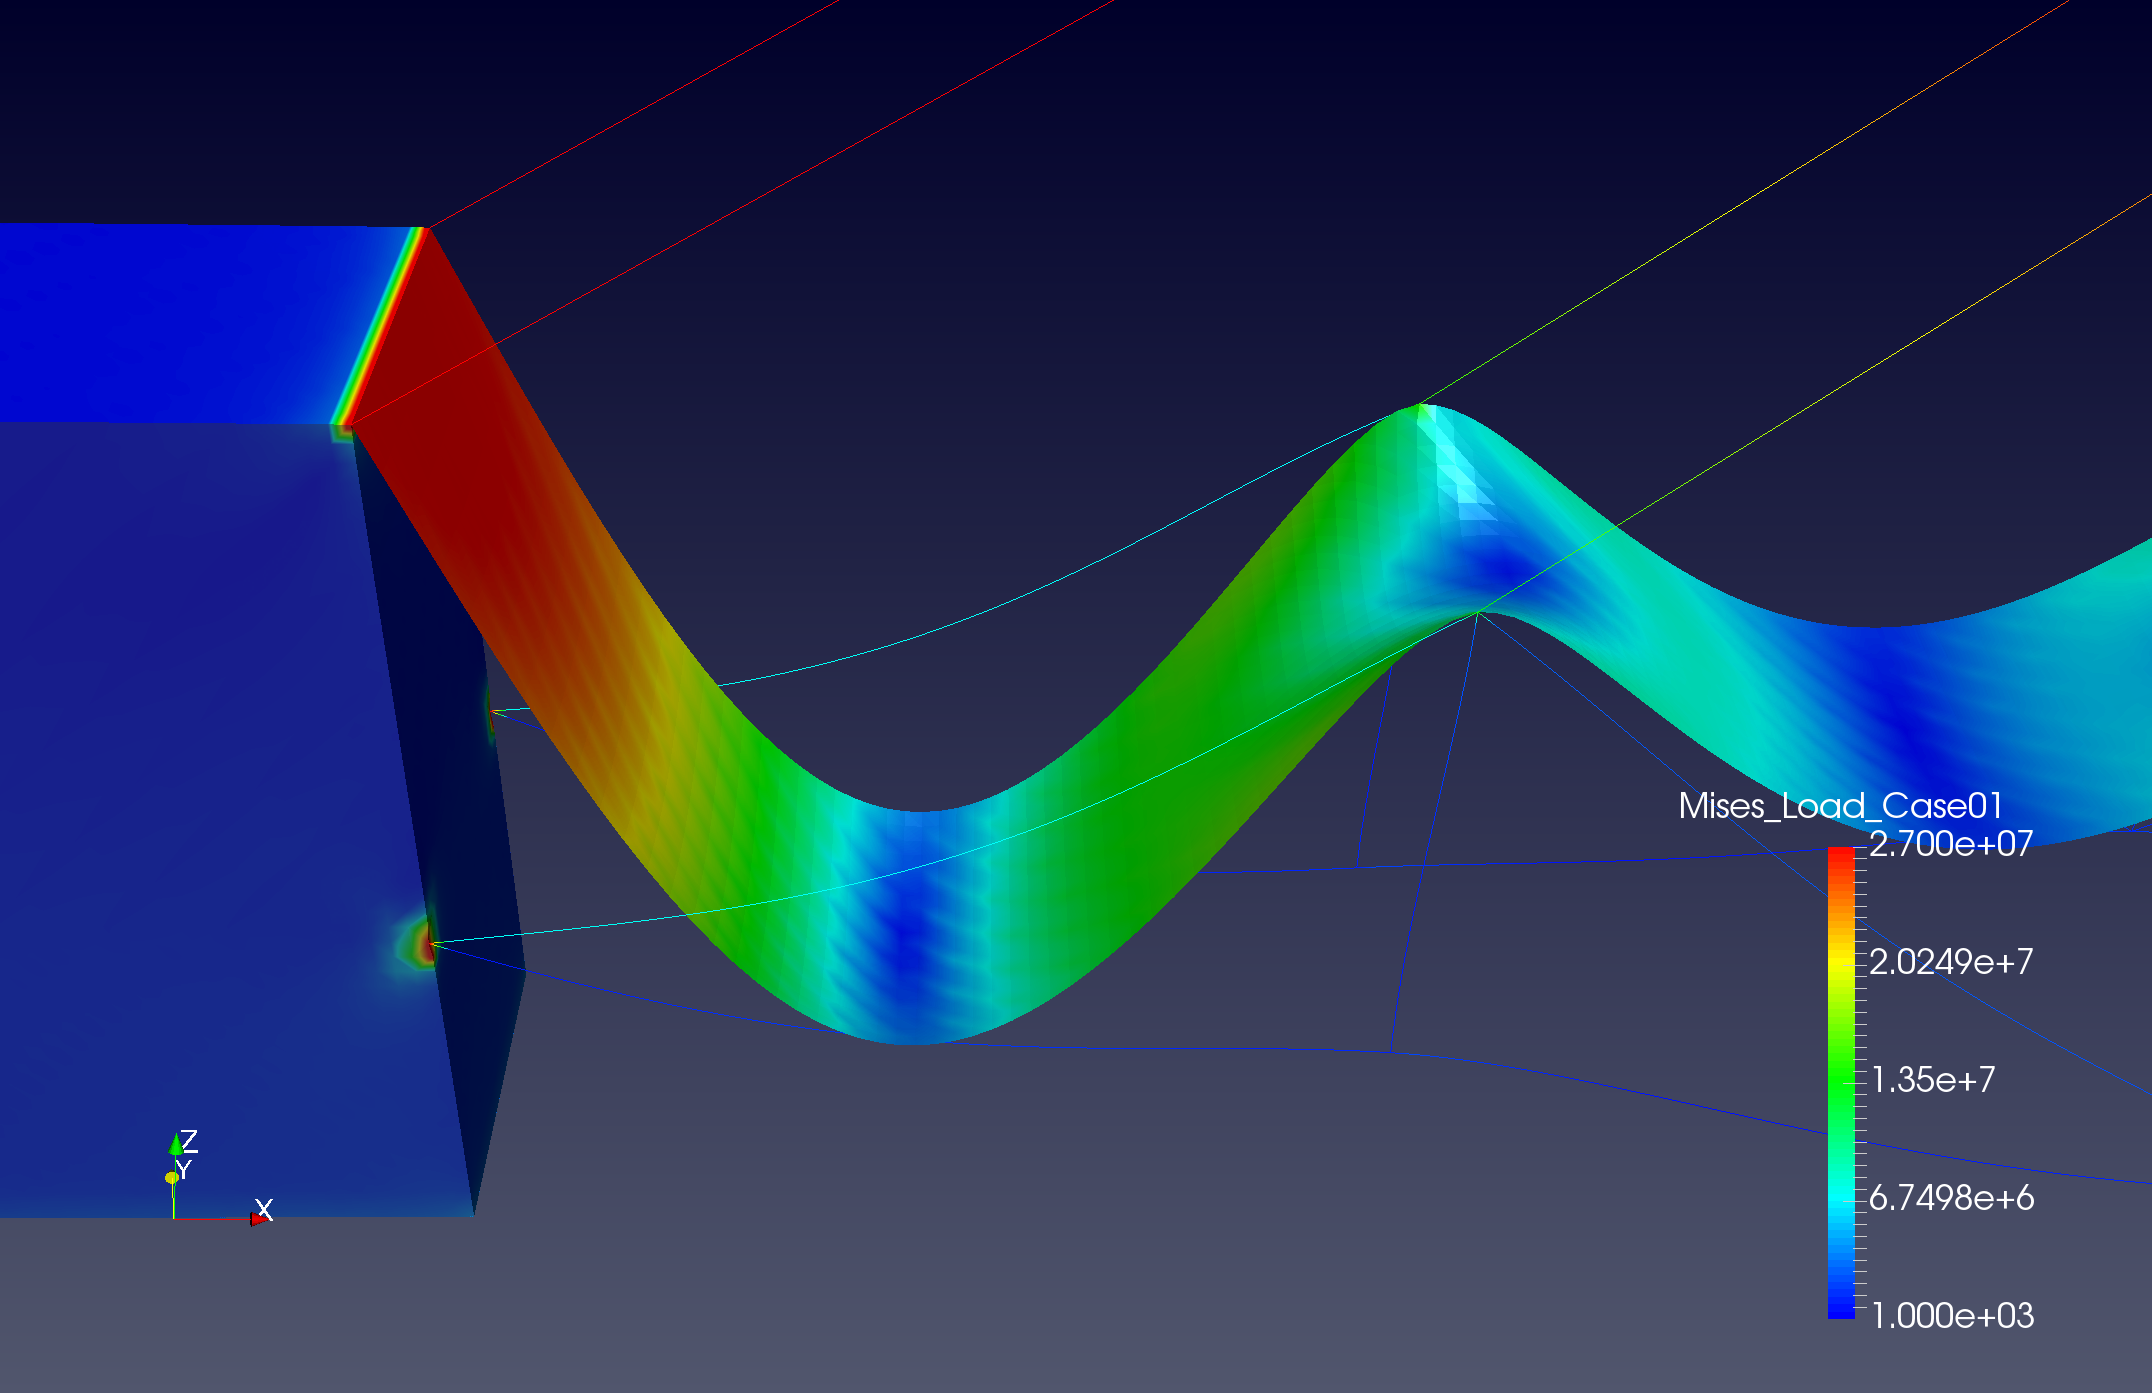
\includegraphics[width=0.8\textwidth]{Bridge-3-part.png}
\end{center}
%-------------------------------------------------------8H--------------------------------------------------%
\subsection{8H}

\begin{itemize}
\item 算法分析

给出一个8H单元,其节点坐标矩阵为$\boldsymbol{X}=\begin{bmatrix}x_{1} & y_{1} & z_{1}\\
x_{2} & y_{2} & z_{2}\\
\vdots & \vdots & \vdots\\
x_{8} & y_{8} & z_{8}
\end{bmatrix}$,每条边的方向上采用2点高斯积分,共8个高斯点,并采用三线性函数作为形函数。作前处理时,将坐标变换到$\xi,\ \eta,\ \zeta$下求形函数的梯度,再对8个高斯点作加权求和,得到单元刚度阵:


\[
N_{i}=\frac{1}{8}(1+\xi_{i}\xi)(1+\eta_{i}\eta)(1+\zeta_{i}\zeta),\ i=1,2,...,8
\]
\[
\boldsymbol{N}=\begin{bmatrix}\boldsymbol{N}_{1} & \boldsymbol{N}_{2} & \boldsymbol{N}_{3} & \boldsymbol{N}_{4} & \boldsymbol{N}_{5} & \boldsymbol{N}_{6} & \boldsymbol{N}_{7} & \boldsymbol{N}_{8}\end{bmatrix},\ \boldsymbol{N}_{i}=N_{i}\begin{bmatrix}1\\
 & 1\\
 &  & 1
\end{bmatrix}
\]
\[
GN=\begin{bmatrix}\frac{\partial N_{1}}{\partial\xi} & \frac{\partial N_{2}}{\partial\xi} & \cdots & \frac{\partial N_{8}}{\partial\xi}\\
\frac{\partial N_{1}}{\partial\eta} & \frac{\partial N_{2}}{\partial\eta} & \cdots & \frac{\partial N_{8}}{\partial\eta}\\
\frac{\partial N_{1}}{\partial\zeta} & \frac{\partial N_{2}}{\partial\zeta} & \cdots & \frac{\partial N_{8}}{\partial\zeta}
\end{bmatrix}
\]



\[
\boldsymbol{B}=\nabla_{s}\boldsymbol{N}=\begin{bmatrix}\boldsymbol{B}_{1} & \boldsymbol{B}_{2} & \boldsymbol{B}_{3} & \boldsymbol{B}_{4} & \boldsymbol{B}_{5} & \boldsymbol{B}_{6} & \boldsymbol{B}_{7} & \boldsymbol{B}_{8}\end{bmatrix},\ \boldsymbol{B}_{i}=\begin{bmatrix}B_{ix} & 0 & 0\\
0 & B_{iy} & 0\\
0 & 0 & B_{iz}\\
B_{iy} & B_{ix} & 0\\
0 & B_{iz} & B_{iy}\\
B_{iz} & 0 & B_{ix}
\end{bmatrix},\ i=1,2,...,8
\]



$\boldsymbol{B}$矩阵的各量由单元Jacobian矩阵和形函数对各坐标的导数得到:


\[
\boldsymbol{J}^{-1}\cdot GN=\begin{bmatrix}B_{1x} & B_{2x} & \cdots & B_{8x}\\
B_{1y} & B_{2y} & \cdots & B_{8y}\\
B_{1z} & B_{2z} & \cdots & B_{8z}
\end{bmatrix},\ \boldsymbol{J}=GN\cdot\boldsymbol{X}^{T}
\]



$\boldsymbol{D}$矩阵由本构关系得到,在此认为材料是各向同性的:


\[
\sigma_{ij}=2G\varepsilon_{ij}+\lambda\varepsilon_{kk}\delta_{ij}
\]
$\Rightarrow\boldsymbol{D}=\begin{bmatrix}2G+\lambda & \lambda & \lambda\\
\lambda & 2G+\lambda & \lambda\\
\lambda & \lambda & 2G+\lambda\\
 &  &  & 2G\\
 &  &  &  & 2G\\
 &  &  &  &  & 2G
\end{bmatrix},\ \text{s.t. }\boldsymbol{\sigma}=\boldsymbol{D\varepsilon},\ \text{where }\boldsymbol{\varepsilon}=\begin{bmatrix}\varepsilon_{x}\\
\varepsilon_{y}\\
\varepsilon_{z}\\
\varepsilon_{xy}\\
\varepsilon_{yz}\\
\varepsilon_{zx}
\end{bmatrix},\ \boldsymbol{\sigma}=\begin{bmatrix}\sigma_{x}\\
\sigma_{y}\\
\sigma_{z}\\
\tau_{xy}\\
\tau_{yz}\\
\tau_{zx}
\end{bmatrix}$.


\[
\boldsymbol{K}^{e}=\sum_{i=1}^{2}\sum_{j=1}^{2}\sum_{k=1}^{2}w_{i}w_{j}w_{k}\boldsymbol{B}^{T}(\xi_{i},\eta_{j},\zeta_{k})\boldsymbol{DB}(\xi_{i},\eta_{j},\zeta_{k})
\]



生成单元刚度阵通过Location Matrix进行组装,得到全局的刚度阵,再解$\boldsymbol{Kd=f}$.


\item 算法实现


位移计算部分按照变换将坐标变换到$[-1,1]\times[-1,1]\times[-1,1]$后即可得到形函数和各导数。取得高斯点位置,代入$\boldsymbol{D}$矩阵即可以产生单元刚度阵,调用COLHT和ADDBAN生成总刚度矩阵并求解。


SPR部分,在前处理时保存单元连接矩阵到临时文件中,在后处理中调取,计算每个节点连接的单元数量和编号,以及用于恢复节点位置的信息,生成为NodeRelationFlag数组。对每个节点,根据该数组选取逼近的阶次,计算$\boldsymbol{A}\text{、}\boldsymbol{S}$矩阵,并传入最小二乘子程序LeastSquare中,得到系数数组,并代入节点位置信息,得到恢复的节点应力。

\item 算法测试


Patch Test 选取了7单元模型和8单元模型进行测试,测试形状为单位立方体,$E=1000,\ \nu=0.25$,通过内部确定1个或8个点来将其分划为8个或7个单元。施加线性位移场:


\[
u_{x}=0.001x,\ u_{y}=0.002y,\ u_{z}=0.003z
\]



得到各点需要施加的外力,并采用最少的边界条件对单元进行测试。测试结果如 data/8H 中各输入输出文件所示。


测试结果表明,对于线性场,输出误差在机器$\varepsilon$量级,单元设计能精确重构线性位移场,为一阶收敛的。


对SPR的测试,其输出结果误差也在机器$\varepsilon$量级,因而从算法设计的角度来说是合理的。




\end{itemize}


\subsection{Beam}
\subsubsection{Basic principles}
\paragraph{}
For a beam element, the equation for a single beam element is quite simple, for the reason that the calculation of the element stiffness matrix doesn't require numerical integral.It can be done manually.
The stiffness matrix for a beam element is as follow.
\begin{center}
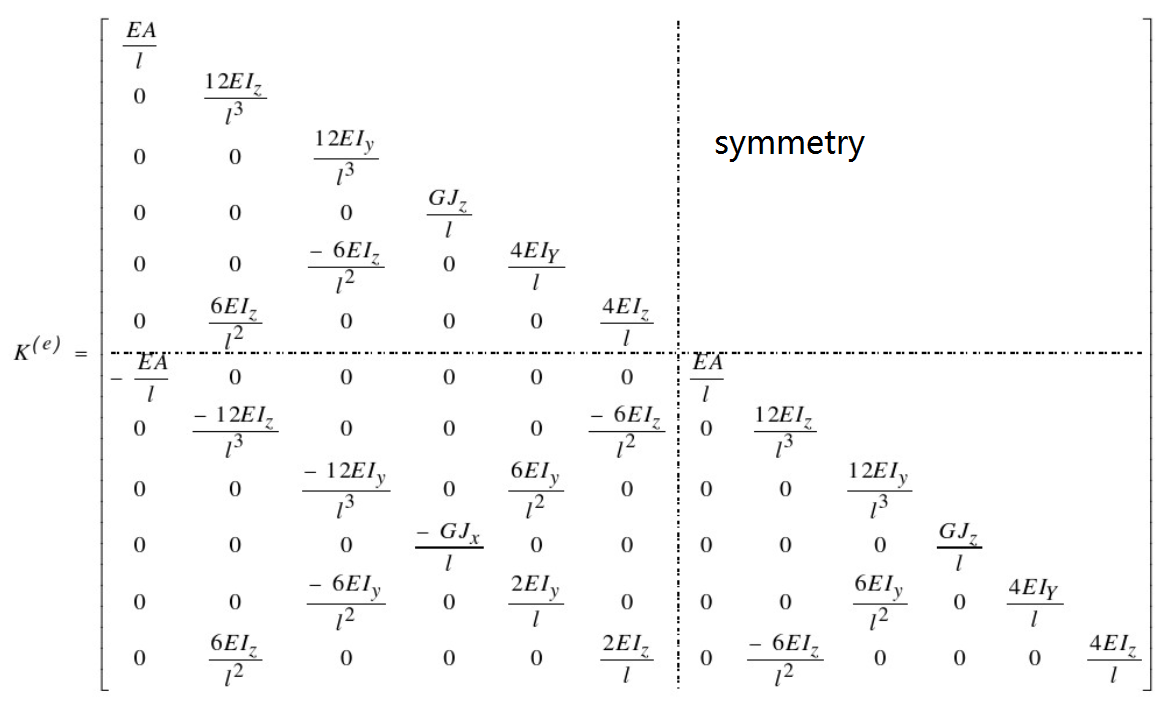
\includegraphics[width=1.0\textwidth]{beam1.png}
\end{center}
\begin{center}
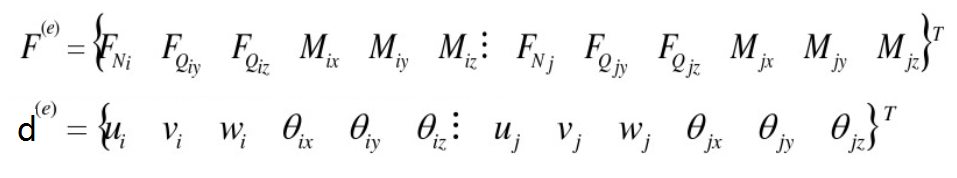
\includegraphics[width=1.0\textwidth]{beam2.png}
\end{center}
In all, we can get the equation for the element itself.
\begin{equation}
{\bf K^{(e)}d^{(e)}=F^{(e)}}
\end{equation}
The process of assembly and solution of the linear equation is just the same as the former elements.
\paragraph{ATTENTION} The stiffness matrix for beams point to arbitrary directions needs the translation matrix to do the coordinates translation.
\begin{equation}
{\bf K^{(e)\prime}=T^{T}K^{(e)}T}
\end{equation}
\subsubsection{Programming procedures}
\paragraph{}
The most difficult part for the programming is the generation of the ID array without interfering with other elements. The structure of the STAP90 program is very terrible for this kind of modification, given the reason that the original program read the element controlling messages after the nodes, making it complex for the dealt for nodes. The only choice left for me is whether changing the whole blueprint for the entire STAP 90 program or just writing the individual input or output subroutine for  the beam. In terms of the deadline requirements, I choose the lateral,leaving the former mission to the following weeks. As you can see in the source files, the input and output subroutine for the beam is in the 'BEAM.f90'.
\subsubsection{Input file format}
\paragraph{}For controlling messages of nodals:
\begin{center}
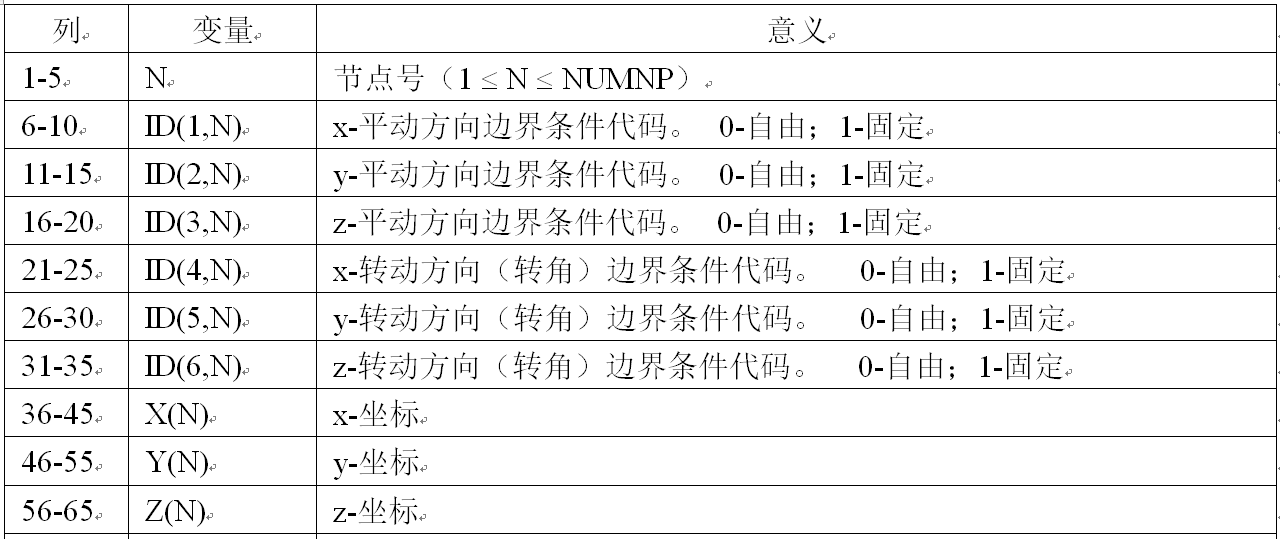
\includegraphics[width=1.0\textwidth]{beam3.png}
\end{center}
\paragraph{}For information about the loads:
\begin{center}
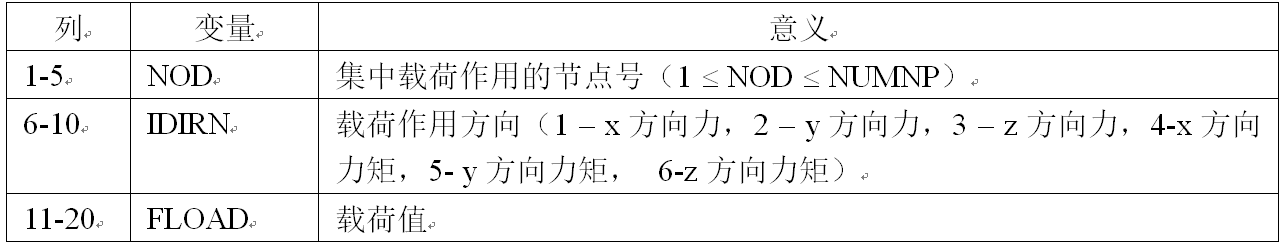
\includegraphics[width=1.0\textwidth]{beam4.png}
\end{center}
\paragraph{}For information about the materials:
\begin{center}
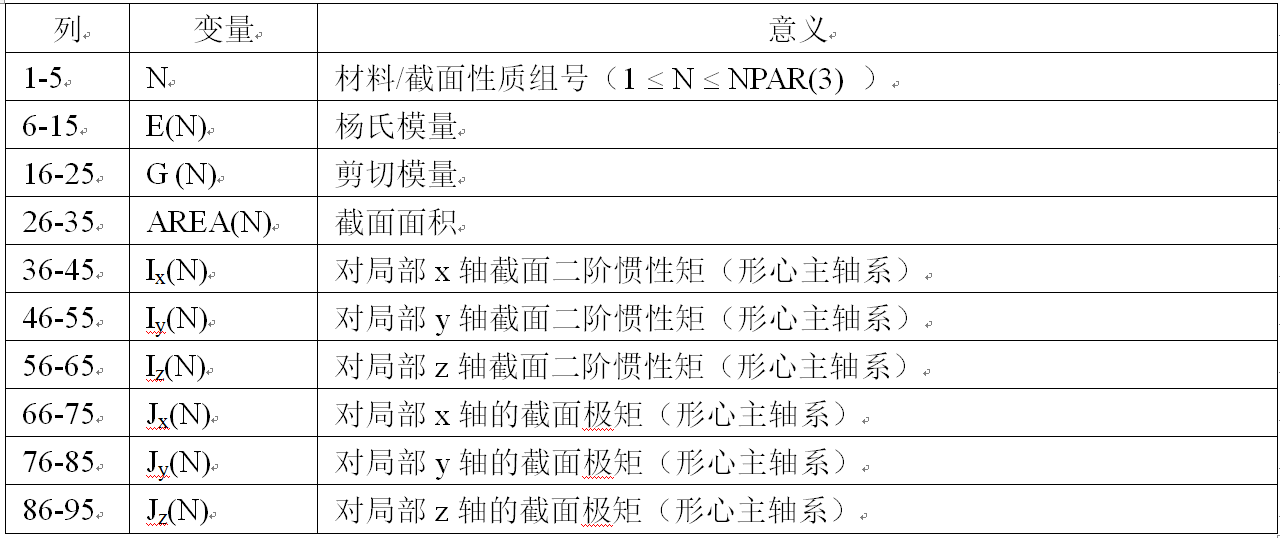
\includegraphics[width=1.0\textwidth]{beam5.png}
\end{center}
\paragraph{}For information about the element connectivity:
\begin{center}
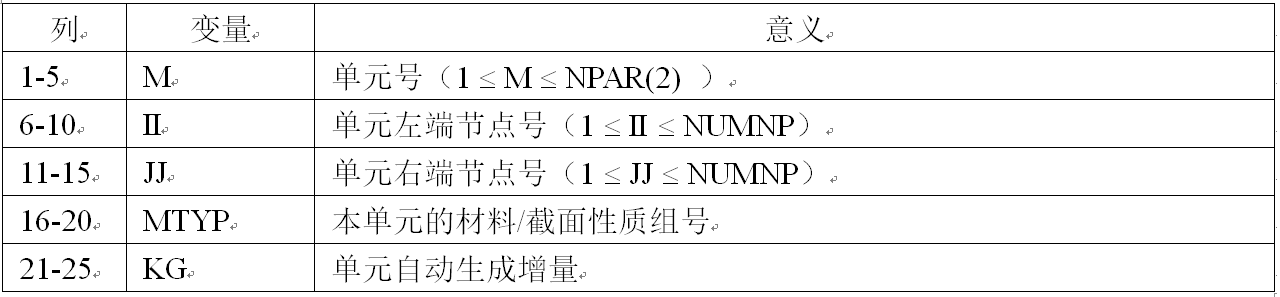
\includegraphics[width=1.0\textwidth]{beam6.png}
\end{center}
\subsubsection{The rate of convergence}
For the beam, the FEM guarantees the continuity and the completeness. The completeness will be verified in the patchtest.For continuity, the method for the approximation of the function is 3-order Hermite interpolation, maintaining the continuity for both the displacement and the angle.It is obvious that the FEM will give the exact answer at nodes if we give concentration forces or momentum at the nodes.For the distribution forces, the FEM will not give the exact results. The reason for this is that the order of the moment is at least 2 for the distribution forces. The results will be better and will converge to the exact solution with the mesh refined to infinite decimal.The convergence rate for the displacement is at the order of 2, while the rate for the energy norm is at the order of 1.
\subsubsection{Patchtest and the results}
I use an example for the patchtest.The situation of the load and the structure is as follow.
\begin{center}
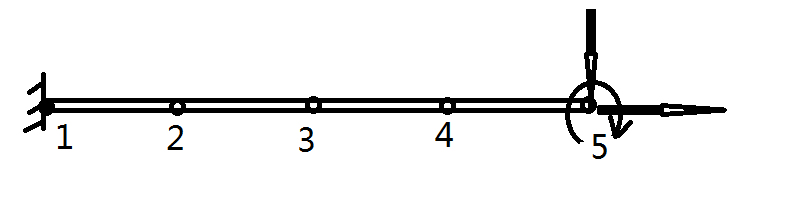
\includegraphics[width=1.0\textwidth]{beam7.png}
\end{center}
The input files and the results for the patchtest in the folder for the beam.
\subsection{Shell}

\subsection{半带宽优化}

\subsubsection{简介}
首先需要注意的是,半带宽优化已经被证明是一个NP完全问题,所以无法在多项式时间得到最优解。现在的算法主要是近似的优化算法,目前主流的算法有CM算法,GPS算法,tabu搜索算法,GRASP算法,模拟冷却算法等。
由于程序的最初设计以速度优先,故在选择的时候排除了耗时巨大的模拟冷却算法,而是采用了偏于经验类的算法。加之使用FORTRAN语言实现图结构困难,所以半带宽部分选择在stap90程序中实现最为原始的CM算法。而对于更加强力一点的算法,则选择用$C++$予以实现GRASP算法的部分。
\paragraph{算法介绍}
a)CM算法\\
CM算法全称Cuthill-McKee算法在这两人于1969年名为Reducing the bandwidth of sparse symmetric matrices的论文中提出,是最先被提出的半带宽优化算法。其主要实现较为简单,主要就是通过一个广度优先搜索,每次把入度最小的点标号,并把该点的邻居加入队列中,通过循环得到最终的编号。\\
b)GRASP算法\\
GRASP算法是在2004年由西班牙Valencia大学的Estefania Piñana教授等人在其文章GRASP and path relinking for matrix bandwidth minimization中提出的。其吸取了前人(CM, GPS, Tabu)的优点,在试验中有着非常优秀的表现。
其主要内容分为三个阶段,构建阶段,提升阶段和路径重连阶段。
构建阶段提出了5中不同的方案,在保证优质初始解的同时也考虑了其随机性,避免其落入局部最优点。在大作业的$C++$部分实现中,我才用了C1部分,主要原因还是比较易于操作。
提升阶段参考于tabu算法的交换节点编号的部分,不过为了提升性能,GRASP算法仅仅考虑在交换时会改变最大带宽以及最大带宽点的个数的点。
路径重连部分适用于极大规模问题,而且需要有多局部极值,并不适用于本问题,故忽略。
\subsubsection{算法实现}
在stap90中,如果要使用半带宽优化,为了简便操作,我选择了在输入文件中加入部分信息,也就是在输入ID之后就输入整体的连接矩阵。再次说明一下这一点的必要性,因为半带宽优化关心的是图的整体结构,所以整体的连接矩阵必不可少,而新产生的ID矩阵又必须在组装过程中发挥作用,所以选择了在输入原先的ID之后直接输入连接矩阵。
在具体实现中,因为FORTRAN没有可变数组的支持,我先是构建了一个node模板和一个list模板,具体接口请详见list.f90与node.f90。通过循环将与自由度i有关的所有自由度都放在了链表数组lists(i)之中,然而由于链表的搜索功能是其软肋,所以在实现搜索的时候还是比较麻烦的。
而$C++$的部分则是比较轻松,同时实现了类似的接口完成了算法实现。
Stap90的实现位于$solvermode.f90$文件中的bdopt函数,C++的实现位于BandwidthOpt文件夹中。
\paragraph{}
在实验中,我发现由于决定skyline算法时间的主要因素是nwk,也就是skyline存贮中的元素个数,而不是最大带宽,加上桥问题的主要问题在于其部分元素带宽很大,而大多数很小,导致使用了优化虽然可以使带宽从1492降至1356,但是总元素个数增加,时间反而从12s增长至18s,得不偿失。这说明半带宽优化并不适用于所有问题。

\subsection{稀疏存储求解器}
\subsubsection{简介}
首先对稀疏矩阵进行一些简单介绍。
稀疏矩阵主要指非零元素为O(n)的矩阵。其没有必要使用以往的$O(n^2)$求解,而是可以利用特殊的储存方式,大大缩减存储空间。与此同时,因为实际上的计算大多仅仅与非零元素有关,所以有算法可以将求解线性方程$Lx=y$的时间降至O(flop)(其中flop为非零元素个数)大大降低其运算时间,是求解有稀疏性质的线性系统的一把利器。
本次采用intel MKL中集成的pardiso求解器,因为其为市面上速度最快的求解器。矩阵的存储方式采用默认的CSC格式。值得一提的是,相比于stap90中原有的skyline求解器,pardiso在空间上有着劣势。因为skyline求解器可以在原地进行$L^TDL$分解,而CSC存储的矩阵,由于不知道分解后非零元素的位置,需要在过程中被迫开一份$O(n^2)$的空间。
\subsubsection{实现}
由于具体的函数调用都是相同的MKL中的pardiso,所以实现中更重要的是一些小细节,而这些小细节就是保证本组成为性能第一的根本。
实现中最主要的部分是如何构建CSC存储所需要的3个数组。当时考虑了是否要利用stap90原有的maxa来改写得到CSC格式,但是仔细思考后,我认为那种方式在初始的时候开辟了过多的内存,所以舍弃,而是采用直接从连接矩阵入手的想法。
而对于这种想法,我采用了与半带宽优化同样的策略,使用链表得到所欲求的数组。但是在后续的优化中,我发现大量的指针不利于编译器优化,在大规模问题中大大拖累了时间,所以毅然决定改为使用可分配数组。但是由于需要整体的大小,只好牺牲额外的空间,不过好在牺牲应该不大。
另外一点,对于稀疏矩阵来说,最重要的性能参数应当是稀疏度,所以我在初步组装之后设计了一种O(n)数量级的crop算法,将组装时加入的0元素去掉,从而将稀疏度降低到0.0036%(对于$Job-3$).
最后一个设计上的优势就是我们发现,windows的磁盘设置导致我们无法一次开辟存储超过2G的数组,所以当规模非常大的时候,使用原有的memalloc已经无法满足$Job-4$的需求,所以我通过使用两个可分配数组来存放CSC中大小为nwk的数组以克服这个问题。
\subsubsection{实验效果}
在测试中,我们以$Job-1 0.25s,Job-2 3s, Job-3 $30s的成绩,比第二名在每一项都快至少一倍轻松得到了第一名。
\subsubsection{感受}
在本组的分配中,我主动选择了速度优化这一个方面,在时间的过程中我学到了很多东西。最重要的两点是:
第一点,是在优化并不完全是设计算法,而是一个对整个问题的把控。
第二点,对于编写软件的人,硬件知识也是必须的。我曾经因为没有把编译器调到x64而导致内存被限制在了4G以内而困扰了很久,包括前文提到的windows不能开2G的数组都是一些常见的硬件知识。
最后,必须要说能够看到本组的程序跑$Job-1$从最开始的40s到0.2s真的是非常自豪,非常激动。


%-------------------------这里是其他单元的描述-------------------------------------
%----------------------------------------------------------------------------------
\section{其他单元}
\subsection{3T}

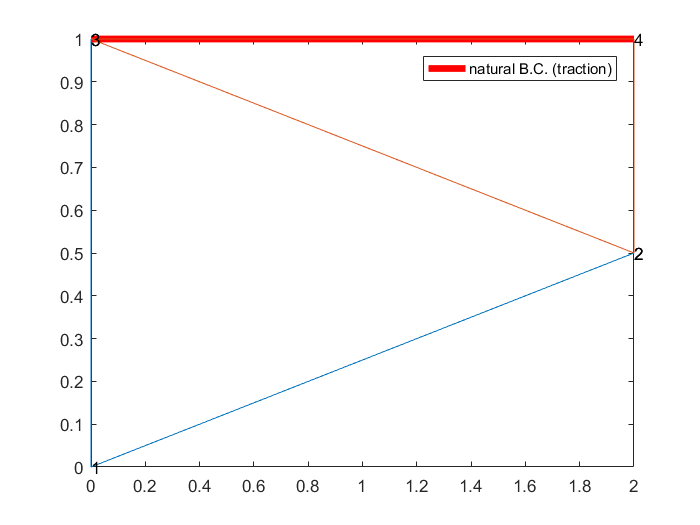
\includegraphics[width=\textwidth]{Example_3T.png}

\newpage
Answer in Matlab\\

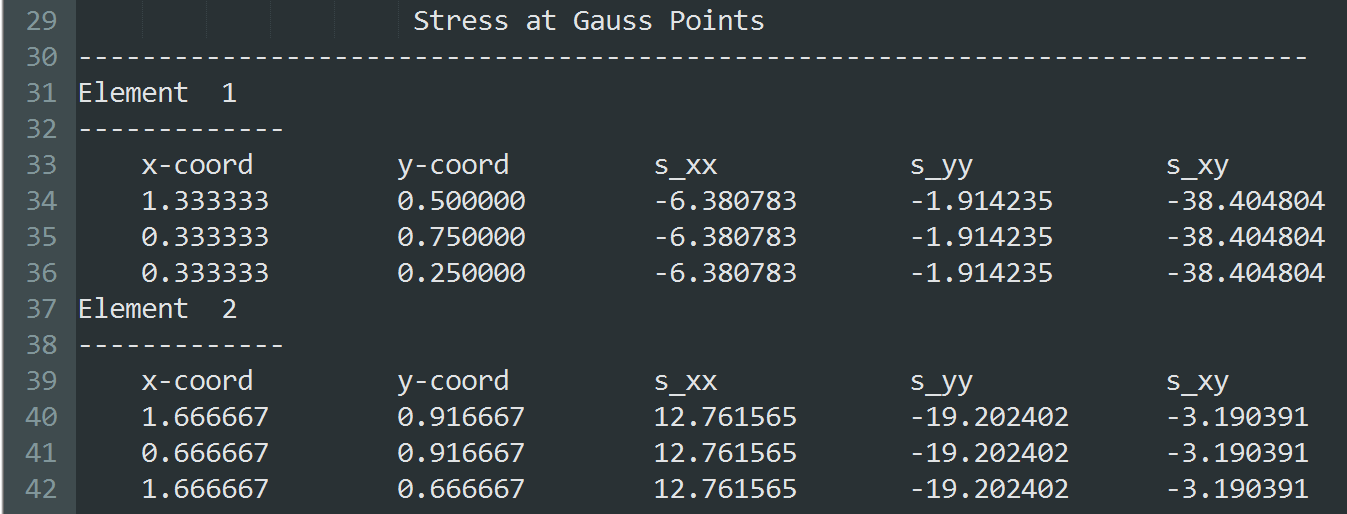
\includegraphics[width=\textwidth]{3T01.png}

Answer in Stap90\\

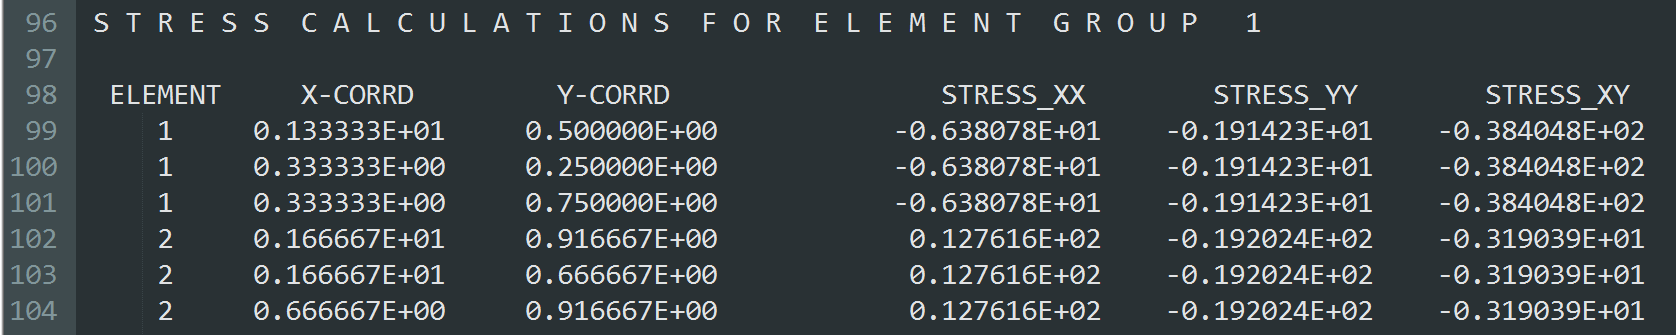
\includegraphics[width=\textwidth]{3T02.png}

\subsection{PatchTest3T}
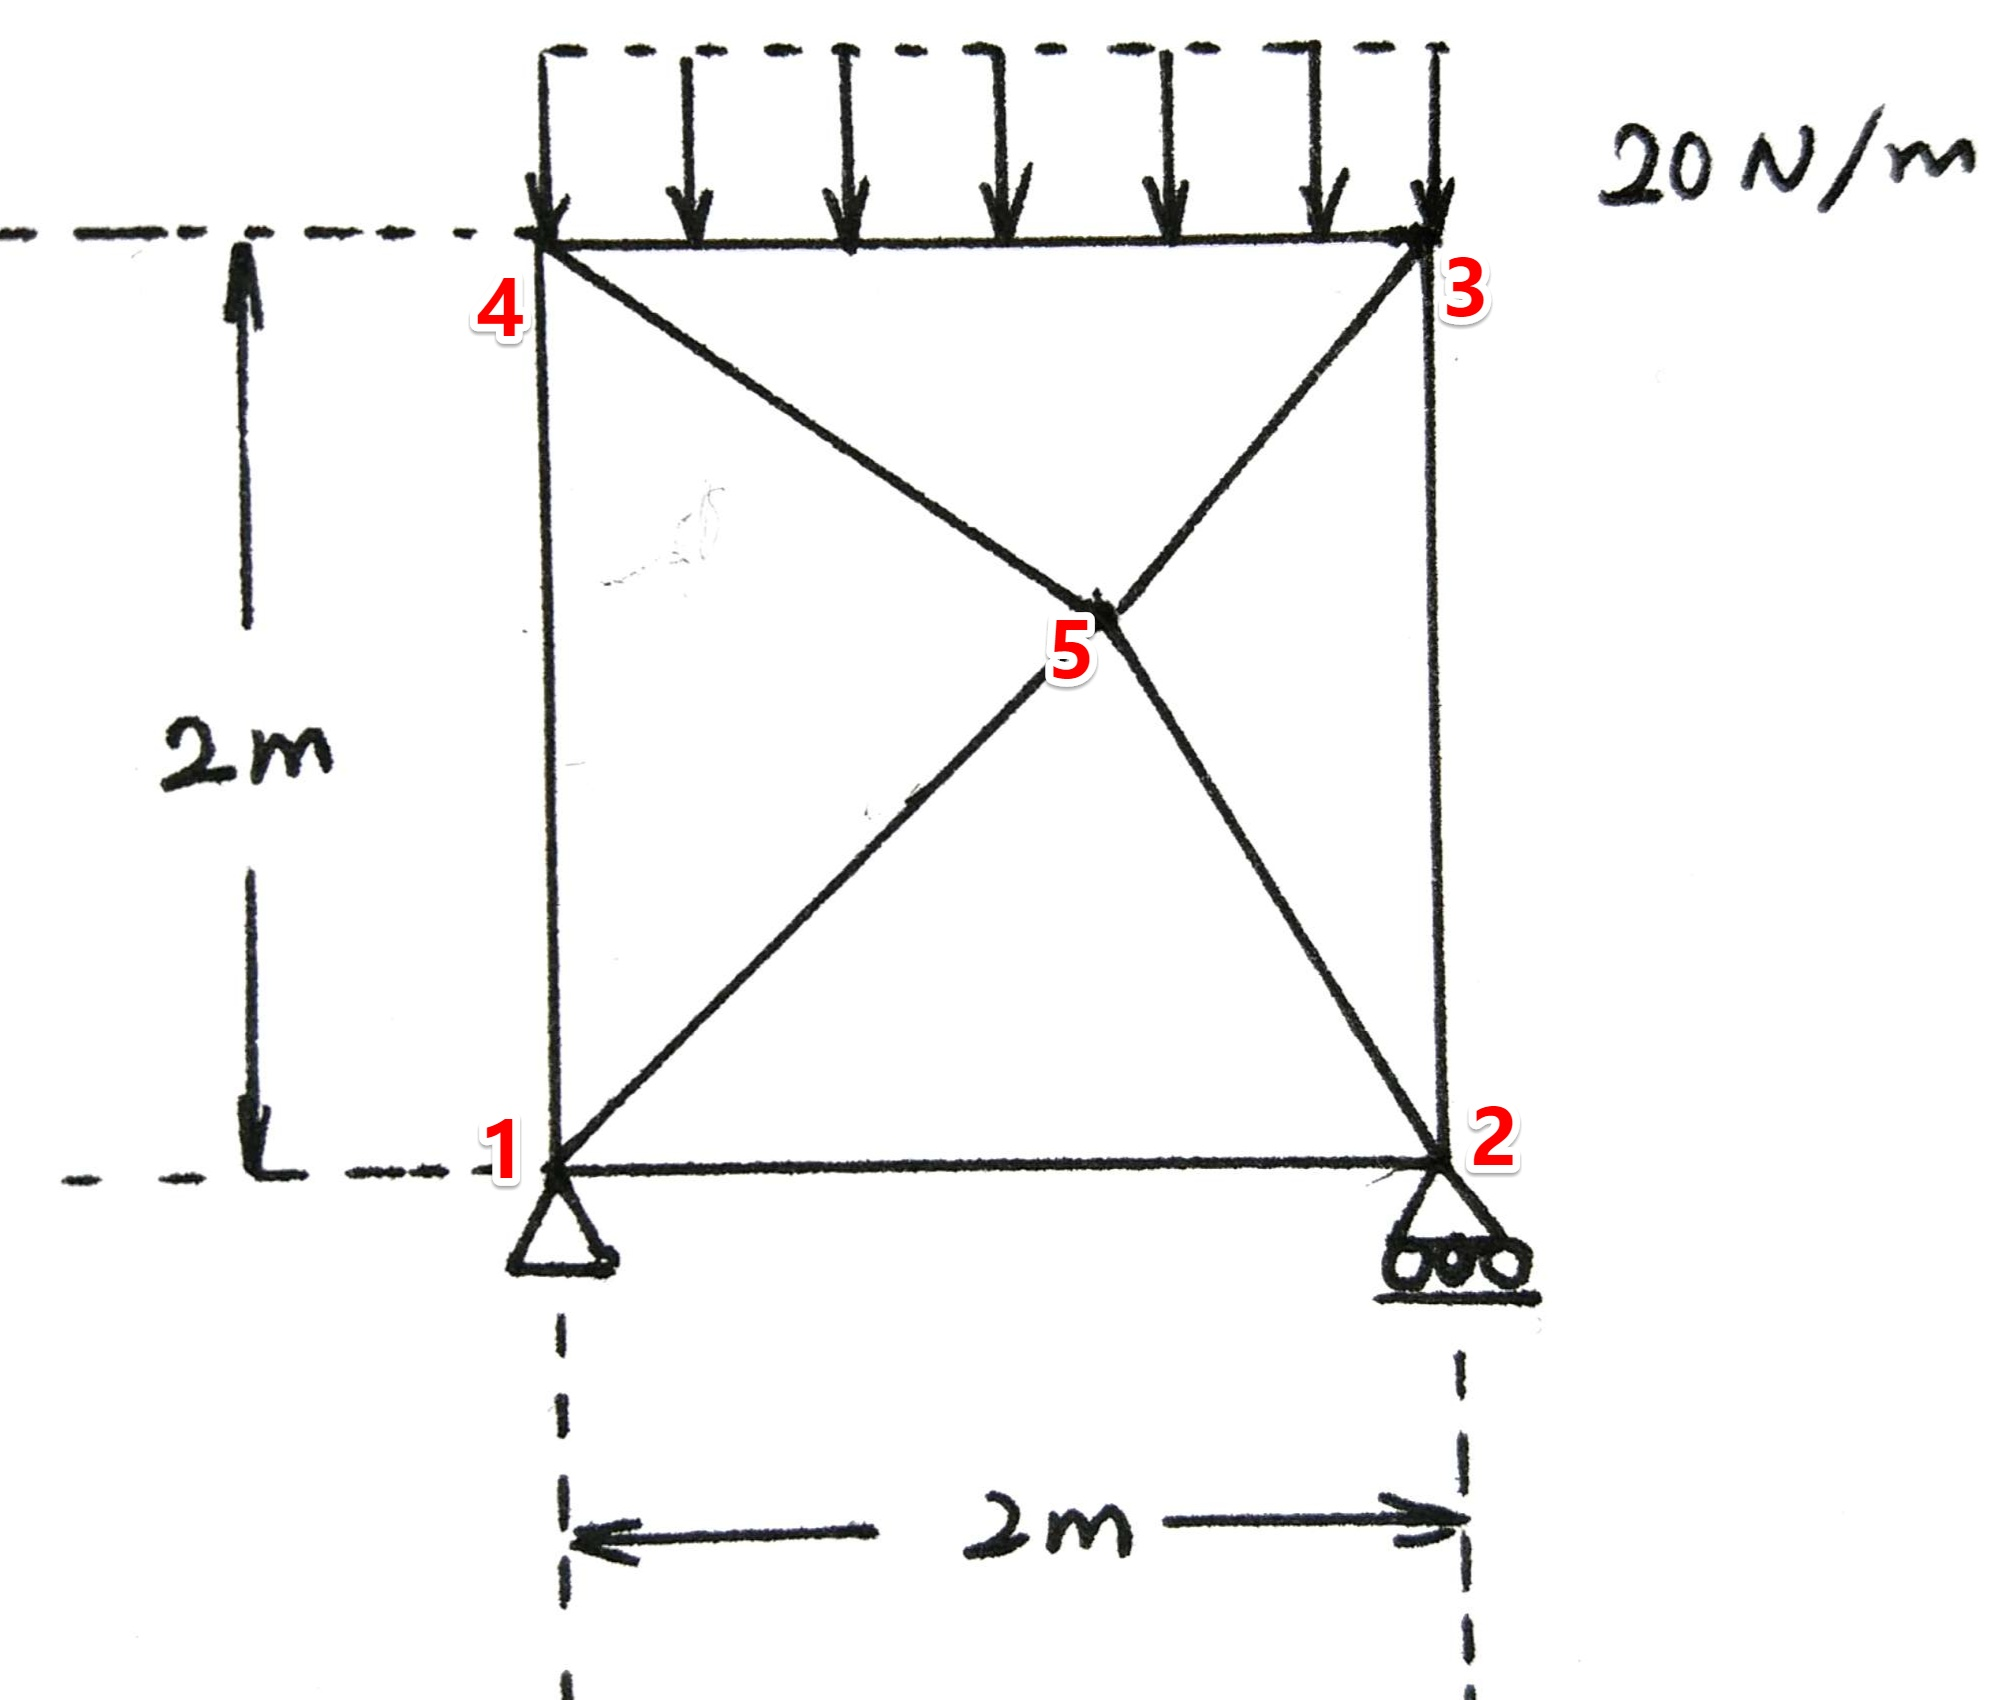
\includegraphics[width=0.8\textwidth]{PatchTest_3T.jpg}

We constrain the node 1 in xy direction and node 2 in y direction. With the pressure added on the top surface of plate, we get the constant stress that
$$s_{xx} = 0$$
$$s_{yy} = -20$$
$$s_{xy} = 0$$

Answer in Stap90\\

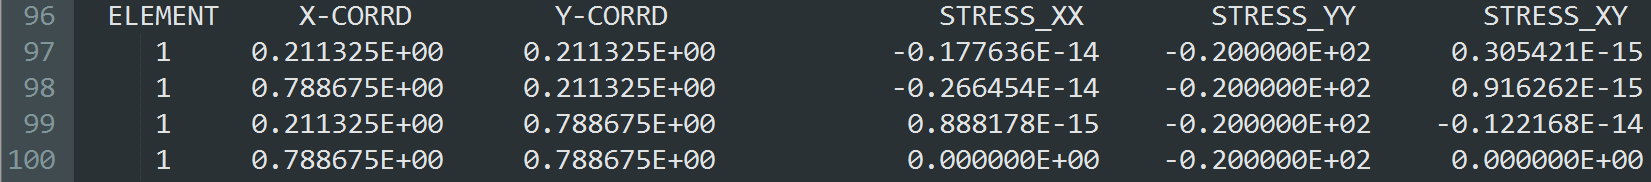
\includegraphics[width=\textwidth]{4Q03.png}

\subsection{4Q}

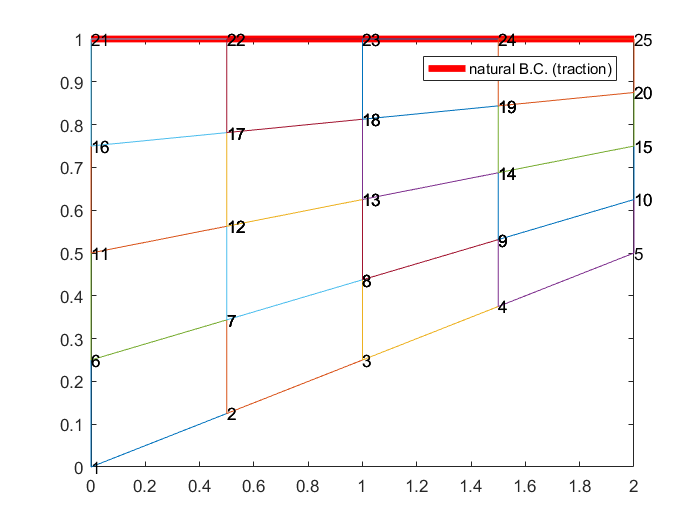
\includegraphics[width=\textwidth]{Example_4Q.png}

\newpage
Answer in Matlab

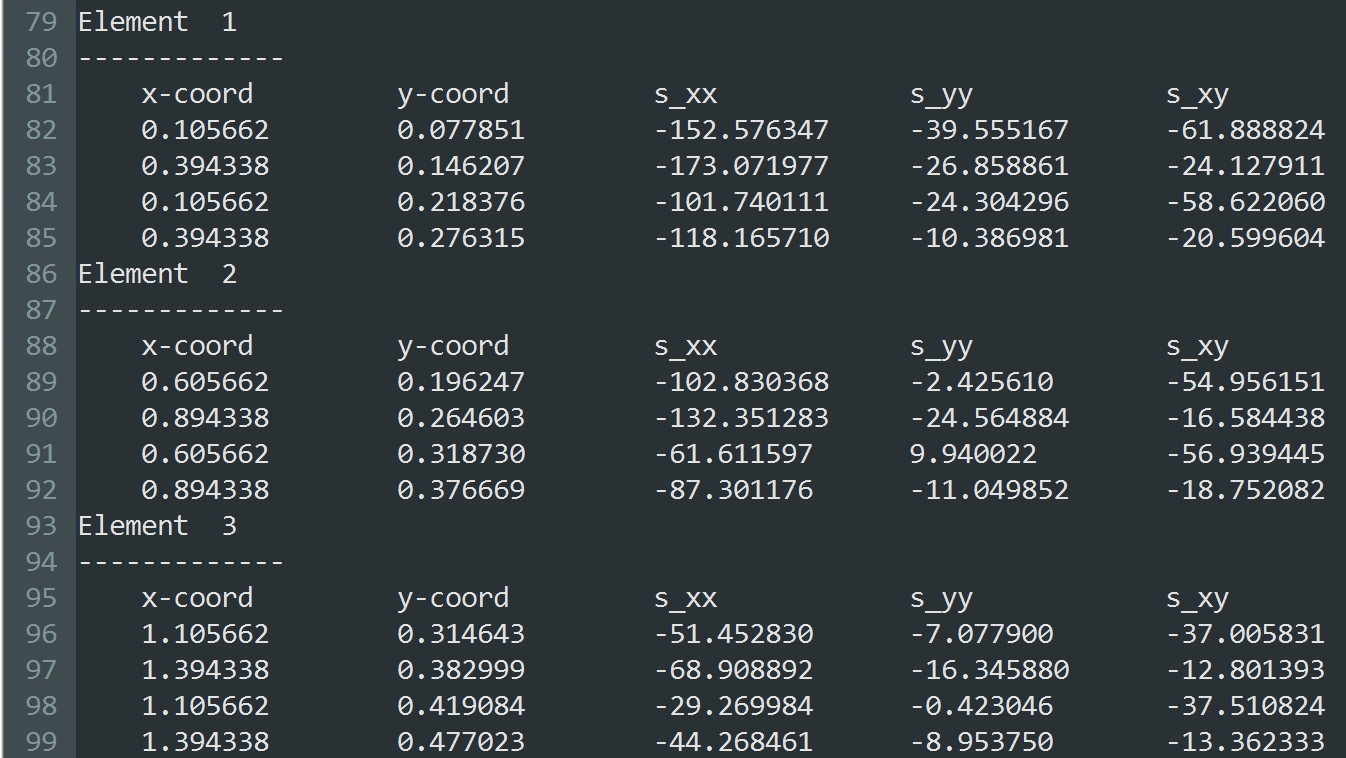
\includegraphics[width=\textwidth]{4Q01.png}

Answer in Stap90

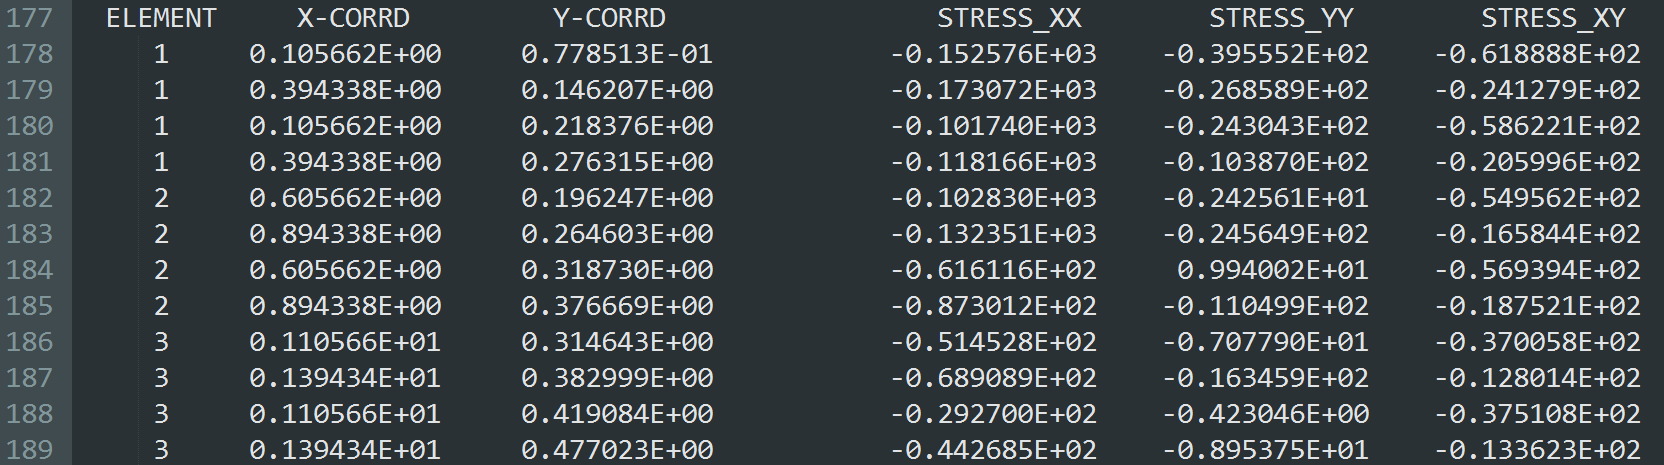
\includegraphics[width=\textwidth]{4Q02.png}

\subsection{PatchTest4Q}
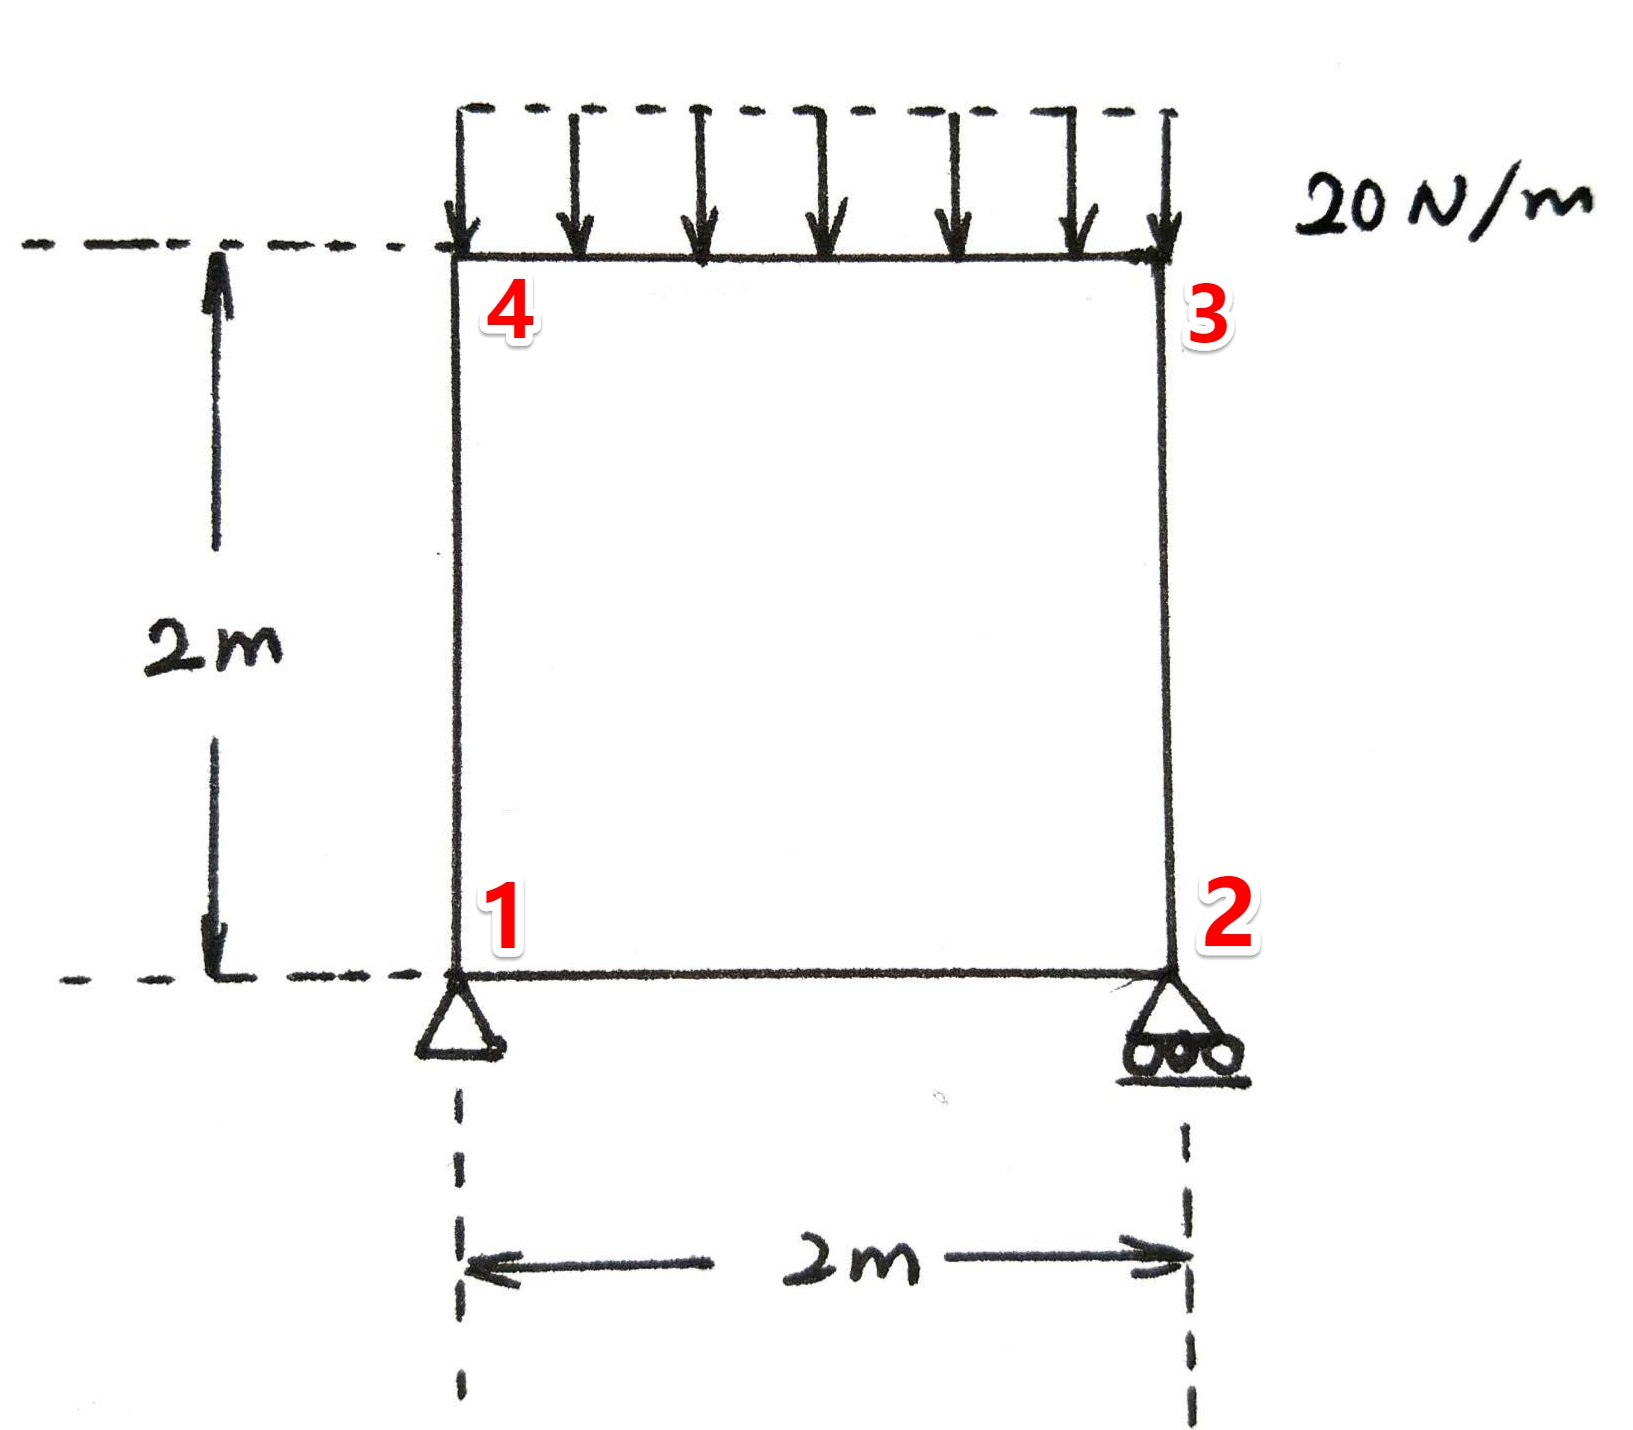
\includegraphics[width=0.8\textwidth]{Patch_4Q.jpg}

We constrain the node 1 in xy direction and node 2 in y direction. With the pressure added on the top surface of plate, we get the constant stress that
$$s_{xx} = 0$$
$$s_{yy} = -20$$
$$s_{xy} = 0$$

Answer in Stap90\\

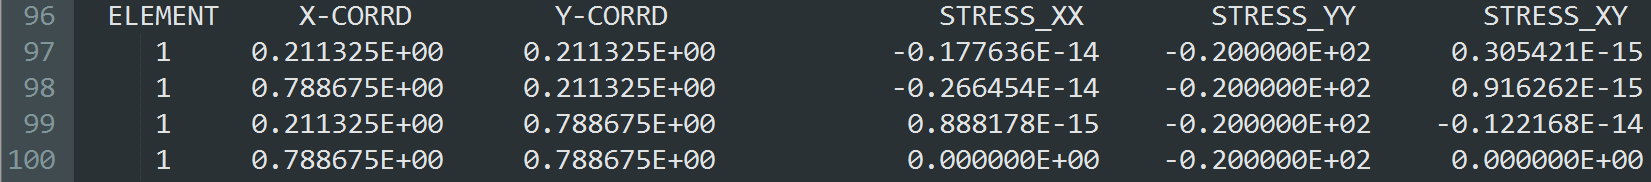
\includegraphics[width=\textwidth]{4Q03.png}

\subsection{8Q}

\subsection{9Q}

9Q的原理与4Q类似,均是用$Kd=f$进行求解,只是其组装单元刚度阵所使用的形函数不同

\begin{center}
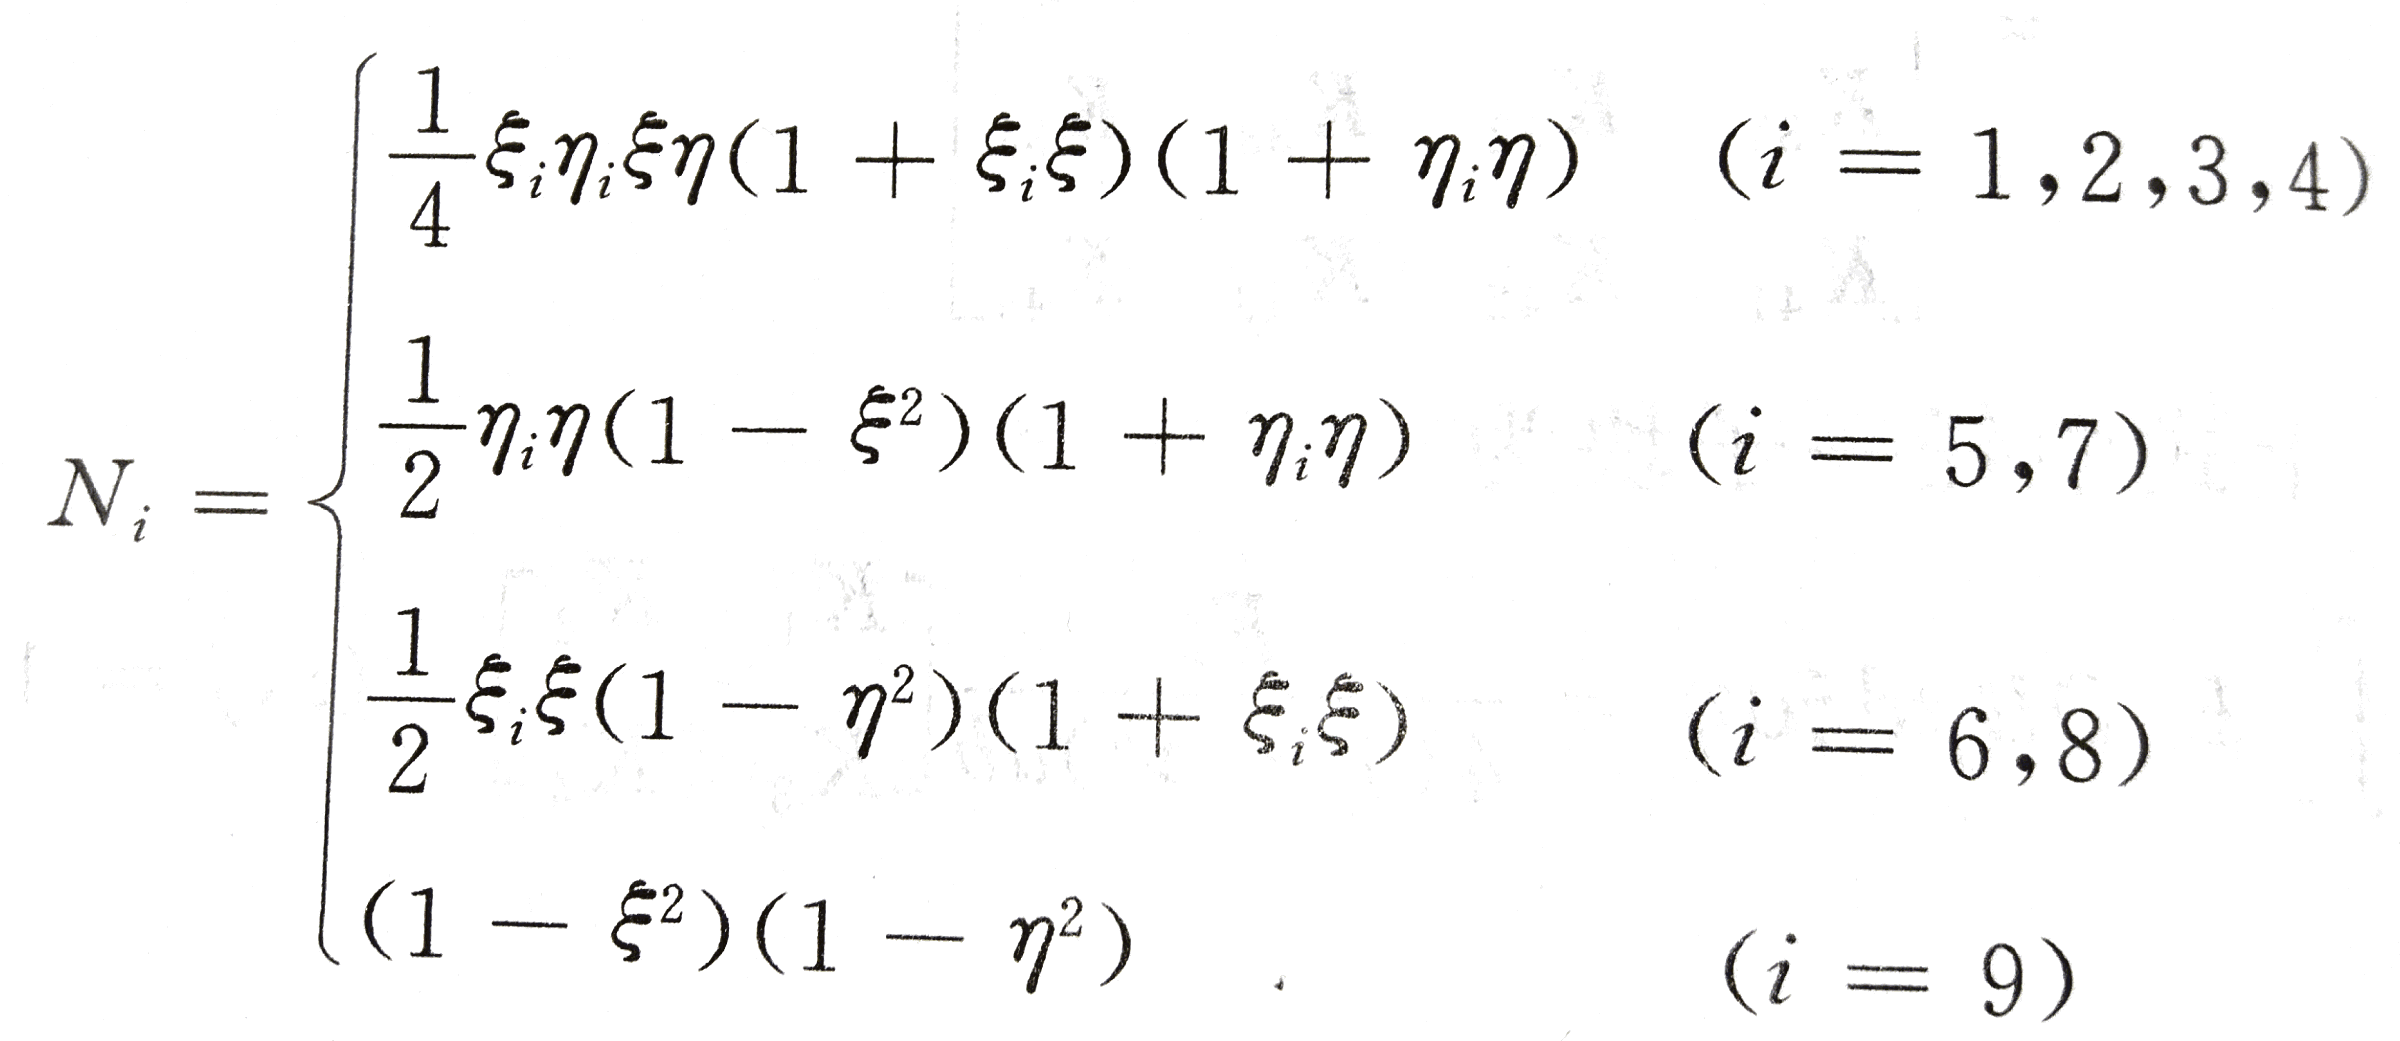
\includegraphics[width=\textwidth]{9Q01.jpg} % Include the image placeholder.png
\end{center}

PatchTest所使用的构型仍为4Q使用的Patchtest方案,即约束左下角两个自由度的位移,以及右下角Y自由度的位移,在顶部施加向下为20N/m的均布力。

其结果如下:
\begin{center}
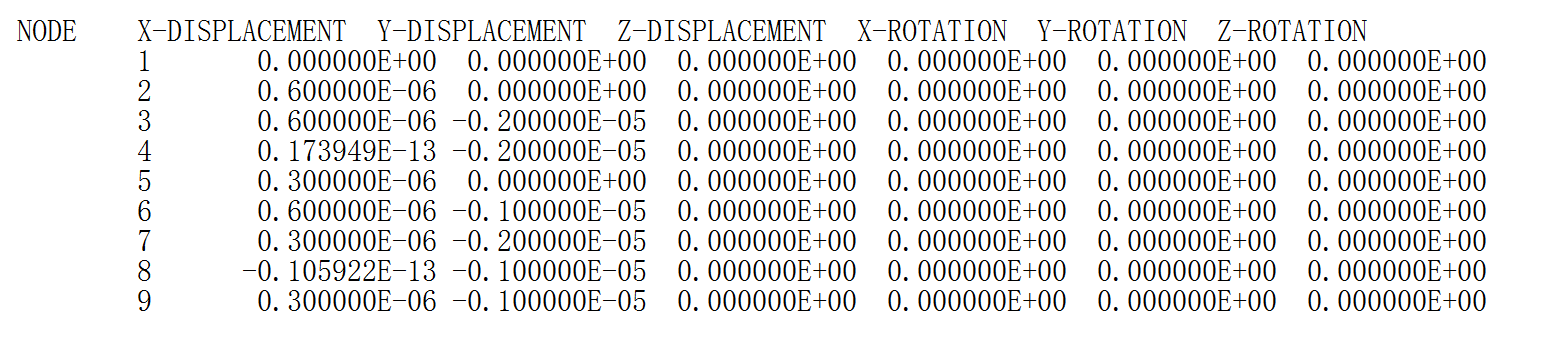
\includegraphics[width=\textwidth]{9Q02.png} % Include the image placeholder.png
\end{center}
\begin{center}
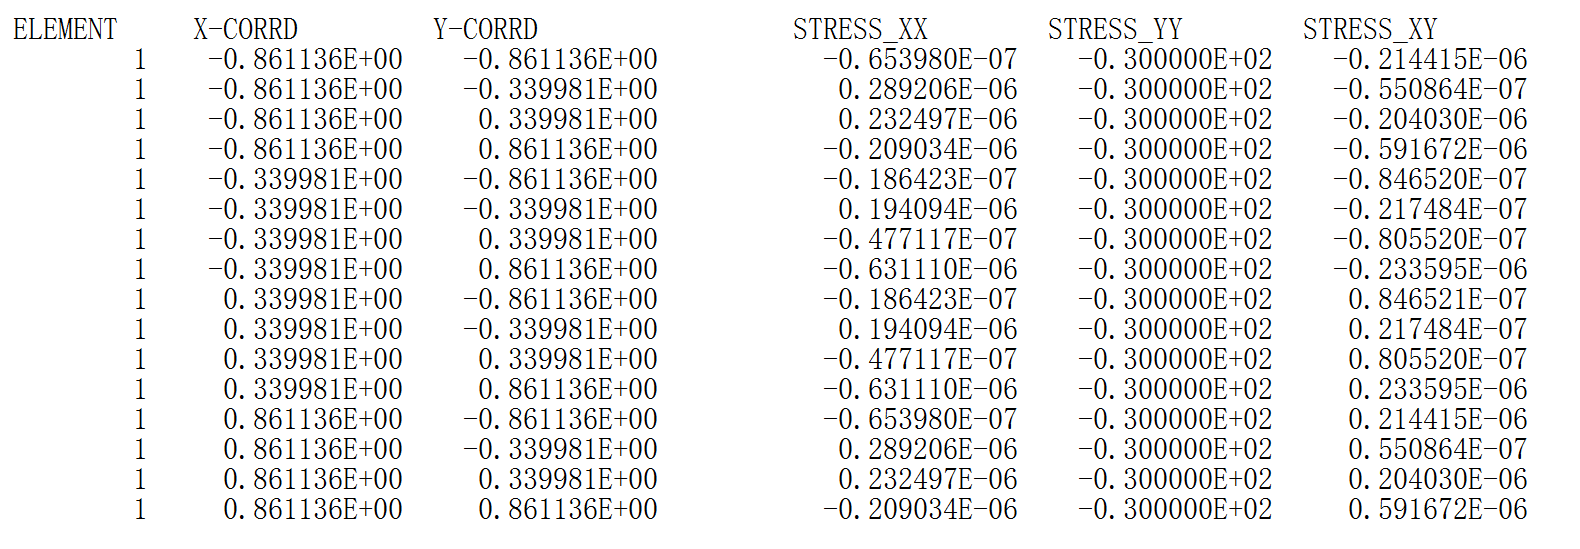
\includegraphics[width=\textwidth]{9Q03.png} % Include the image placeholder.png
\end{center}

\subsection{4T}
\paragraph{}
类似于3T单元,在三维Simplex坐标系中,可以用相对体积来作为高斯点的确定依据。指定四个节点的编号顺序为,当右手四指绕底面三顶点方向旋转时,拇指指向第四顶点方向。有:

<<<<<<< HEAD
=======
\[
N_{i}=\frac{1}{6V}(a_{i}+b_{i}x+c_{i}y+d_{i}z)
\]


作$\Lambda=\left[\begin{array}{cccc}
1 & x_{1} & y_{1} & z_{1}\\
1 & x_{2} & y_{2} & z_{2}\\
1 & x_{3} & y_{3} & z_{3}\\
1 & x_{4} & y_{4} & z_{4}
\end{array}\right]$, 有:$V=\frac{1}{6}|\Lambda|$, 且

\[
a_{1}=\left[\begin{array}{ccc}
x_{2} & y_{2} & z_{2}\\
x_{3} & y_{3} & z_{3}\\
x_{4} & y_{4} & z_{4}
\end{array}\right],\ b_{1}=-\left[\begin{array}{ccc}
1 & y_{2} & z_{2}\\
1 & y_{3} & z_{3}\\
1 & y_{4} & z_{4}
\end{array}\right],\ c_{1}=\left[\begin{array}{ccc}
1 & x_{2} & z_{2}\\
1 & x_{3} & z_{3}\\
1 & x_{4} & z_{4}
\end{array}\right],\ d_{1}=-\left[\begin{array}{ccc}
1 & x_{2} & y_{2}\\
1 & x_{3} & y_{3}\\
1 & x_{4} & y_{4}
\end{array}\right]
\]


对2,3,4其它各项按$\Lambda$行列式的代数余子式推出。

类似于8H单元,作B矩阵为$B=\nabla_{s}N$, 其每项元素均为由节点坐标决定的常数。

对单元刚度阵进行组装,最后解总刚度阵方程,思路同8H。分片测试采用立方体,分割为四个顶点对应的四面体和中心一个正四面体共5个单元,执行C类分片测试,结果通过,输入输出文件如Samples文件夹内所示。
>>>>>>> dedcc6447c9449ac1dd2040a1e7b5f4a73482371
\subsection{铁木辛柯梁}
\subsubsection{基本原理}
与欧拉梁不同的是,铁木辛柯梁在转角和挠度上同时插值,这样就考虑了剪切的影响。
铁木辛柯梁的刚度矩阵分为剪切部分和弯曲部分,为了避免剪切锁闭,剪切部分采用减缩积分。
在一次插值的情况下,剪切部分采用1点高斯积分。
铁木辛柯梁的难点还是三维情况下刚度阵的组装,这里包含了材料力学意义下的扭转,铁木辛柯梁意义下的弯曲,和普通的简单拉伸。我们把这些刚度元素组装到合适的位置。
铁木辛柯梁的刚度阵如下图。其中剪切部分有一个截面修正因子,这里和课上讲的修整因子成倒数关系。
取
$$k=\frac{10(1+\nu)}{12+11\nu}$$
\begin{center}
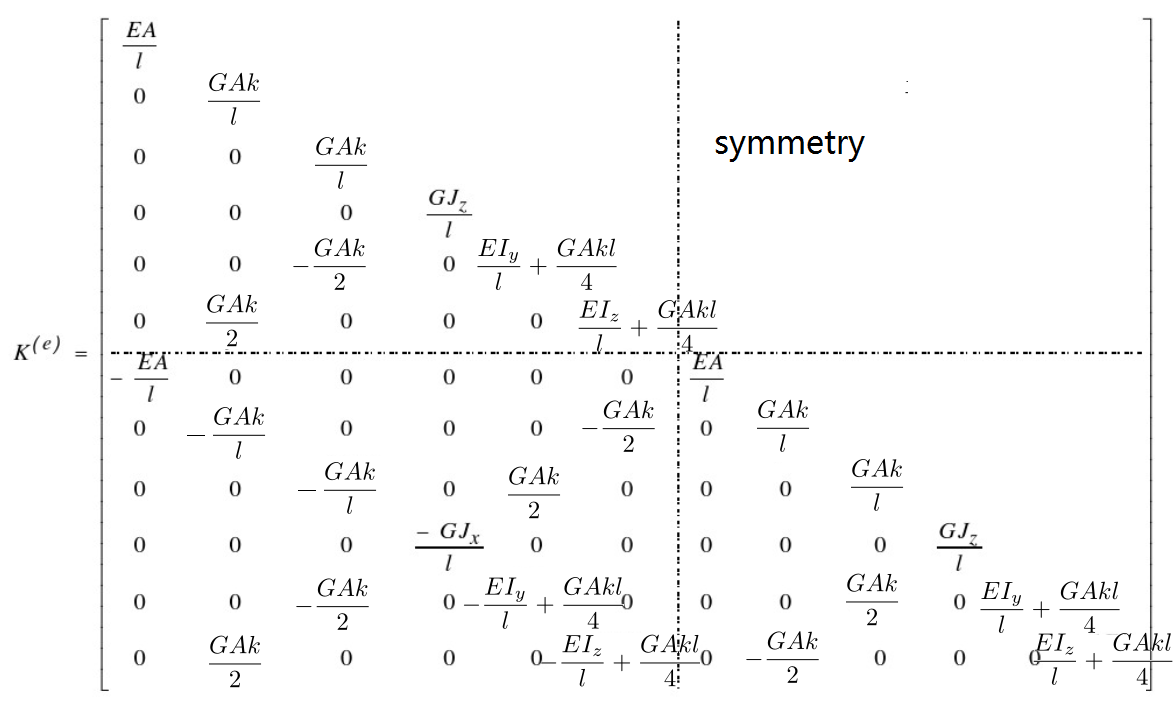
\includegraphics[width=1.0\textwidth]{timoshenko1.png}
\end{center}
载荷以及右端力向量如图。
\begin{center}
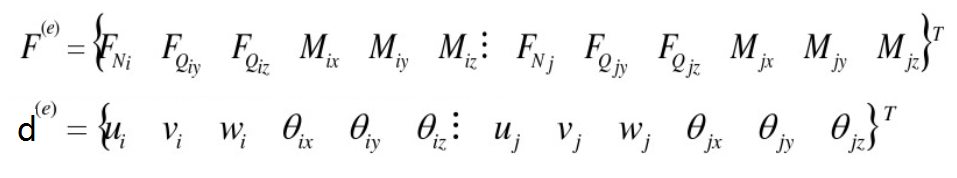
\includegraphics[width=1.0\textwidth]{beam2.png}
\end{center}
\subsubsection{输入输出}
\paragraph{}For controlling messages of nodals:
\begin{center}
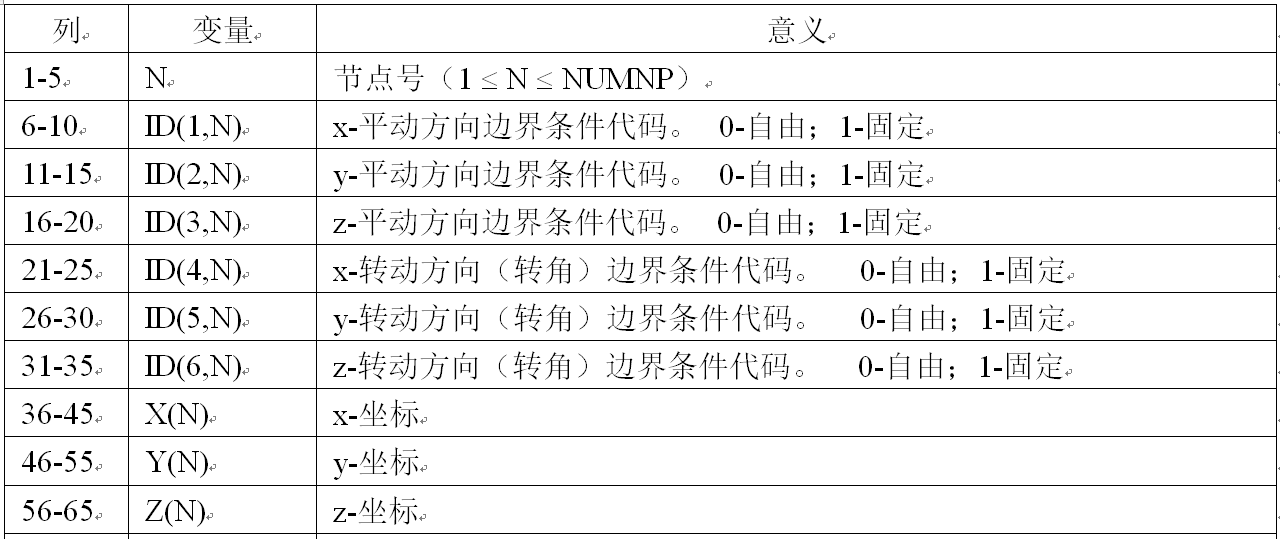
\includegraphics[width=1.0\textwidth]{beam3.png}
\end{center}
\paragraph{}For information about the loads:
\begin{center}
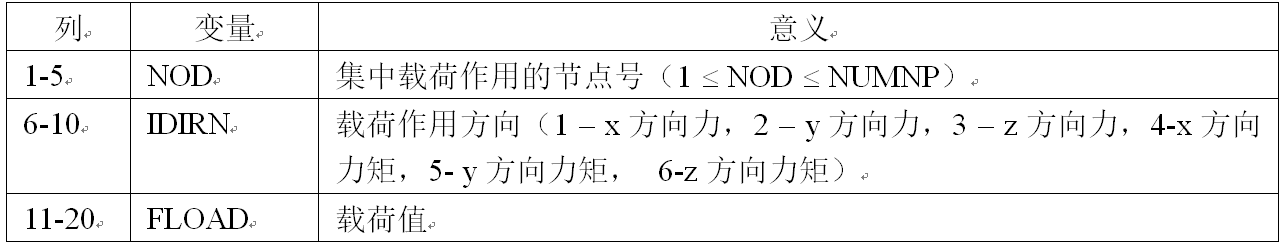
\includegraphics[width=1.0\textwidth]{beam4.png}
\end{center}
\paragraph{}For information about the materials:
\begin{center}
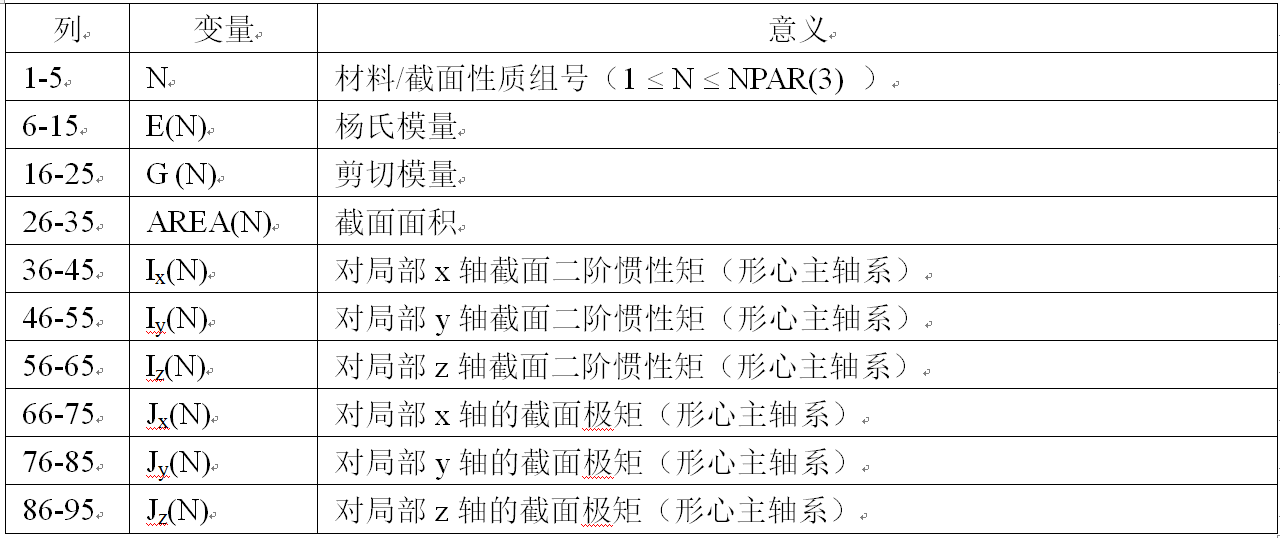
\includegraphics[width=1.0\textwidth]{beam5.png}
\end{center}
\paragraph{}For information about the element connectivity:
\begin{center}
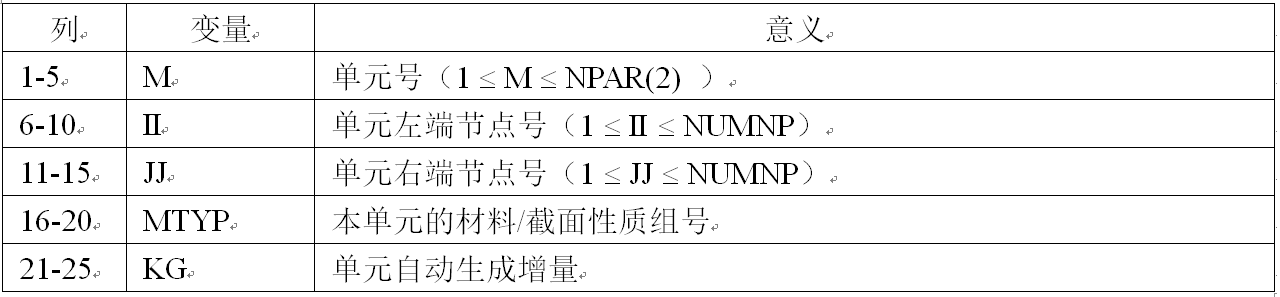
\includegraphics[width=1.0\textwidth]{beam6.png}
\end{center}
\subsubsection{分片试验结果收敛性分析}
需要注意的是,铁木辛柯梁对一般截面并没有精确解,但是对于圆截面还是可以分析收敛性。误差的能量范数是一阶收敛的。并且减缩积分能获得更精确的结果。
最重要的是,通过铁木辛柯梁,我对有限元中减缩积分的方法有了新的理解。
铁木辛柯梁只是一种梁模型,通过铁木辛柯梁和欧拉梁的编写,我发现只要给定一种弯曲模型,就可以很轻松地算出这种模型的有限元刚度阵,进而进行计算。
\begin{center}
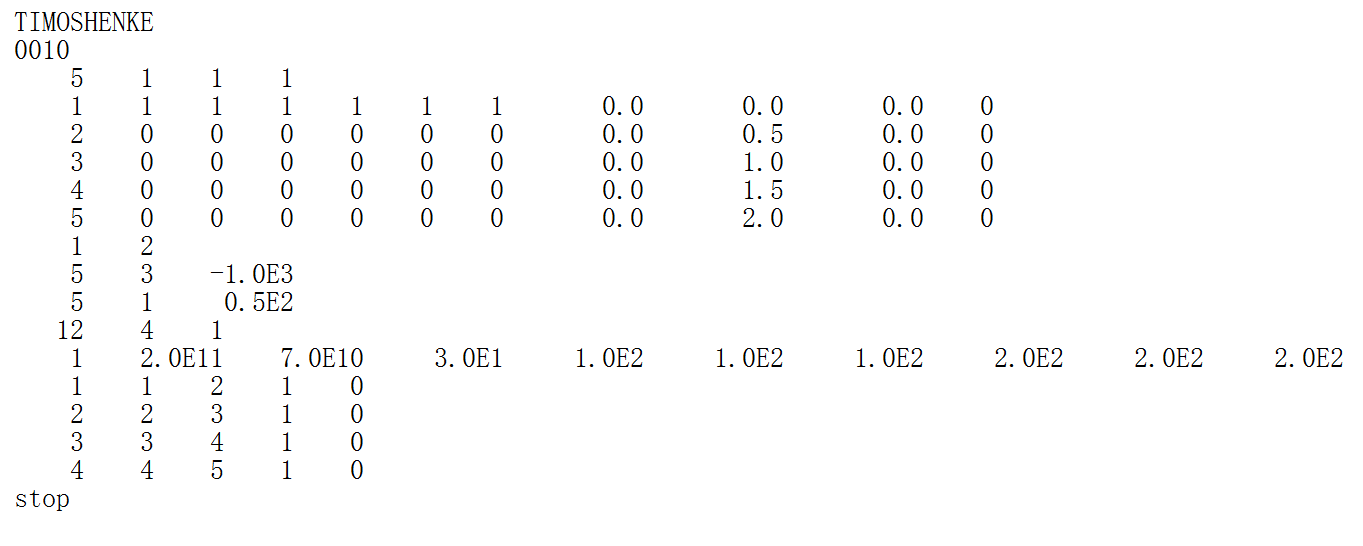
\includegraphics[width=1.0\textwidth]{timoshenko2.png}
\end{center}
\begin{center}
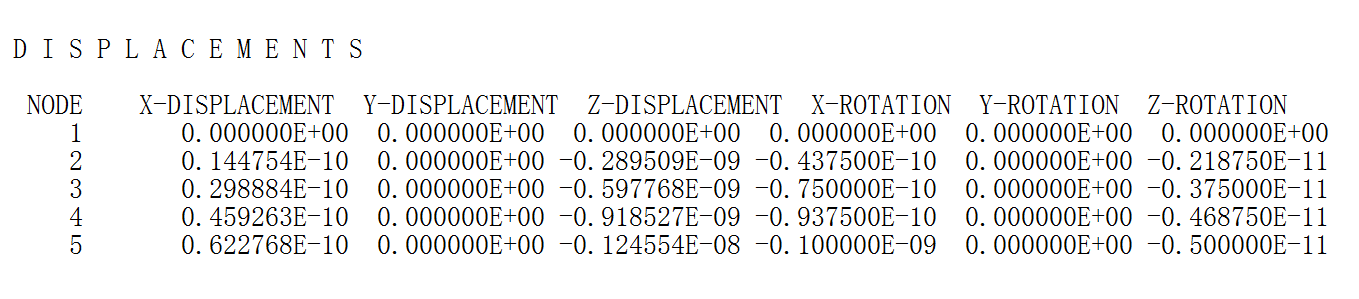
\includegraphics[width=1.0\textwidth]{timoshenko3.png}
\end{center}
\subsection{Plate}

    \subsection{Formula Derivation}
    In the stap90, I create two kinds of plate elements, both of which are for thick plate.

    The difference between them is the number of the nodes in each element. The first type has only 4 nodes
    each element, the same as 4Q, while the other has 8. I would explain the reason below.
    \subsubsection{Plate4Q}
    
     The Plate4Q element is almost the same as 4Q. We use isoparametric element by represent both
     the transformation of coordination and the w, $\beta_x$, $\beta_y$ with the same bunch of bilinear
     shape function.

     The only disparity is the formula of strain and stress, as shown below.
     
     As for strain:
     \begin{equation}
     \left( \begin{array} {c}
        \epsilon_{xx} \\
        \epsilon_{yy} \\
        \gamma_xy \end{array}\right) = -z
     \left( \begin{array} {c}
        \frac{\partial \beta_x}{\partial x} \\
        \frac{\partial \beta_y}{\partial y} \\
        \frac{\partial \beta_x}{\partial y}+\frac{\partial \beta_y}{\partial x} \end{array}\right)
     \end{equation}
          \begin{equation}
     \left( \begin{array} {c}
        \gamma_{xz} \\
        \gamma_{yz} \end{array}\right) =
     \left( \begin{array} {c}
        \frac{\partial w}{\partial x} - \gamma_x\\
        \frac{\partial \beta_y}{\partial y} - \gamma_y \end{array}\right)
     \end{equation}
     
     And for stress:
     \begin{equation}
     \left( \begin{array} {c}
        \tau_{xx} \\
        \tau_{yy} \\
        \tau_xy \end{array}\right) = -z \frac{E}{1-\nu^2}
     \left( \begin{array} {ccc}
        1 & \nu & 0 \\
        \nu & 1 & 0\\
        0 & 0 & \frac{1-\nu}{2} \end{array}\right)
     \left( \begin{array} {c}
        \epsilon_{xx} \\
        \epsilon_{yy} \\
        \gamma_xy \end{array}\right)
     \end{equation}
     \begin{equation}
     \left( \begin{array} {c}
        \tau_{xz} \\
        \tau_{yz} \end{array}\right) = \frac{E}{2(1+\nu)}
     \left( \begin{array} {c}
        \gamma_{xz} \\
        \gamma_{yz} \end{array}\right)
     \end{equation}
     
     The last thing we need is the formula for total energy:
     \begin{equation}
     \begin{split}
        \Pi = &\frac{1}{2}\int_A\int^{h/2}_{-h/2}
        \left( \begin{array} {ccc}
        \epsilon_{xx} & \epsilon_{yy} & \gamma_xy \end{array}\right)
             \left( \begin{array} {c}
        \tau_{xx} \\
        \tau_{yy} \\
        \tau_xy \end{array}\right)dzdA \\ &+ 
        \frac{k}{2}\int_A\int^{h/2}_{-h/2}
                \left( \begin{array} {cc}
        \epsilon_{xz} & \epsilon_{yz}\end{array}\right)
        \left( \begin{array} {c}
        \tau_{xz} \\
        \tau_{yz} \end{array}\right)dzdA
     \end{split}
     \end{equation}
     Then we could use the variational principle to gain the specific formula of each term in the equation below.
     \begin{equation}
        (K_\kappa + K_\gamma)d = f
     \end{equation}
     However, I soon find out that this element could not pass any kinds of patch test, since it has represent bending. Therefore, I choose to modify the element to 8 nodes.
     \subsubsection{Plate8Q}
     The increase of the number of nodes barely change anything. The only alternation is using the serendipity shape function for 8 nodes instead of the bilinear one of 4 nodes.
     \subsection{Convergence Analysis}
     The convergence of the two elements are the same as 4Q and 8Q. 
     
     Both could exactly reconstruct linear field. And the plate8Q element could only reconstruct a quadratic field only is the coordination transformation is linear. 
     \subsection{Patch Test}
     After discussion, our group decides to use a simple quadratic w field to do the patch test.
     
     As we have no idea the deformation formula for a plate, we simplified it to a beam by restricting the $\beta_y$ for every node and fixed one end of the board to make it a cantilever.
     
     From the formula of a cantilever in the situation that only a torque acts on the free end.
     \begin{equation}
        \begin{split}
            w &= \frac{Mx^2}{2EI} \\
            \beta_x &= \frac{Mx}{EI} \\
        \end{split}
     \end{equation}
     In the patch test, we set the length of the board as 40m, the width as 2m, and the thickness as 0.1m, E as $10^10$, $\nu$ as 0, and the total M in one end as 80 N.M.
     
     Therefore, 
     \begin{equation}
        I = 2\times\int^{0.05}_{-0.05} z^2dz = \frac{1}{6000}
     \end{equation}
     Put those numbers back to (7), we have,
     \begin{equation}
        \begin{split}
            w &= 2.4\times10^{-5} x^2 \\
            \beta_x &= 4.8\times10^{-5} x \\
        \end{split}     
     \end{equation}
     And the result from the two kinds of elements are:
     
     The 4 nodes element:
        \begin{center}
            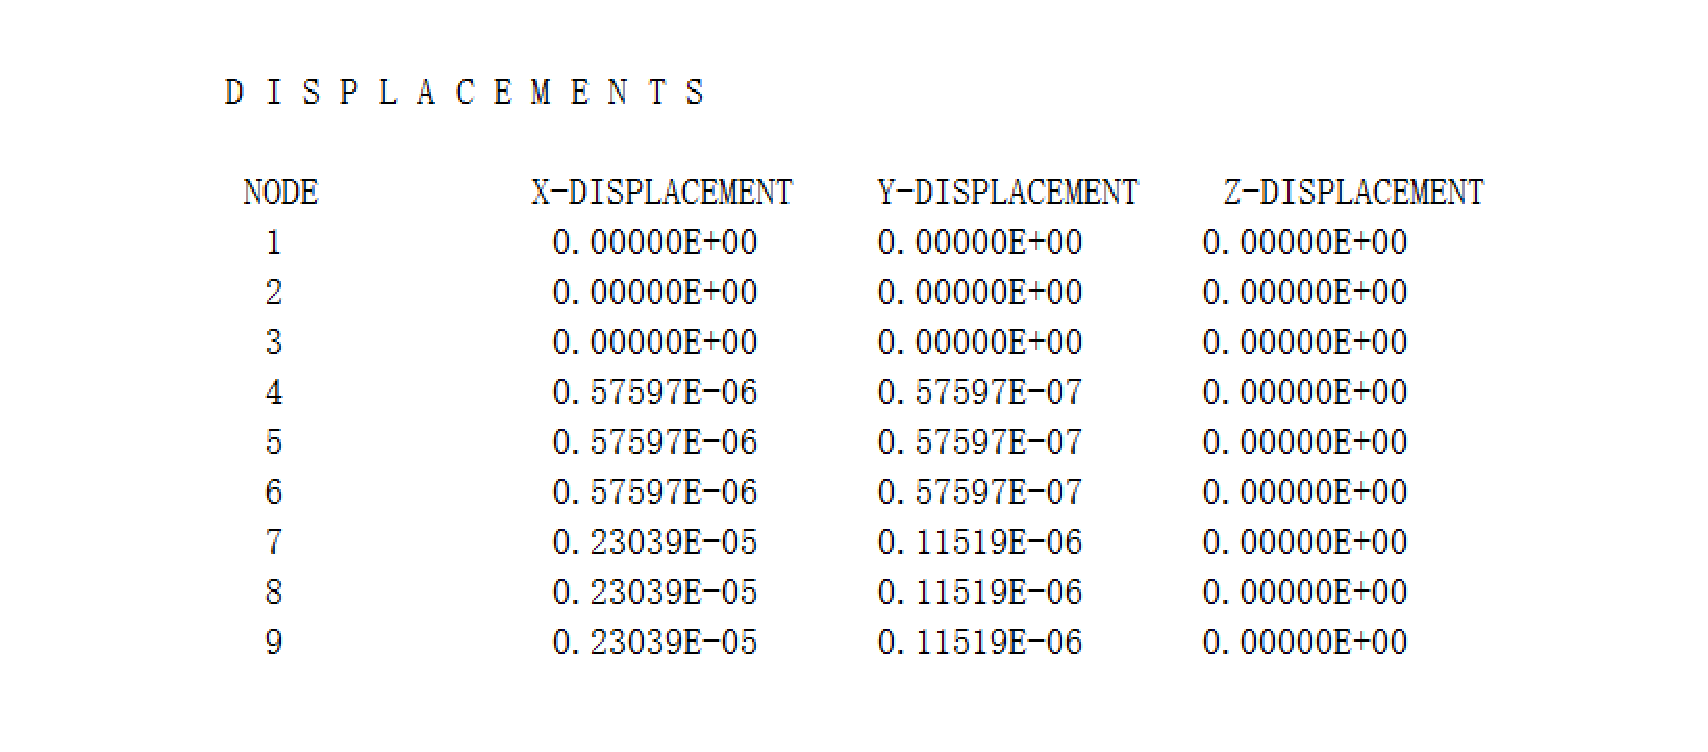
\includegraphics[width=12.30cm,height=5.41cm]{plate4Q.pdf}
        \end{center}
    
    The 8 nodes elements:
        \begin{center}
            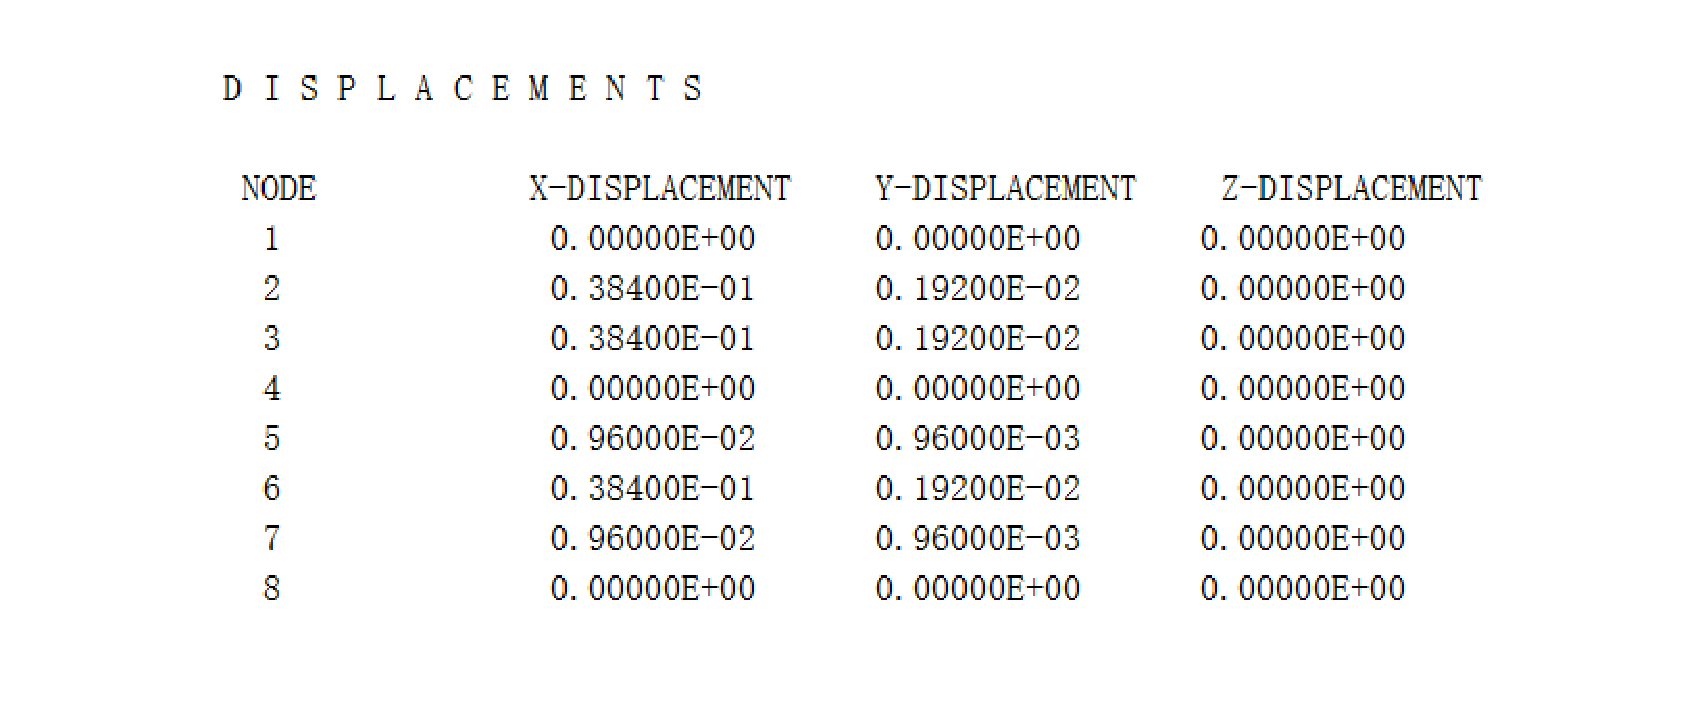
\includegraphics[width=12.15cm,height=5.13cm]{plate8Q.pdf}
        \end{center}
    The nodes are indexed in the following way.
        \begin{center}
            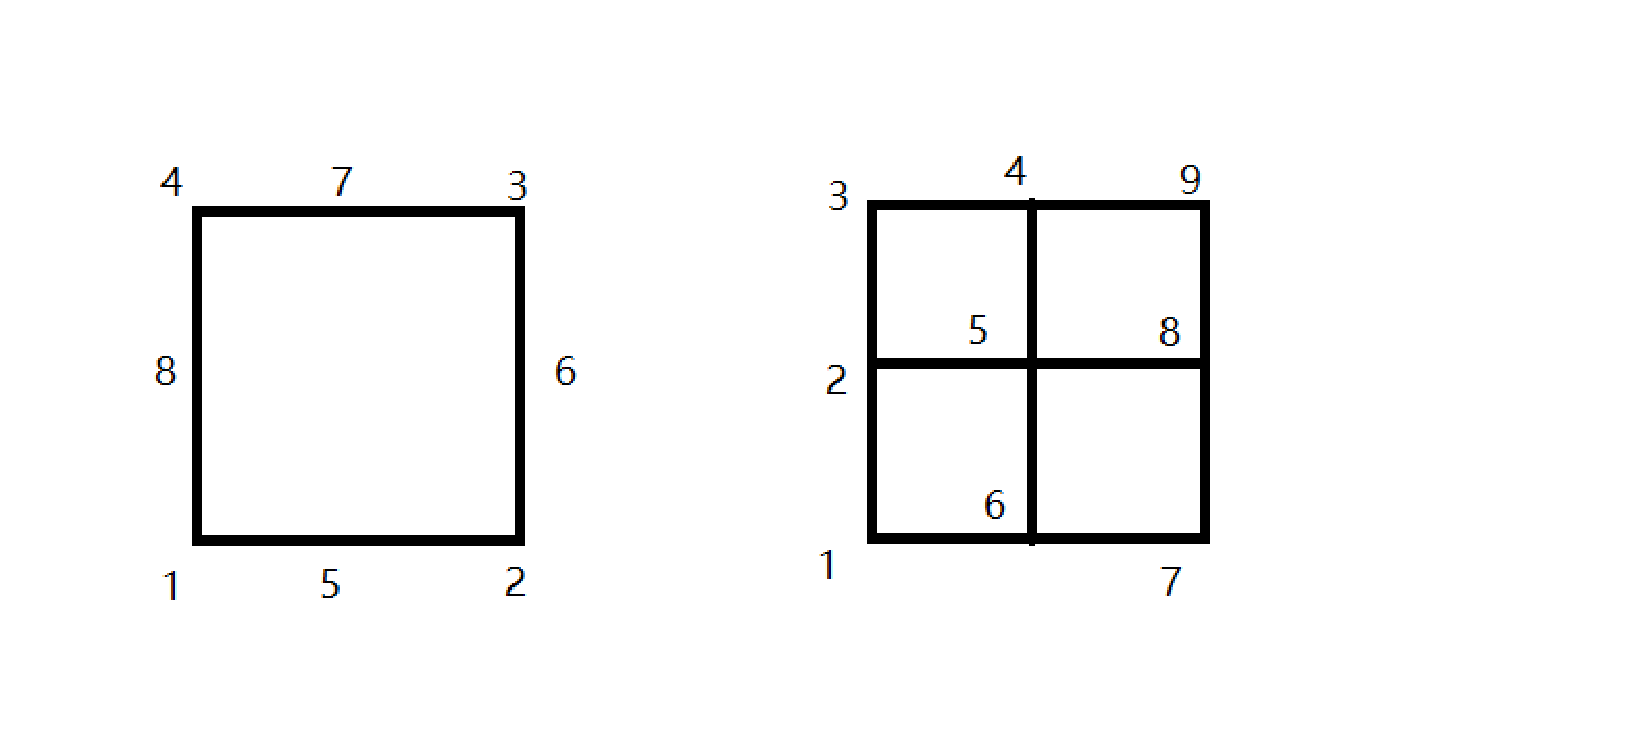
\includegraphics[width=7.84cm,height=3.60cm]{index.pdf}
       \end{center}
    As we could see, since the 4 nodes element could not represent bending, the result of it was poor, while the 8 nodes element successfully passed the patch test. 
    \subsection{Application}
    I use the Abaqus to check the 2 element.
    
    The problem is that two concentrate force act on the corner of a square board.
        \begin{center}
            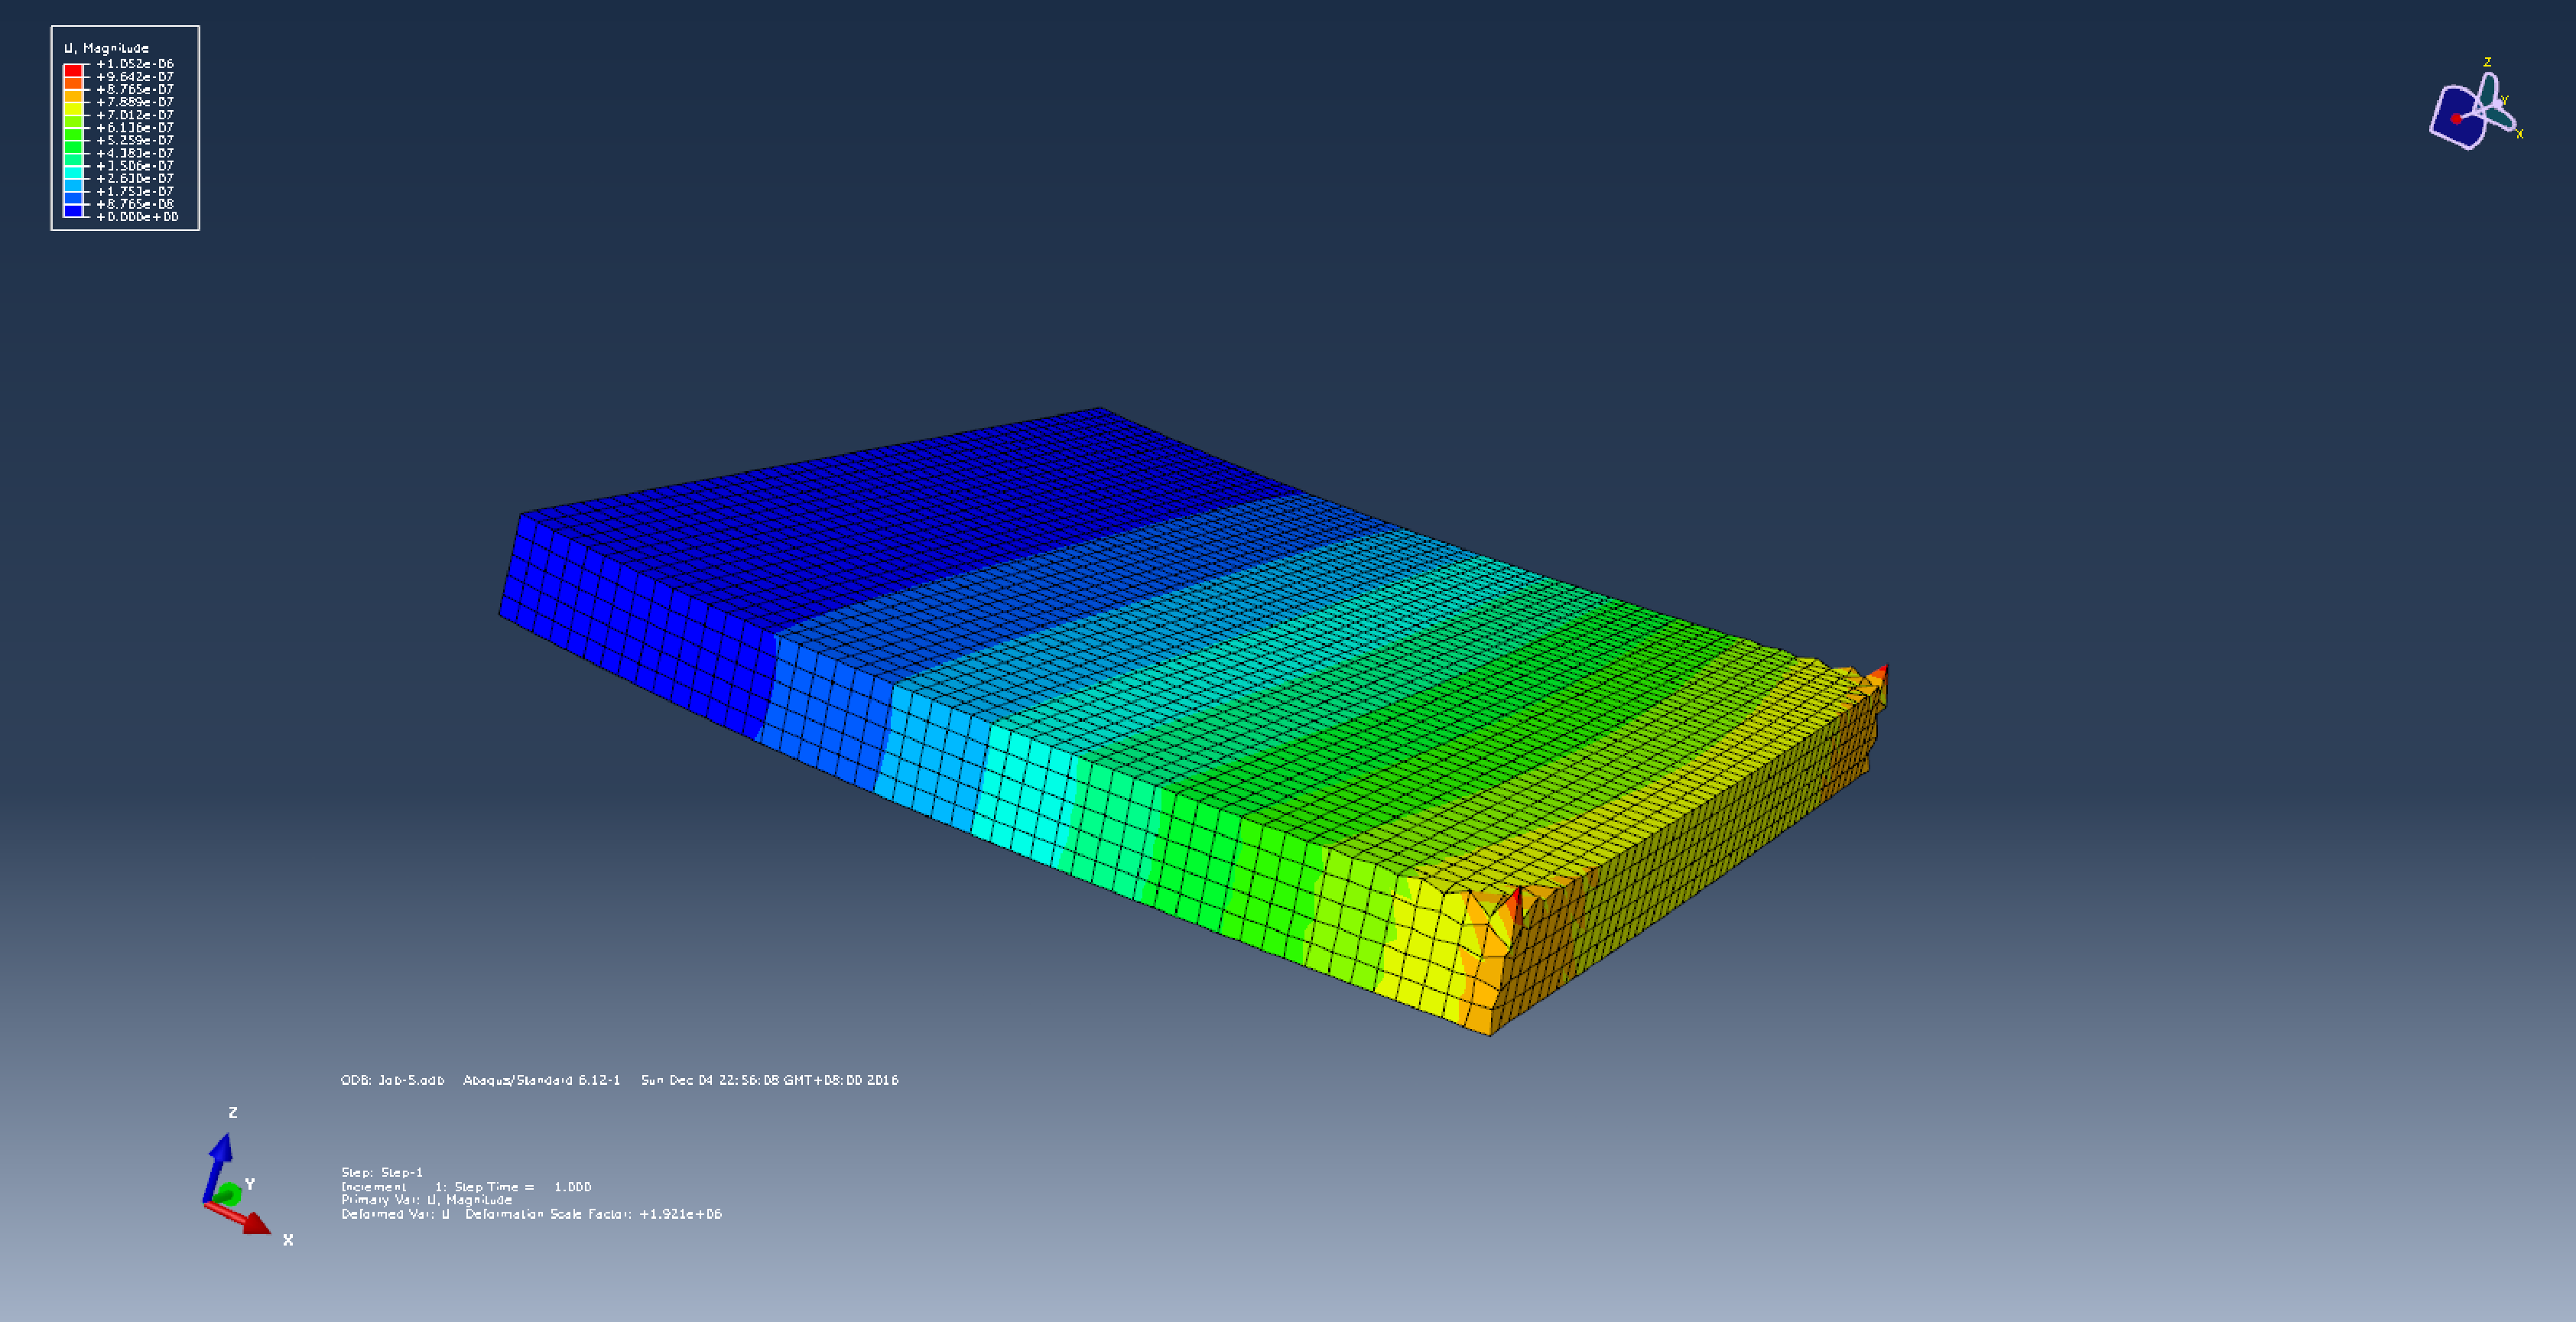
\includegraphics[width=12cm,height=6cm]{abaqus.pdf}
        \end{center}
    The maxima of displacement is 1.05E-6
    
    In the plate4Q element, I use 16 elements. The answer is shown below.
        \begin{center}
            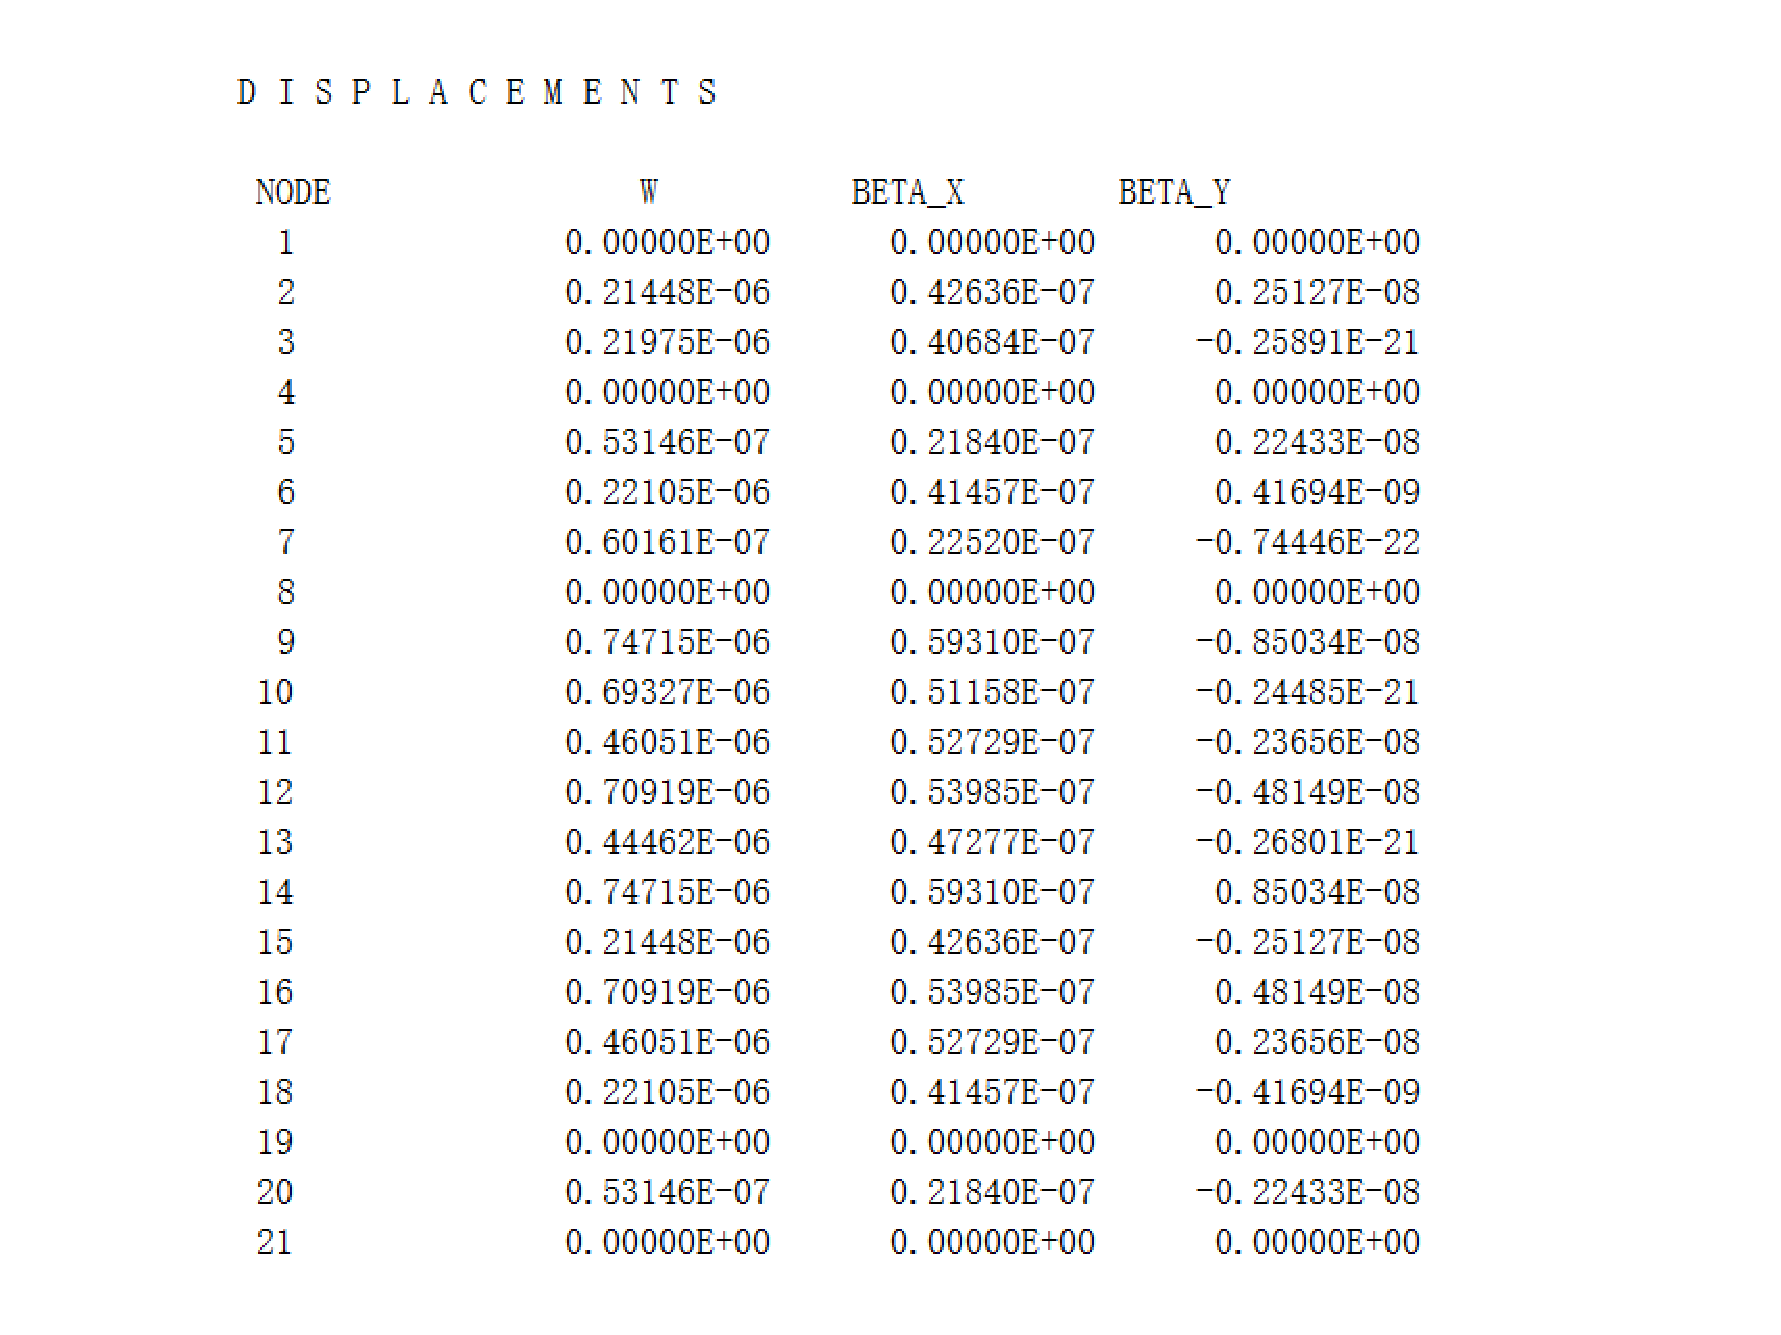
\includegraphics[width=8.55cm,height=6.41cm]{plate8Q_appl.pdf}
        \end{center}
    In the plate8Q element, I use 4 elements. The answer is shown below.
        \begin{center}
            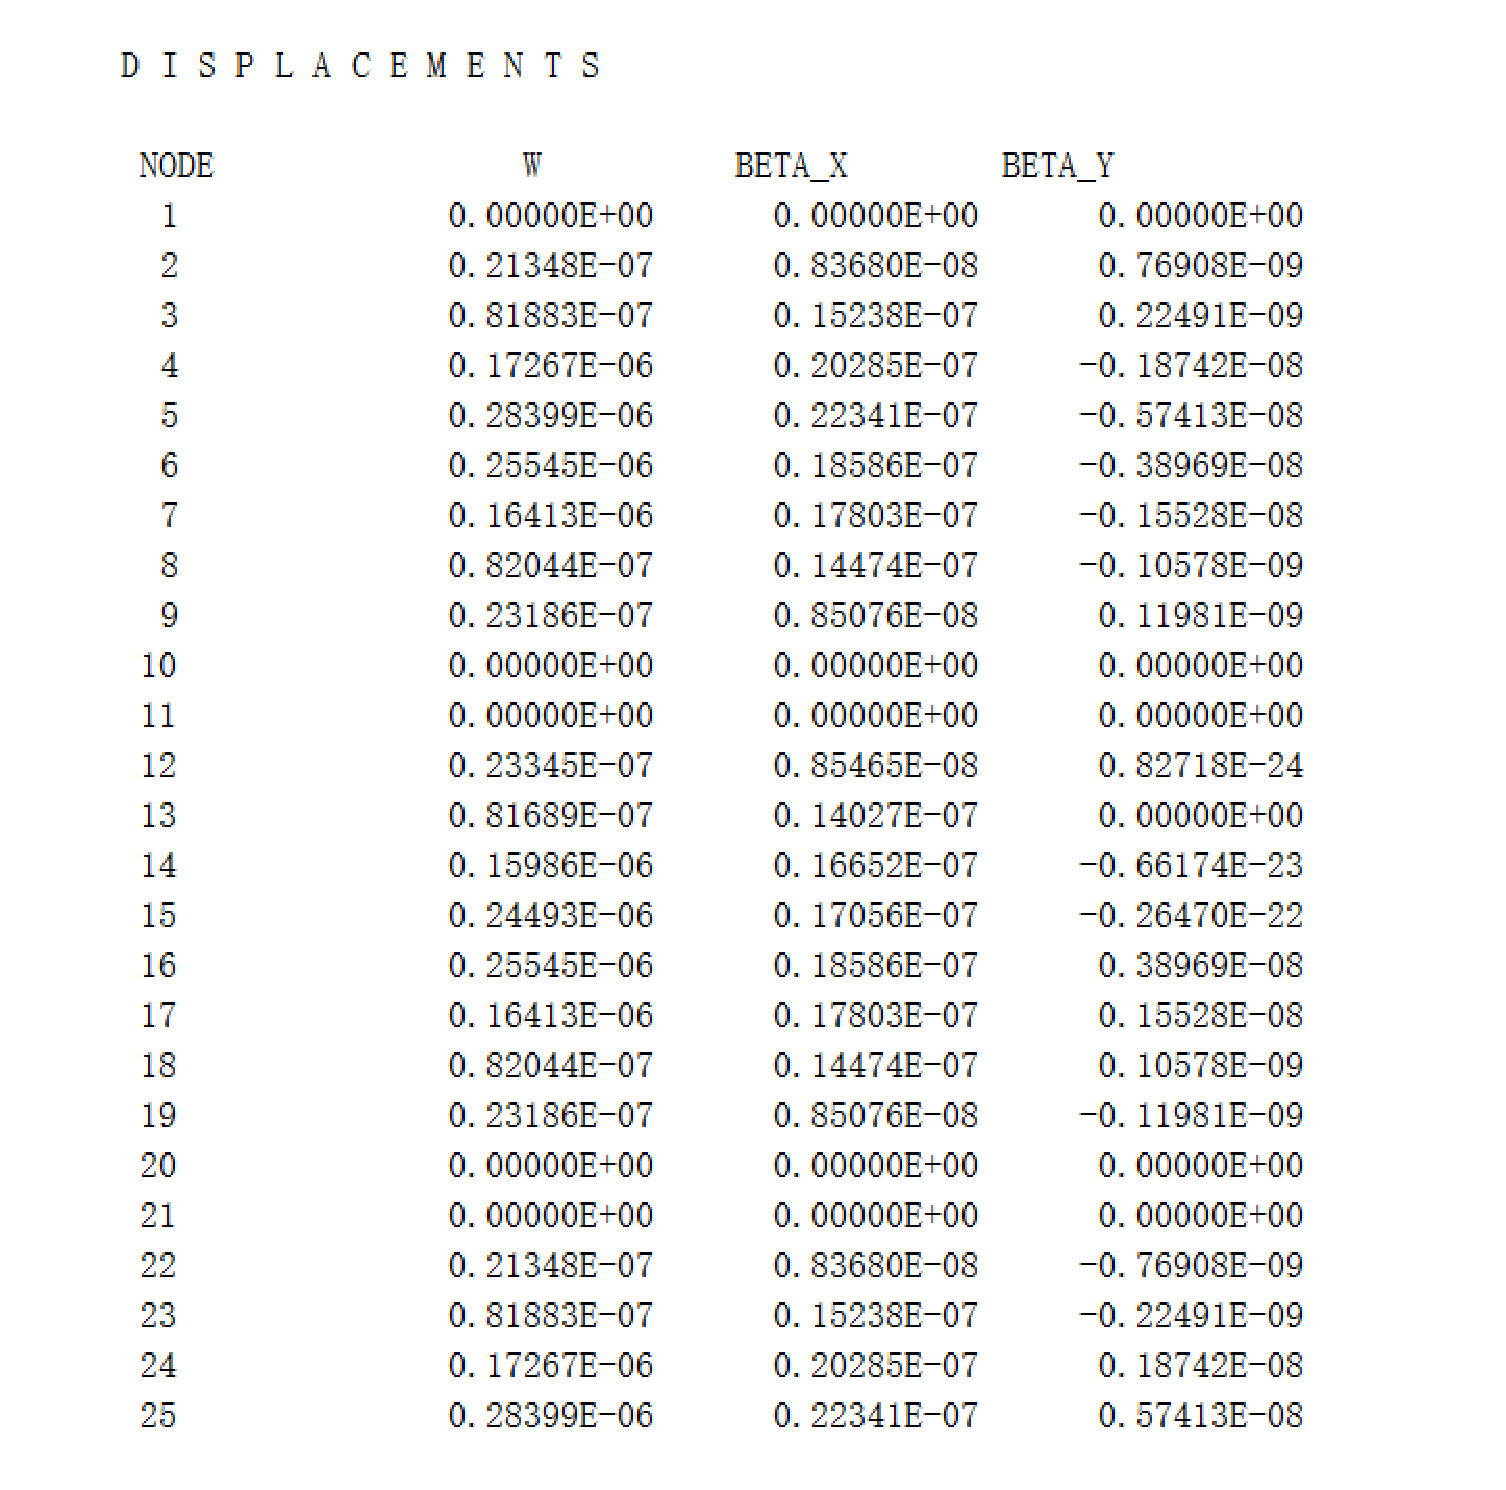
\includegraphics[width=7.23cm,height=7.15cm]{plate4Q_appl.pdf}
        \end{center}
    Since the elements are still few, it is nice to have the same scale. And the plate8Q is better.

\subsection{无限单元}

\subsection{超级单元}

\subsection{过渡单元}

此处的过渡单元为5节点,过渡4Q与9Q单元,使其衔接起来

PatchTest所使用的构型仍为4Q使用的Patchtest方案,即约束左下角两个自由度的位移,以及右下角Y自由度的位移,在顶部施加向下为20N/m的均布力。

其结果如下:
\begin{center}
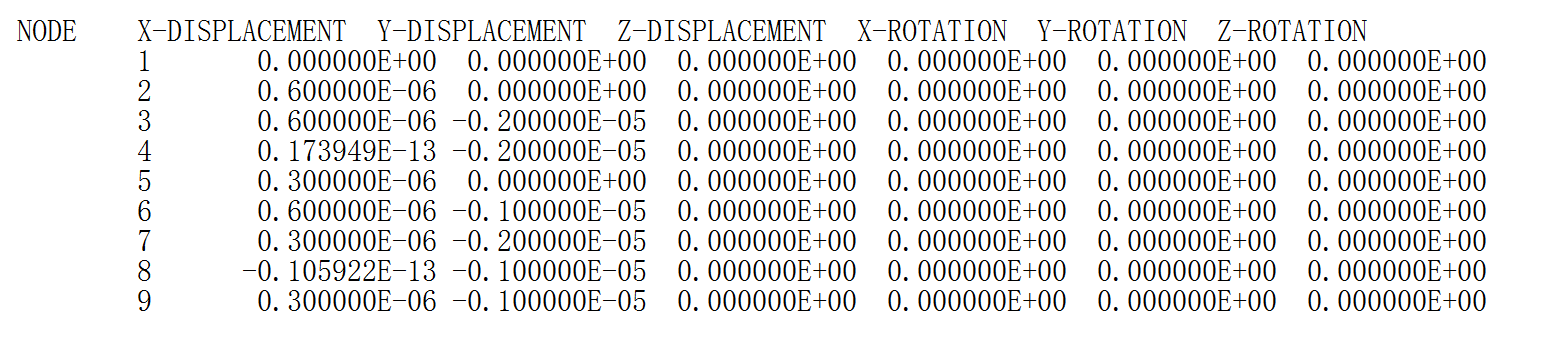
\includegraphics[width=\textwidth]{9Q02.png} % Include the image placeholder.png
\end{center}
\begin{center}
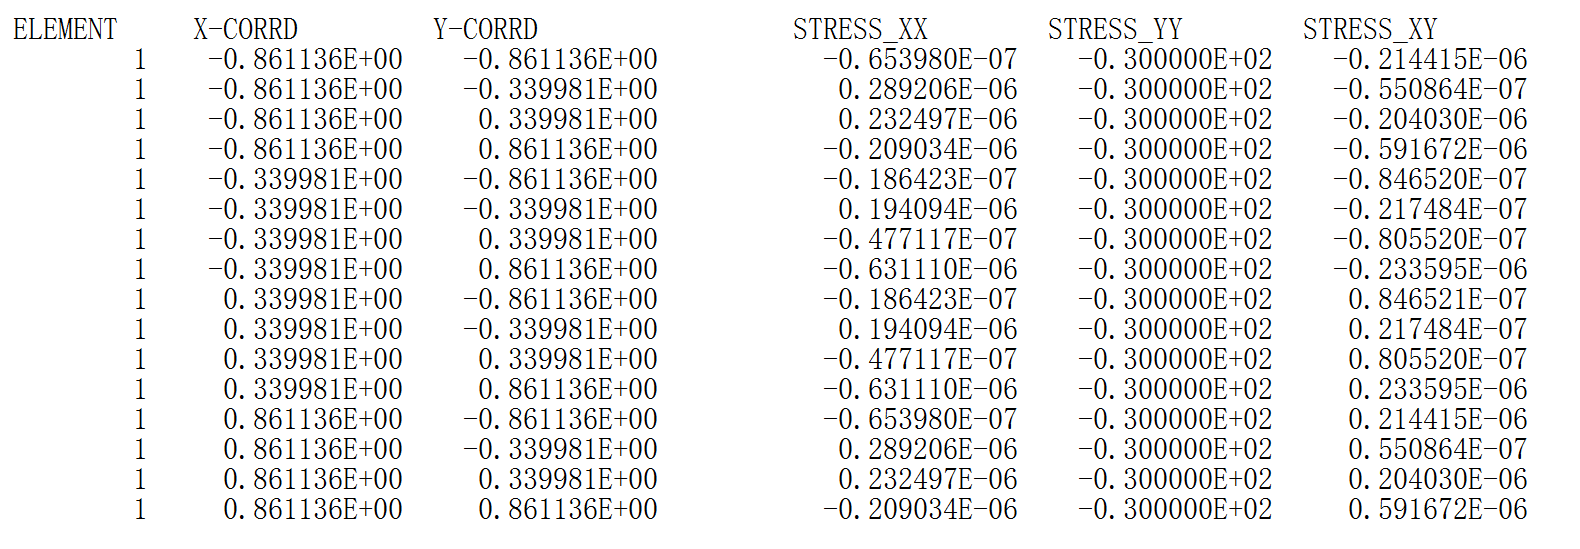
\includegraphics[width=\textwidth]{9Q03.png} % Include the image placeholder.png
\end{center}

使用连接算例如图:

%-------------------------这里是其他功能的描述-------------------------------------
%----------------------------------------------------------------------------------
\section{高级功能}
\subsection{弹塑性杆分析}





\subsubsection{基本原理}
\paragraph{}
弹塑性杆是一种最简单的材料非线性问题。在这个功能中,我使用切线刚度法来进行求解。我把杆的塑性问题简化成弹性段和塑形段,其中每段近似成线性函数,并使用相应的弹性模量和塑形模量来表示两端线段的斜率。切线刚度法的基本思想就是:假使载荷为$P_A$时,相应的位移为$u_A$,切线刚度为$K_A$,那么对于下一次载荷增量产生的位移是,
$$K_A\triangle u_{AB}=\triangle f_{AB}$$
$$u_B=u_A+\triangle u_{AB}$$
我们在使用切线刚度法进行计算时,都是从A点的应力状态出发,最后就得到载荷B情况下的各项参数,本方法的特点是,对于一次载荷分量,只需要求解一次即可。
示意图如下。
\begin{center}
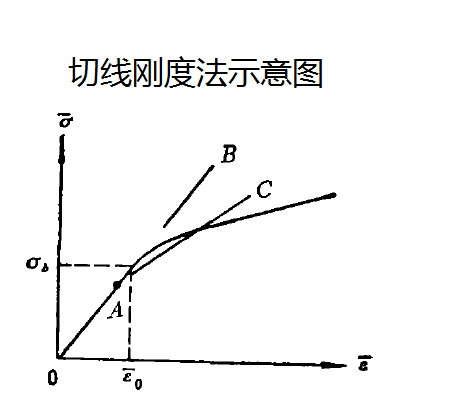
\includegraphics[width=0.6\textwidth]{plastic7.png}
\end{center}
该方法参考了1982年固体力学学报《弹塑性有限元一些解法的比较》,由中科院力学研究所吴永礼先生著。
\subsubsection{编程思路}
\paragraph{}
首先进行弹性试探步的计算,确定是否需要进行弹塑性分析。若进行弹塑性分析,则使用切线刚度法求解。首先把载荷分成很多细份,从零开始逐渐加载。使用切线刚度,算出每一步的位移增量和应力增量,计算每步加载后的位移和应力,同时判断是否有杆进入弹塑性,若有弹塑性变化,则下一次组装刚度阵时要更新。这种增量步的方法把一个非线性的问题线性化,实质上是微分的思路——把复杂的函数简单化,理论上,这种求解方式可以进行任何材料非线性问题的计算。在这个方法中,每一步更新需要前一步的历史位移和应力信息,这些都记录在临时文件里,每一步均更新。
整个程序的流程图如下。
\begin{center}
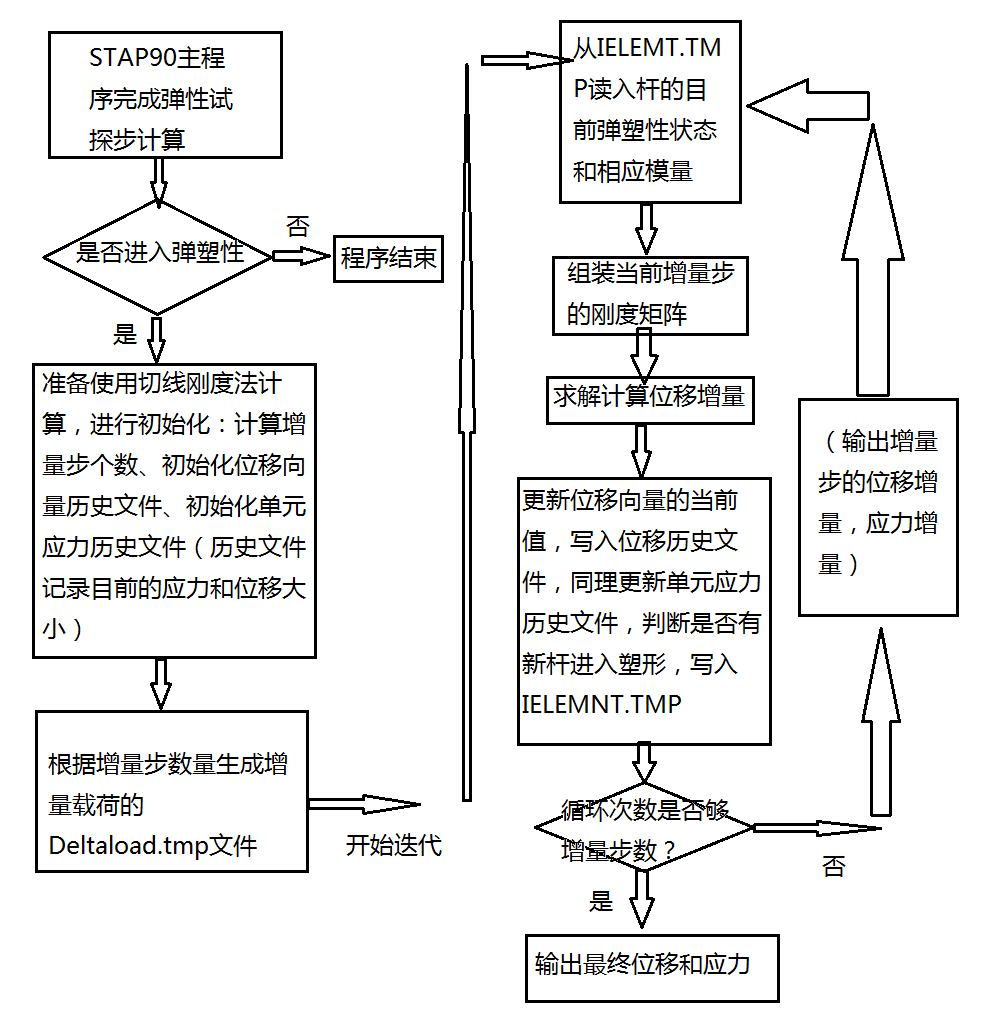
\includegraphics[width=0.9\textwidth]{plastic3.png}
\end{center}
\subsubsection{输入和输出结果}
\paragraph{}
在一根杆上加了100000的力,材料的截面性质如下,各输入和输出如下,结果符合理论值。
\begin{center}
\includegraphics[width=0.5\textwidth]{plastic2.png}
\end{center}
\begin{center}
\includegraphics[width=0.8\textwidth]{plastic1.png}
\end{center}
\begin{center}
\includegraphics[width=1.0\textwidth]{plastic4.png}
\end{center}
\begin{center}
\includegraphics[width=1.0\textwidth]{plastic5.png}
\end{center}
\begin{center}
\includegraphics[width=1.0\textwidth]{plastic6.png}
\end{center}
\subsection{模态分析}
\subsubsection{背景}
\paragraph{}
N自由度无阻尼线性系统作微幅振动,最后可得到振动微分方程组:$\boldsymbol{M\ddot x+Kx=0}$。分析一个弹性体的模态,实质是求解广义特征值问题$\boldsymbol{K-\lambda M=0}$,再由$\boldsymbol{\omega =\lambda}^{1/2}$得到系统的特征频率。对于多自由度系统,往往只有最小的数个特征值,即对应的几个频率最低的模态对结构具有关键作用。搜索最小数个特征值的算法常见的有LANCZOS迭代法,子空间迭代法等。本程序针对刚度阵、质量矩阵采用Skyline存储方式试图采用LANCZOS迭代法对广义特征值问题进行求解,另外针对稀疏矩阵的CSR存储方法,也提供了基于Intel MKL的feast算法库的调用。测试计算采用杆单元,但对大多数单元都加入了组装质量阵的模块,理论上可以进行模态分析。测试结果如Samples/Modal文件夹中所示。
\subsubsection{算法分析}
\paragraph{}
LANCZOS迭代法,其基本思路为利用里兹法求解特征值问题:
\begin{enumerate}
\item 选取与所有已求得的特征向量正交的初始迭代向量$\hat{x}_{1}$,并进行正则化:$x_{1}=\frac{\hat{x}_{1}}{\beta_{1}},\ \beta_{1}=(\hat{x}_{1}^{T}M\hat{x}_{1})^{1/2}$
\item 选取一移轴量$\mu$,生成Lanczos基向量:


$(K-\mu M)\widetilde{x}_{i}=Mx_{i-1},\ a_{i-1}=\widetilde{x}_{i}^{T}Mx_{i-1},\ \widetilde{x}_{i}'=\widetilde{x}_{i}-a_{i-1}x_{i-1}-\beta_{i-1}x_{i-2},$


$\hat{x}_{i}=\hat{x}_{i}'-\sum_{k=1}^{i-1}(\hat{x}_{i}'^{T}Mx_{k})x_{k}-\sum_{j=1}^{n_{c}}(\hat{x}_{i}'^{T}M\phi_{j})\phi_{j},\ \beta_{i}=(\hat{x}_{i}^{T}M\hat{x}_{i})^{1/2},\ x_{i}=\frac{\hat{x}_{i}}{\beta_{i}}$

\item 求解$Tz=\frac{1}{\lambda}z$,得到在本次迭代中收敛的特征值及对应的特征向量,如果收敛个数超过所需个数,则停止迭代,否则转1.\end{enumerate}


\subsection{动力学响应分析}

\end{document}
